\documentclass[12pt,listof=numbered,pagesize,bibliography=totocnumbered,oneside]{scrreprt} 
%Schriftgröße, zufälliges zeug, zufälliges Zeug, Literaturverzeichnis bekommt eine Nummer im Inhaltsverzeichnis
%scrreport weil anders als Article gibt es auch chapters, aber es ist nicht nötig herumzufuchsen um bei jedem chapter das Kapitel:XXX weg zu kriegen

%%%%%%%%%%%%%%%%%%%%% CITATIONS & LANGUAGE

\usepackage[british]{babel} %für die Worttrennung, das Datum, die Bibliographie usw...
\usepackage[utf8]{inputenc} %sonst gibts kein ß usw
\usepackage{csquotes} %sonst beschwert sich Biber

% BIBLIOGRAPHY AND CITATION STYLE
\usepackage[
maxcitenames=3,
backend=biber,
style=apa,
citestyle=authoryear
]{biblatex} %biblatex mit biber laden 
\ExecuteBibliographyOptions{
sorting=nyt, %Sortierung Autor, Titel, Jahr 
bibwarn=true, %Probleme mit den Daten, die Backend betreffen anzeigen 
isbn=false, %keine isbn anzeigen 
url=false, %keine url anzeigen 
doi=false
}
\addbibresource{Bib.bib} %Bibliographiedateien laden 

\DeclareLanguageMapping{british}{british-apa}

\DefineBibliographyStrings{british}{ %has to be same as Babel!
   andothers = {{et\,al\adddot}},             
} 
%%%%%%%%%%%%%%%%%%%% FORMAT

%% PAGE DIMENSIONS
\usepackage{geometry} % to change the page dimensions
\geometry{a4paper} % or letterpaper (US) or a5paper or....
\geometry{top=2.5cm, bottom=2.5cm, left=3cm, right=2.5cm} %wie in der Formatvorlage definiert

%% LANDSCAPE
\usepackage{lscape} %\begin{landscape} ... \end{lanscape}

%% FONT
\usepackage{helvet}
\renewcommand\familydefault{\sfdefault}
\usepackage[T1]{fontenc}

% SIZING OF SECTION HEADERS
\setkomafont{chapter}{\LARGE}
\setkomafont{section}{\Large}
\setkomafont{subsection}{\large}
\setkomafont{subsubsection}{\normalsize}
\setkomafont{paragraph}{\normalsize}
\setkomafont{subparagraph}{\normalsize}

%SIZING OF CAPTIONS
\usepackage[font=small]{caption}

% FONT SIZE
\makeatletter 
\renewcommand\LARGE{\@setfontsize\LARGE{16pt}{19}}
\renewcommand\Large{\@setfontsize\Large{14pt}{17}}
\renewcommand\large{\@setfontsize\large{12pt}{15}}
\renewcommand\small{\@setfontsize\small{10pt}{10}}%Abbildungs-,Tabellenbeschriftung und Fußnote
\makeatother

%% SPACE AROUND SECTION HEADERS
\RedeclareSectionCommand[
  beforeskip=.7\baselineskip,afterskip=.3\baselineskip]{chapter}
\RedeclareSectionCommand[
  beforeskip=.7\baselineskip,afterskip=.3\baselineskip]{section}
\RedeclareSectionCommand[
  beforeskip=1\baselineskip,afterskip=.3\baselineskip]{subsection}

%% GENERAL SPACING
\usepackage[onehalfspacing]{setspace}
% \usepackage[doublespacing]{setspace}

%% HEADER AND FOOTER
\usepackage{scrlayer-scrpage}
%\pagestyle{myheadings}
%\plainheadsepline=true
\lefoot*{A New Drop Test Rig for Kiirunavaara Mine}
\refoot*{Page \pagemark}


%\pagestyle{fancy}
%\fancyhf{}
%\lfoot{Interim Report}
%\lfoot{A New Drop Test Rig for Kiirunavaara Mine}
%\rfoot{Page \thepage}

% Redefine the plain page style
%\fancypagestyle{plain}{%
%  \fancyhf{}%
%\lfoot{A New Drop Test Rig for Kiirunavaara Mine}
%\rfoot{Page \thepage}
%}

%% FRONTPAGE

% DATE
\usepackage[en-GB]{datetime2} 

% TABLE (GRAY LINES)
\usepackage[table]{xcolor} %to make nice gray lines on the title page

%%%%%%%%%%%%%%%%%% STUFF I NEED

\usepackage{graphicx} % support the \includegraphics command and options

\usepackage{subcaption} % make it possible to include more than one captioned figure/table in a single float

% ° 
\usepackage{textcomp} 

% SECOND TOC
\usepackage{titletoc} 
\dottedcontents{section}[4.6em]{}{3pc}{-1pc}
\dottedcontents{subsection}[7.7em]{}{3pc}{-1pc}
\makeatletter
\renewcommand\@dotsep{500}   % default value 4.5
\makeatother

% INPUT PDFs
\usepackage{pdfpages}

% NICER ARRAYS
\usepackage{array} 

% COMMENT SECTIONS WITH \begin{comment} ...  \end{comment}
\usepackage{comment} 

%%%%%%%%%%%%%%%%% TABLES

\usepackage{multirow}

\renewcommand{\arraystretch}{1.2}

\usepackage{booktabs,ragged2e}

\newcolumntype{P}[1]{>{\RaggedRight\arraybackslash}p{#1}}

%%%%%%%%%%%%%%%% MATH


\usepackage{amsmath} %math stuff
\usepackage{mathtools} %nice looking math stuff
%\newcommand*\rfrac[2]{{}^{#1}\!/_{#2}} %shorter fractual, \rfrac{top}{bottom}
\newcommand{\rfrac}[2]{\frac{\text{#1}}{\text{#2}}} %shorter fractual, \rfrac{top}{bottom}

%%%%%%%%%%%%% TIKZ

\usepackage{tikz} % NOT drawing
\usetikzlibrary{
    arrows.meta,
    calc,
    datavisualization,
    patterns,
    shapes.arrows
    }
    
\usepackage{tikz-3dplot}
%%%%%%%%%%%%%% REFERENCING

\usepackage{hyperref}


%%%%%%%%%%%%% working title
\author{Karin Ungerer}
\date{\today}
\title{Interim Report}


\begin{document}

\startcontents[main]


\begin{titlepage}

\raggedleft{
\includegraphics[scale=0.15]{pics/MUL.jpg}}
\textcolor{gray}{\rule{\textwidth}{0.2pt}}
%\textcolor‎{‎gray}{\rule{\textwidth}{0.2pt}}

\vspace{2pt}

\raggedright{\large {Master Thesis}} 

\vspace{2pt}

\textcolor{gray}{\rule{\textwidth}{0.2pt}}

\vspace{1cm}

\centering

\huge \textbf {A New Drop Test Rig for Kiirunavaara Mine}

\vspace{1cm}

\textcolor{gray}{\rule{\textwidth}{0.2pt}}

\vspace{\fill}

\large \textbf {\LARGE{Karin Ungerer}}
\\

\vspace{\fill}

\small
\raggedleft
\singlespacing
%\bgroup
\arrayrulecolor{gray}
\begin{tabular}{ r | r }
\today  & 
\includegraphics[width=0.2\textwidth]{pics/Logo.png}
\\ \hline   
Department Mineral Resources Engineering\\
Lehrstuhl für Bergbaukunde, Bergtechnik und Bergwirtschaft \\ 
Montanuniversität Leoben\\
A-8700 LEOBEN, Franz Josef Straße 18 \\
Tel.Nr.: +43 3842-402-2001\\
Fax: +43 3842-402-2002\\
bergbau@unileoben.ac.at &  
\end{tabular}
%\egroup

\end{titlepage}


\pagenumbering{Roman}
\setcounter{page}{2}

\normalsize

\chapter*{Declaration of Authorship}
\addcontentsline{toc}{chapter}{Declaration of Authorship}

„I declare in lieu of oath that this thesis is entirely my own work except where
otherwise indicated. The presence of quoted or paraphrased material has been clearly
signaled and all sources have been referred. The thesis has not been submitted for a degree
at any other institution and has not been published yet.”

\chapter*{Preface}
 \addcontentsline{toc}{chapter}{Preface}
%
%Eloquent expression of my gratitude towards everyone involved in this thesis.

How often do you get the chance to say, that for one short moment in time, you were the best at something? 
\textcite[93]{Heal10} states, that the drop test rig built by WASM is the most sophisticated and best instrumented rig, in the world today. As it is his Alma Mater, he added a modest "perhaps". 
Reading those lines motivated me beyond believe, I knew we had the potential to be better and I knew I wanted to be better. This is why I have to thank Daniel Heal first and foremost.

Secondly I have to thank Biruk Woldhemedin who had to endure the bulk of my misguided enthusiasm and crazy ideas and who kept his humor and his patience even as I cleaned his whiteboard or made fun of his palm tree and helped me navigate the treacherous rapids of Swedish culture. Keep on being awesome.

I want to thank my supervisors at Montanuniversity Leoben, Horst Wagner and Tobias Ladinig for supporting me and not giving up on me, even when I acted too laissez-faire for their taste or sent them too many too long emails.

Matthias Wimmer, I must thank you for making this possible and supporting me with everything. 

I want to thank SODA, the board game club of Kiruna, and all of its members for helping me keep my sanity through the long dark polar night and the long bright polar day. My role-play friends: Adam, Jule, Robert, Tony, William and Flimbimsy. I hope you enjoyed roaming the galaxy and victorian London as much as I did.
Especially Ingrid, thanks for your support with my real and fictional relationship troubles. I felt more at home in your apartment than anywhere I lived in the past few years. 

I want to thank my family and friends for supporting me. My sister who found time for me next to her two studies, two cats and everything else. My friends in Leoben who kept in contact even though I was so far away.
Erik, thank you for enduring long hours of talking about our feelings, great recommendations in music and movies and your patience.
Gü, you helped me a lot with your spreadsheets, your interesting ideas and your patience with my silliness. 

With this, all that is left for me to say is: good luck to the next person who gets to work with this rig. I hope this thesis, my notes, my code and the decisions I made help you more than they hinder you and I look forward to reading what you manage to do with this impressive machine. Good luck.

\chapter*{Abstract}
\addcontentsline{toc}{chapter}{Abstract}

%This thesis is concerned with the testing of surface support elements under dynamic loading conditions. 
%Firstly there's some literature and definitions and some previous tests by other people are described.
%Secondly the test rig and test method and its limits are described.
%Thirdly results of the tests are presented and discussed.
%Lastly the best possible surface support structure is discussed in detail and recommended further steps are given.

In order to optimize the energy absorption capabilities of the surface support system, Kiirunavaara mine, owned by LKAB, has constructed a drop test rig. It has a drop height of up to 4 m and a maximum drop weight of 1000 kg. Load cells, laser distance measurements, high speed camera footage and multiple accelerometers ensured comprehensive data collection.

It is capable of testing round discrete concrete samples with a diameter of 0,8 m (after \textcite{c1550}) and square concrete samples with an edge length of 1,5 m. The square samples are cast on top of large concrete slabs that serve to simulate the adhesion between shotcrete and rock. It is possible to test different types of mesh with varying boundary stiffness and rate of pretension as well as different types of lacing and straps. Concrete, mesh and lacing can be freely combined, therefore it is possible to test various surface support concepts. 

Several tests were run with this test rig. The tests were focused on optimising the rig and all changes that were made are discussed in detail. From the results of the first tests is was possible to devise equations that allow to estimate the energy absorption capabilities of shotcrete at different thicknesses.

Later campaigns will test the support system currently in use at Kiirunavaara Mine as well as some modifications of it.
%The results of these test are presented and discussed in detail.

Lastly future modification that could be done to make the rig more comprehensive are discussed, for example being able to conduct dynamic tests on bolts, quasi-static tests on surface support or dynamic tests on complete support systems. %It also provides some ideas for future test matrices.
Some ideas for future test matrices are given.

%%%%%%%% TO DO Talk about results

%The goal of the first test series run with the rig was to find potential enhancements and increase the credibility of the results of further tests. Round samples were used for this test.

%When the rig had been modified sufficiently, tests on large square samples were conducted. The tested materials included: fibre reinforced concrete, welded mesh, chain-link mesh, lacing, straps ("Fjällband"). The boundary conditions of the tested meshes were considered at length.



%A small series of tests was run on round samples with a diameter of 800 mm. This report discusses the findings of those tests and the potential of the rig.

%The results of the test show quite clearly that the test procedure would benefit from functioning way of measuring displacement and that the energy absorption capabilites rise with the thickness of the concrete panel, as expected. 

%The currently used method of measuring displacement by a laser sensor suffered some complications. The way displacement is measured will have to be reconsidered. The analysis of the test data was greatly affected by the lack of displacement data, therefor not many conclusions could be drawn. It mainly became apparent that the energy absorption capabilities of the test panels rose with the thickness of the panels.

%Using the findings of this report the testrig will be optimized so that the tests on the large samples will have good results.

%\chapter*{Zusammenfassung}
% \addcontentsline{toc}{chapter}{Zusammenfassung}

\newpage

\printcontents[main]{}{0}{}
\addcontentsline{to_c}{chapter}{Table of Contents}
\cleardoubleoddpage

\pagenumbering{arabic}
\setcounter{page}{1}

\chapter{Introduction}

%Allgemeines über Gebirgsmechanik
\begin{quote} 
\textit{``Rock fails because the stresses overcome the rockmass strength.''} \\
\autocite[2.13]{canada96}
\end{quote} 
This the basic principle behind rock mechanics. It's not possible to change the inherent strength of the rock, only to enhance it through rock support. \autocite{Hoek80} %The stresses are caused by forces that are applied to the rock mass. 

%%%%%%%%%%%%%%%% difference between static and dynamic loading
%TO DO put something here!

%Usually rock support has to withstand static load. The difference between static and dynamic load is best described by \textcite{Timo56} who states that ``Statics deals with the conditions of bodies acted upon by forces'' whereas dynamics is defined as ``the relationship between the kind of motion of a particle and the forces producing it''. From this definition it becomes obvious that dynamic load is connected to movement, whereas static load is motionless. Of course, there is no pure static load in mining, rock creeps and deforms, therefore it´s preferable to refer to this state as quasi-static.


There are two types of stress inside the rock mass: quasi - static stress and dynamic stress.
Dynamic stresses can be caused by seismic events. An easy way to distinguish between static and dynamic stresses is the strain rate  (\( \dot{\varepsilon} \)).  \( \dot{\varepsilon} \) means the change in length per second. After \textcite{strain04}: $\dot{\varepsilon} = \int \frac{l(t)}{l_0} dt  $. With $l(t)$ as the size at a given time and $l_0$ as the size at $t=0$. \textcite[3]{ali2002} stated that static load causes \( \dot{\varepsilon} \) of approximately $ 10^{-5}~\text{s}^{-1} $. 
Compared to that, dynamic loading, specifically seismic events, can cause \(\dot{\varepsilon} = 5 * 10^{-3}~\text{s}^{-1}~ \dot{\varepsilon}\) while blasting can reach up to can cause \(\dot{\varepsilon} = 10^{3}~\text{s}^{-1}~\). The strain rate during seismic events is much higher than the strain rate under static loading conditions. 
\textcite[6]{reinhardt82} stated that a seismic event may cause loading rates of up to 100 \(\frac{\text{N}}{\text{mm}^\text{2}}*\text{ms}\).  %Seismic events can be characterized by a several parameters including: amplitude of the the seismic wave, released energy and distance from the observer. These parameters influence the tensions inside of the rock and the demands on the rock support. 
%Type of seismic event
\section{Different Types of Seismic Events}
\textcite[3]{player04} defined a seismic event as: "A release of built up strain energy." %from the formation of excavations that does not result in a fall of ground or yielding of ground control scheme
The released energy travels through the rock in the form of a wave. It possesses an amplitude and a frequency.
 According to \textcite{durrheim06} seismic events can be grouped in 3 categories according to their relation to mining activity:
 
 \begin{itemize}
     \item Natural
     \item Mining triggered
     \item Mining induced
 \end{itemize}
 
A natural earthquake is not caused or influenced by human activity.%, especially mining, in any way. 

A mining triggered earthquake only happens along a pre-existing fault. Mining activity triggers these events but is not the driving force.
%contributes only a small fraction of the observed energy. 
These events can happen at considerable distance to mining operations.

Mining induced events are directly caused by mining. Most of the observed energy stems directly from mining activities or mining related stresses. They often happen along pre-existing faults or create new ruptures. 

The resulting tensions in the rock mass depend
%The demands such an event puts on the rock mass are dependant 
The resulting tensions in the rock mass depend on several factors: the magnitude of the triggering seismic event, the rate at which it releases its energy and the distance from the hypocentre of the event. %as well as the properties of the rock in between hypocenter and excavation as well as directly around the excavation.
If the demands of the seismic event exceed the capabilities of the rock support, it will fail. A failure of the rock support and the associated consequences, such as ejected rock, are summarized under the term rockburst.
It is crucial to differentiate between the seismic event and the observed damage mechanism. \autocite{Kaiser12} \autocite[9]{Heal10}

%Damage mechanism
\section{Damage Mechanism}

%There are several different modes failure under of dynamic loading, they are in general combined under the term ``rockburst''. 
%\textcite{Hoek80} defines rockbursts as: ``Rockbursts are explosive rock failures which can occur when strong brittle rock is subjected to high stress.'' which is a very general definition focusing on rock mechanics. Most definitions put the different failure modes more into the foreground. For example 
%\Textcite[271]{Brady99} defines rockbursts: "A rockburst is the sudden displacement of rock, under seismic impulse, in the boundary of an excavation, causing substantial damage to it." 
%which only describes a very specific type of damage mechanism.
%\textcite{Brauner94} defines rockbursts as: ``Rockbursts are violent failures in the ground, breaking rock and expelling it into excavations.'' 
%On the other hand \textcite[582]{Obert67} provides following definition ``A rockburst is defined as any violent expulsion of rock from its surroundings, the phenomenon resulting from static stress exceeding the static strength of the rock'' This definition introduces another important factor: static stress. %With this definition in mind it becomes obvious that Static stress is necessary to cause dynamic loading. Though
\textcite[582]{Obert67} defined rockbursts as: 
 "any violent expulsion of rock from its surroundings, the phenomenon resulting from static stress exceeding the static strength of the rock''

High static stress and sufficiently brittle rock are needed to create rock bursts. \autocite[6]{Brauner94} \autocite[2.10]{canada96} Which is why Kiirunavaara Mine had only minor problems with rockbursts until the rock mass quality significantly increased at a depth of around 900 m. The reason for this increase is unclear. \autocite[4]{dahner12} %became significantly more brittle 
 Static stress in general increases with depth, that is why vulnerability to rockbursts is usually thought to increase with depth. \autocite[8]{Brauner94}

There are records of very deep mines which are seismically inactive as well as of rockbursts in open pit mines or at shallow depths. %Especially in Australia because of the high vertical stresses present in the ground. 
\autocite[584]{Obert67} Other factors than depth must also influence how burst prone ground is.
%Other factors also influence how burst prone the rock mass is. 
  %the magnitude of the triggering seismic event, the rate at which it releases its energy and the distance from the hypocenter of the event to the excavation. 
Rock properties like rock type, rock strength, joint fabric and rock brittleness influence the behavior of the rock. The stress distribution is influenced by the existence of geological structures, mining induced static stresses, the span of the excavation, the extraction ratio, the production rate, the  mine stiffness, the layout of the mine and if backfill is used, the properties of the backfill material.  \autocite[2.10]{canada96} \autocite[219]{Kaiser12} \autocite[8]{Brauner94} 


The level of the dynamic stress in the rock mass also depend on the seismic event itself.
%The amount of dynamic load that the rock mass has to take is also an important factor. 
%The amount of dynamic stresses inside the rock mass is also an important factor. 
As previously discussed the stresses caused by a seismic event can be roughly estimated from the released energy, the rate at which this energy is released and the distance from hypocenter. To describe the amount of energy released by a seismic event the Richter scale can be used.
But not all rockbursts are equal, they can take different forms depending on various factors.
%\textcite[8]{Brauner94} writes: 
%\begin{quote} 
%\textit{''Even though other factors remain equal, both frequency and severity [of rockbursts] increases with depth.  This, however is overshadowed by influences of the local mining geometry, mainly the vicinity of other excavations.''}
%\end{quote} 

%In general rockbursts are cause by seismic events, either of natural or artificial origin, built up of stress in the affected area or other mechanisms. \autocite[24]{Brauner94} %They can happen seemingly at random in the case of bulking.\autocite[2.4]{canada96} 

%failure modes

%``Rockburst'' is also an umbrella term for a range of different failure modes. 
% The term "rockbursts" is applied to a range of different failure modes.
\textcite{Ortlepp97Fracture} defined the following failure mechanisms:

\begin{itemize}
\item strain burst
\item buckling
\item face crush/pillar burst
\item shear rupture
\item fault-slip burst
\end{itemize}

Strain bursting is a result of low Richter Magnitudes, between -0,2 and 0 and takes the form of superficial spalling with violent ejection of fragments. 
Buckling is a result of Richter magnitudes between 0 and 1,5. Large slabs or rock are expulsed into the excavation.
Face crush / pillar burst is a result of Richter Magnitudes between 1 and 2,5. As the name implies rock is violently expulsed from the stope face or the pillar sides.
Shear rupture is a result of 2 to 3,5 on the Richter Scale. Shear fractures violently propagate through the intact rock mass. 
Fault-slip describes violent movement along an existing fault. It is a result of 2,5 to 5 magnitude on the Richter Scale.

Under the right conditions, rockbursts will inevitably happen. \autocite[4]{Heal10} That is why it is important to learn how to reduce their frequency and severity.


\section{Reducing the Frequency and Severity of Rockbursts}
%what to do against rockbursts?
Essential in reducing the frequency and severity of rockbursts is reducing the stresses in the rock mass. There is a plethora of possible measures that can be taken in advance, for example: changing or modifying mining sequence, mining geometry, mining method, excavation shape, location of drifts and ore passes, stope size and using backfill or changing the properties of the backfill material. \autocite[219]{Kaiser12} As the vulnerability to rockbursts increases with excavation span, 4-way intersections should be avoided where possible. \autocite[323]{Heal10}
If a small area is dangerously overstressed, destress drill and blasting can be used to actively reduce the likelihood of a rockburst. \autocite[219]{Kaiser12}
Human safety can be increased through usage of remotely operated equipment. \autocite[3]{Heal10}
But rockbursts are impossible to predict reliably. \autocite[4]{Heal10} \autocite[10]{durrheim06} Measures such as destress blasting bring immediate release of tensions. But make the ground more prone to rocksbursts in the future by weakening the rock mass and increasing the amount of loose rock that can be mobilized during a rockburst. \autocite[61]{Brauner94} For certain applications destress blasting is incredibly useful but it is currently not used in Kiirunavaara mine.

\chapter{Rock Support}
%Rock support
The last line of defense against rockbursts is rock support. It is often also the most effective. \autocite[323]{Heal10}

%The maxim of surface support design in the Kiirunavaara Mine so far was very heavily based on the first concept with ever increasing thicknesses of shotcrete being applied as previous support concepts fail or after cleaning up rockfalls. This game can not be played indefinitely though. \textcite[2.17]{canada96} states that: \begin{quote}\textit{"As the rockburst severity increases, the support will not be able to prevent initiation of the damage mechanism. An appropriate support system must however be able to survive the displacements associated with the rockburst and remain functional after the rockburst to hold and retain broken rock."}\end{quote} It seems probable that the Kiirunavaara Mine is at a crossroads. Ever increasing static load is requiring stronger and stronger support in order to keep the rock mass from unraveling, while in some places catastrophic failures can be observed. It may worthwhile to invest heavier in yielding rock support. At this point in time it might be feasible to consider using reinforced shotcrete instead of mesh being attached over shotcrete or maybe even to progress as far as isolated shotcrete panels, in order to allow large initial deformations before the shotcrete panels are "activated".

%As soon as shotcrete tears, its support function is heavily impaired at this point the load must be taken by the welded mesh almost single handedly. This poses the question if the heavy use of shotcrete at Kiirunavaara is really cost effective. As explained in \autoref{sec:rockbursts} the main requirements posed by the currently observed failure modes are: abilty to survive heavy displacement as well as strong reinforcement of the rock mass. Which is difficult to archieve at the same time.
%(FIND THE PICTURES!) there are some rockfalls, where it is obvious that just the shotcrete and a thin layer of rock has been affected, with minor to moderate bulking being the failure mode. It is probable that a more flexible support system might have been able to absorb the excess energy through deformation. 

Rock supports main functions after \textcite{canada96} are maintaining the integrity of surrounding excavation, retaining fractured rock and preventing excessive excavation deformation.

\textcite{canada96} defined two kinds of support elements:% which full the 3 main functions:
\begin{itemize}
\item reinforcement support
\item surface support
\end{itemize}

\begin{comment}
\begin{table}
    \centering
    \begin{tabular}{l l p{5cm}}
        \toprule
        Displacement  & Energy Demand  & Recommended Bolt\\
         \(mm\)  &  \(\rfrac{kJ}{m^2}\)  & \\
         \midrule
        < 50 & < 5 & Expansion shell rock bolt, Resin/cement steel rebar\\
        50 - 100 & 5 - 15 & Split Set, Swellex, Roofex, Yield-Lok\\
        100 - 200 & 15 - 25 & Swellex, D-Bolt, Conebolt, Roofex, Yield-Lok\\
        200 - 300 & 25 - 35 & Roofex, Conebolt, Garford \\
        > 300 & > 35 & Conebolt, Garford\\
         \bottomrule
    \end{tabular}
    \caption{bolt recommendations after \textcite[580]{Masoudi18}}
    \label{tab:bolt}
\end{table}


\begin{figure}
    \centering
    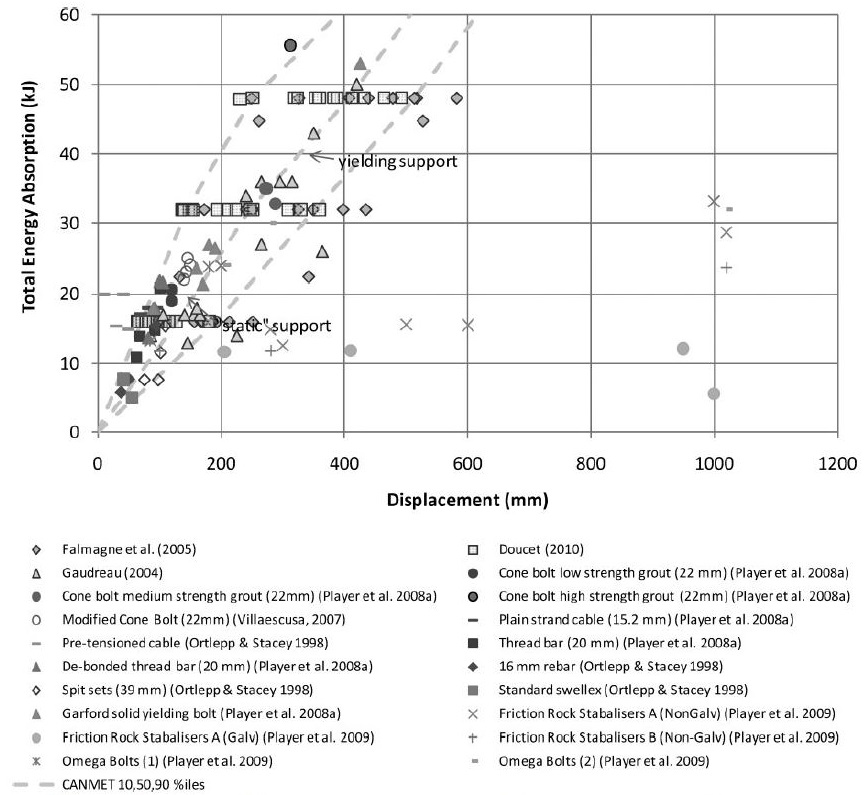
\includegraphics[width=0.9 \linewidth]{pics/potvin10_bolts.JPG}
    \caption{Compilation of the results various dynamic tests of bolts by \textcite{Potvin10}}
    \label{fig:potbol}
\end{figure}

\begin{figure}
    \centering
    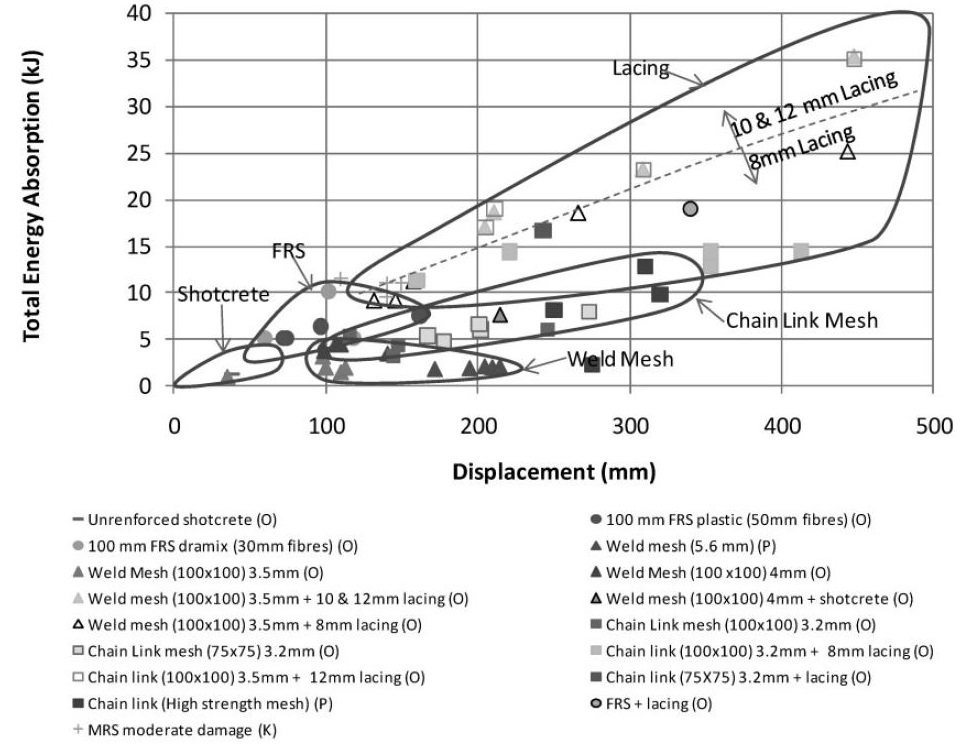
\includegraphics[width=0.9 \linewidth]{pics/potvin10_surface.JPG}
    \caption{compilation of the results various dynamic tests of surface support elements by \textcite{Potvin10}}
    \label{fig:potsur}
\end{figure}

\end{comment}
\section{Reinforcement Support}

%reinforcement support
\Textcite[312]{Brady99} defined reinforcement support as: "Means of conserving or improving the overall rock mass properties from within the rock mass".
%Reinforcement support elements have two functions: to increase the strength of the rock mass through reinforcement and to hold surface support elements in place. \autocite[2.16]{canada96} 
There are two design paradigms behind reinforcement support, depending on the rock conditions. One way is to contain deformations through anchoring large loose blocks to stable rock using widely spaced long bolts, which have to be able to survive large displacements. These long bolts directly secure large wedges and rocks to intact rock and high a high capacity to withstand deformations.
The other way is using tightly spaced short bolts with little displacement capabilities that deform with the rock. These short bolts confine highly fragmented rock mass around themselves and compact it into a "hard shell" around the excavation. \autocite[15]{guler01} These bolts do not deform themselves. They move with the rock that surrounds it.
Following the second paradigm it may be economical to install non-yielding bolts in burstprone ground. \autocite[6.23]{canada96}
%One kind of bolt may be used to satisfy both conditions but

In burst prone mines it often is more sensible to %have highly specialized bolts for try
have bolts for both of these tasks instead of just focusing on one. Especially in vulnerable areas such as intersections. Under quasi static loading conditions strength and cost are the deciding factors when designing a support system whereas burst prone ground requires high energy absorption capabilities and high displacement rates. %Nevertheless, it may be economical to install non-yielding bolts in burstprone ground. After a dynamic loading event, these bolts will have to be checked and possibly replaced. \autocite[6.23]{canada96} 
There are several kinds of bolts with varying suitability for use in burstprone mines. %, usually depending on their displacement and energy absorption capabilities. 
%Cone bolts, Swellex, Split Set bolts and debonded Cable bolts offer high displacement rates while at the same time having high peak load capacities. \autocite[4.14]{canada96} 
%In \autoref{tab:bolt} some bolt types and their dynamic capabilities are given. In \autoref{fig:potbol} the results of several dynamic tests of rock bolts are displayed. 

\begin{figure}
    \centering

\subcaptionbox{Square spacing of bolts}{\begin{tikzpicture}
%SQUARE spacing
\path (0,0) -| (7,7);

\foreach \x in {1,2,...,6}{
\foreach \y in {1,2,...,6}{
\draw[fill = black] 
(0+\y,0+\x) circle [radius=0.1]
;}}

\end{tikzpicture}}
\subcaptionbox{Diamond spacing of bolts}{\begin{tikzpicture}
%diamond spacing
\path (0,0) -| (7,7);

\foreach \x in {1,2,...,6}{
\foreach \y in {2,4,6}{
\draw[fill = black] 
(0+\x,0+\y) circle [radius=0.1]
;}}

\foreach \x in {1,2,...,6}{
\foreach \y in {1,3,5}{
\draw[fill = black] 
(0.5+\x,\y) circle [radius=0.1]
;}}

\end{tikzpicture}}

    \caption{Different ways of placing bolts}
    \label{fig:spacebolt}
\end{figure}

Bolt spacing is also an important factor. Diamond spacing is superior at load distribution but square spacing allows for easier installation of mesh with less overlap. \autocite[4.14]{canada96} See \autoref{fig:spacebolt}.
Tight bolt spacing prevents rock ejection. \autocite[217]{Heal10}
%Another important factor is bolt plate size, thickness and surface contact as well interaction between plate and washer. 
The bolt plate is the contact point between reinforcement support and surface support and therefore very important.

\section{Surface Support}
%surface support
One of the functions of surface support, in a dynamic context, is to transfer energy to the reinforcement support. \autocite[210]{Heal10} %In dynamic and purely static use cases surface support has retain broken rock and keep it from falling into the excavation. \autocite[2.16]{canada96} 
Another function is to retain broken rock and to keep it from falling into the excavation. \autocite[2.16]{canada96} Broken rock has be retained both under static stress and during dynamic loading events.

%Surface support elements basic function is to retain broken rock. \autocite[2.16]{canada96} Its secondary function, in a dynamic context, is to transfer energy to the reinforcement support. \autocite[210]{Heal10} 

%Unless lacing, straps or high tensile mesh is used as surface support, the surface support will likely fail before the bolts and at low energy levels. \autocite[240]{Potvin10}
%In \autoref{fig:potsur} the results of several dynamic tests of surface support elements are displayed.

Surface support elements are very diverse. 
Reinforced shotcrete (either with fibres or mesh), welded mesh, chain-link mesh, textile mesh, straps and lacing are typical surface support elements. %Deploying lacing is one way to control large displacements. 
Shotcrete is the stiffest surface support element and most commonly used. \autocite[4.38]{canada96} Shotcrete covers the entire surface of the excavation face and stabilises it. The most common form of shotcrete in use in mining is fibre reinforced shotcrete, FRS. Shotcrete performs well under compressive force, it cracks quickly under tension. It is activated by very small deformations before the rock mass begins to yield. \autocite[578]{sme11} Small surface deformations are therefore contained and spalling is reduced/prevented. \autocite[585]{sme11}
 \autocite[3]{Villa14}. If the stiff support of shotcrete is not necessary a similar effect can be achieved with thin spray on liners TSL. \autocite[22]{guler01} TSL have a thickness of about 5 mm and the technology is not yet fully developed or deployed a large scale. \autocite[591]{sme11}
The are more deformable than shotcrete and can distribute the load on a larger area. \autocite[58]{Guner18}   TSL can be applied directly on the rockmass or on a stabilising a layer of shotcrete. Spraying directly on the rock face is preferable because TSL can infiltrate cracks and gaps and stabilize the rock mass this way. \autocite[113]{archibald92} Some types of TSL hinder the flow of gases. In one trial conducted by \textcite[13]{archibald97} TSL proved 99,8\% effective at stopping the flow of radon. This very low penetrability makes TSL vulnerable to damage by blast gases. \autocite[19]{archibald97}
The reaction forces in TSL under compressive stress are negligible compared to those of the rockmass. Thin layers of shotcrete do not offer a lot of compressive support to the rockmass. If no compressive strength is needed TSL can replace shotcrete. \textcite[99]{komurlu17} stated that a 4 mm layer of TSL can replace a 50 mm layer of shotcrete.
TSL and mesh perform better under tensile strain than shotcrete. \autocite[3]{Villa14}
The use of mesh is necessary in order to connect the surface support to the reinforcement support. In the tests run by \textcite{Heal10} samples without mesh perform significantly worse than those with mesh. As soon as the shotcrete cracks it no longer able to transfer load to individual bolts and if no mesh is used the surface support fails rapidly and the shotcrete turns into fly rock. \autocite[214]{Heal10} \textcite[124]{ansell05} stated that shotcrete reinforced with mesh performs better under dynamic loading conditions than FRS because the mesh stabilises the shotcrete after large cracks have formed. This helps to retain broken rock. Mesh requires significant deformations to be activated. The rock mass likely has at least partially failed by the time these deformations are reached. \textcite[1]{archibald97} stated: '[mesh] often serves no other reinforcement purpose than to prevent rock movement after failure has already occurred.'

Welded mesh is the most common form of mesh. It can easily be used in conjunction with other reinforcement and is very suited for mechanized installation. \autocite[574]{sme11}
% with energy absorption rates (dependant on the reinforcement material) of approximately 1 - 6 \(\rfrac{kJ}{m^2}\) at displacements of < 50 mm. \autocite[4.22]{canada96} Reinforced shotcrete and standard bolts work well together as their survivable displacements tend to be similar. Closed rings of shotcrete can only withstand deformations of 1 \% of the opening diameter. Therefore it can be beneficial to leave strips of exposed mesh between panels of shotcrete, to allow some deformations in order to reduce tensions. 
%Welded mesh is much less stiff than shotcrete, with energy absorption rates (depending on gauge) of approximately 1 - 5 \(\rfrac{kJ}{m^2}\) and maximum displacements of ~ 200 mm. 
%Chain-link is very soft, with very little initial load bearing capacities, it allows for large deformations in the order of 500 mm while absorbing about 7 \(\rfrac{kJ}{m^2}\).\autocite[4.17]{canada96}. 
Chain-link is seldom used as reinforcement for shotcrete because the small openings complicate the application of shotcrete and negatively affect the quality of the finished product. \autocite[344]{Brady99} Chain-link is very flexible and starts to vibrate when shotcrete is applied to it. This vibration causes a lot of rebound and creates waste. (H. Wagner, personal communication, 2019-06-27) 
Chain-link is generally not in wide spread use. \autocite{sme11}. Chain-link mesh has a higher energy absorption capacity than welded mesh. \autocite{Potvin10} \autocite{canada96} \autocite[575]{sme11}
Textile mesh is usually made from synthetic fibres. It can deform more than other mesh types, it is lighter and available in larger rolls. It is also more sensitive to being broken by bolt plates. \autocite[13]{minegrid} It is quite a new development and still has a lot of research potential. 

Straps come in various shapes. For example, mesh straps are strips of strong mesh. Straps can be used in conjunction with with mesh or alone. The are fastened by bolts and used to hold key blocks in place or brace pillars against vertical deformations. \autocite[577]{sme11} 

Lacing also called lace or lashing describes wires or ropes, usually steel, that connect bolts. %in order to distribute local load peaks across a larger area. %Therefore lacing does not increase the support systems load capacity but  %An important factor in the effectiveness of surface support is the strength of the connection to the rock mass and the interlink with neighbouring support elements. 
 \textcite{Ortlepp97} stated: "Lacing is the most important single element in the containment component of a tunnel support system subjected to significant dynamic loading." 
 Lacing connects of individual elements and reduces the load on discrete elements. If a bolt deforms sufficiently, the lacing is activated and transfers load to other bolts down the line. Which means that in case of large displacements, the load on discrete bolts is reduced and the entire support system is activated and energy absorption capacity is greatly increased.\autocite[240]{Potvin10} \autocite[3]{guler01}
 Mesh and straps will most likely buckle under compressive forces and lacing cannot transfer any compressive load. These elements are designed for use in tensile loading situations. \autocite[3]{Villa14}
 %and therefore  increases the energy absorption capacities of the support system. \autocite[240]{Potvin10} \autocite[3]{guler01}
  Lacing has the very large draw back that at the current state of the art, installing it has not been automated and is very labour intensive. \autocite{sme11} Therefore it is not common in countries with high labour costs, like Sweden where Kiirunavaara Mine is located. It was included in the test program because of its potential and just because nobody has automated it yet, does not mean that cannot be done.
 
\textcite{hea09} had different approach to the problem of automating the installation of lacing. A new product was introduced: HEA mesh a hybrid of welded mesh and lacing, that would allow for lacing and mesh to be installed in one step. As of the publications of this thesis, there a no mines using it according to the Australian Centre for Geomechanics. More research in the area might be interesting.

The installation of other surface support elements is easier.
Shotcrete attaches itself directly to the rock mass. TSL does so as well and has the added benefit that the application is automatable \autocite[241]{boeg14}. Different types of mesh and straps needs to be secured somehow. Usually this is one of the bolts secondary functions. In that case the plates of the bolts form the contact point between surface support and reinforcement support. 
Surface support and reinforcement support do not act independently of each other and together they form a support system.

\section{Support System}
%support system

\begin{comment}
\begin{quote}
\textit{    
"The three support elements providing the reinforcement, retaining, and holding functions do not act independently. Therefore, these rock support elements have to be well connected, forming an integrated rock support system."}
\autocite[220]{Kaiser12} \end{quote}

\begin{figure}
    \centering
    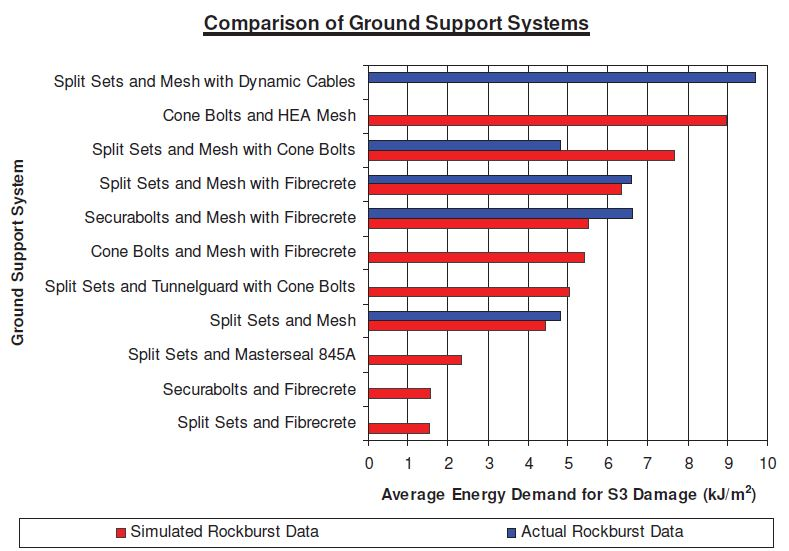
\includegraphics{pics/Heal10.JPG}
    \caption{Comparison of different support systems after \textcite{Heal10}}
    \label{fig:heal10}
\end{figure}
\end{comment}

Reinforcement support, surface support and rock mass form a support system. % that aims to fulfill the previously mentioned support functions. 
As the components work closely together, the support system must be viewed as one unit. There is a lot of interplay between reinforcement and surface support. The energy absorption capacity of a support system is not the sum of the capacity of each individual component. \autocite[1]{Simser07} The capacities for displacement, load and energy absorption must be compatible to ensure the best possible result. \autocite[222]{Kaiser12} 
\textcite[248]{Heal10} stated that: "An ideal integrated ground support system for rockbursting conditions has surface support which is strong enough to transfer load to individual reinforcing elements and engage the full capacity of the rock bolts or cables".
\textcite{Heal10} tested several support systems and evaluated their capacities in real rockbursts. 
%The results are displayed in \autoref{fig:heal10}. The damage level S3 refers to amount of damage a support system can take without rock ejection, which is therefore the level at which the rockburst would not cause any harm to humans present in the area. 
Mesh appears to be necessary to achieve high energy absorption capabilities, without mesh support systems fail at 1,5 - 2 \(\frac{\text{kJ}}{\text{m}^2}\). 
\textcite{Heal10} stated that: "the 1.5 to 2kJ/m\textsuperscript{2} threshold may in fact represents the inherent energy capacity of the unsupported rock mass." which implies that shotcrete alone does not increase the dynamic capabilities of a support system significantly. In order to activate the full potential of the reinforcement support mesh, straps and or lacing are necessary. \autocite[221]{Heal10} 
Shotcrete does stabilise the loose rock around the excavation. For this function a thin layer is enough. \autocite[5]{guler01}
%Lacing increases the energy absorption capabilities of a support system significantly and that chain-link mesh has a higher energy absorption capacity than welded mesh. \autocite{Potvin10} \autocite{canada96} \autocite[575]{sme11}
%Another important factor is bolt plate size, thickness and surface contact as well interaction between plate and washer. 

In burstprone ground a vital task of a support system is dissipating destructive energy, either through deformation, or friction. An important part of a support system are the connections between the different elements. \autocite[2.17]{canada96}\autocite[220]{Kaiser12} A support system will fail when its weakest part fails. Which usually is the reinforcement support. \autocite{Potvin10} \autocite[221]{Kaiser12} 
\autocite[13]{Simser07} If the surface support fails before the reinforcement support, the unbroken bolts remain in the intact rock and are clearly visible. Such a failure mode is called a "naked tendon" failure. \autocite{Potvin10} Such a phenomenon implies the surface support is unable to transfer enough load to the bolts. The loose rock mass detaches itself from bolts during a dynamic event. As the connection between bolt and rock is severed no energy can be transferred, if the surface support does not transfer the energy, the bolts are not loaded. \autocite[7]{guler01} The support system fails at low energy levels, a fraction of its capacity. \autocite[240]{Potvin10}
This is a common phenomenon. Modifying the plates or including straps, lacing or high tensile mesh in the support system can reduce the frequency of this failure mode. \autocite[1]{Simser07} \autocite[240]{Potvin10} 
In order to ensure that the connection between surface support and reinforcement support is strong enough to transfer the impact energy, special attention must be paid to washers, plates and other connective accessories. They should be chosen carefully and thoroughly tested as they often fail in large rockburst events. It´s a known failure mode that bolt nuts simply cut through plates, especially during dynamic events. Thicker and larger plates reduce the frequency of this. \autocite[3]{Simser07}
%An important factor in the effectiveness of surface support is the strength of the connection to the rock mass and the interlink with neighbouring support elements. 
Larger plates help to connect reinforcement support to surface support better.  Welded mesh is susceptible to being damaged by small plates. \autocite[218]{Heal10} Chain-link mesh even more so, as the thinner wires are more easily broken. \autocite{chainlink11}
Another way to handle this is to  put a thin layer of wood or rubber between the plate and the mesh. \autocite[3]{Simser07}
 Lacing is also vulnerable to being damaged by connective elements. It never fails because of rope rupture but instead because the connection elements are the weaker link. \autocite[4.33]{canada96} The strength of lacing therefore is highly dependent on the connective elements (for example: key hole bolts or clamps). If these have sharp edges, lacing ropes might get damaged and fail prematurely. \autocite[3]{guler01} 
%\autocite[221]{Kaiser12} \autocite[129]{chainlink11} Or might damage the surface support. \autocite[218]{Heal10} \autocite[4.33]{canada96} 

Also compatible elements must be chosen to either draw load at the same time or in sequence. For example the maximum deformation of the bolts must fit with the predicted deformation of the rock mass. \autocite[6]{guler01} 

%The sequence of installation of support components is also very important. In order to properly transfer load from the surface support elements to the rock bolts, the bolts must be installed after the surface support elements and with a sufficiently large plates to effectively transfer load. \autocite[4.31]{canada96}

When designing a rock support system in a seismically active mine it is important to keep in mind, what the usual failure modes and their expected severity are and which demands they put on the support system. As well as the constraints put on the support design in order to keep the mine usable. For example what the maximum acceptable displacement is. The rock support system must be able to support the burden of loose rock created through excavation, as well as contain the kinetic energy of ejected rock. It must keep individual rocks from being ejected to protect humans and equipment and finally minimize the inward movement of rock face in total and therefore loss of excavation space. \autocite[4.35]{canada96}
Based on these considerations support elements must be chosen which either are able to prevent the initiation of damage or control the the failure process. \autocite[223]{Kaiser12} 

\textcite[2.8]{canada96} put it this way: 
\begin{quote}\textit{''An ideal support system must either be strong enough to suppress this volume increase or it must have sufficient ductility to allow the volume increase to take place  without destruction of the support system''}
\end{quote} This quote defines the basic approach behind surface support in seismically active mines. Either the support must sufficiently strong to take the load, or it must be flexible enough to deform without destruction. 

In the first case a support system must be strong and provide enough support to keep the rock mass from unravelling. This usually involves using lots of shotcrete. If the demand of the rock on the support system increases, it may not be economically viable to provide the amount of support needed to avoid failure. In this case a different strategy adopted. Soft rock support can be used, which is able to "yield". This means that it has to be able to deform sufficiently to dissipate the energy of an dynamic event. \autocite[220]{Kaiser12} Such a support systems usually include chain-link and lacing. As \textcite[220]{Kaiser12} put it: "A yielding rock support system is a system in harmony with its surrounding, failing rock mass." At the same time, the displacement of the rock support system should be low enough that it is still able to hold the broken rock, produced by the unravelling rock mass, after the seismic event has ended. The larger the displacement the larger the amount of loose rock around the excavation becomes and the more load is put on the surface support.\autocite[7]{villa13} 
After a dynamic event has occurred and the dynamic stresses have dissipated, the static stresses still remain. This means that even after deforming significantly under the dynamic stress
%The support system must retain enough post-peak strength to be able to prevent gravity driven failure of the now loose rock mass after quasi static conditions return. Which means that 
the rock support has to maintain its load carrying capacities. % even after sustaining large deformations. 
\autocite[77]{Heal10}
\textcite[13]{Simser07} advocated a hybrid system of stiff arches and yielding elements in very vulnerable areas.

%"give" under the dynamic load but still be able to function as quasi static support. 
 
%While deformations and associated loss of excavation space are less than ideal they sometimes can not be avoided. %It is acceptable and expected that rock support only survives one large seismic event and needs maintenance afterwards in order to be able withstand the next one.

\section{Factor of Safety}

In order to quantify the likelihood that a given system is going to fail a probability factor can be defined.
Usually this is called the Factor of Safety (FoS) which is defined as displayed in \autoref{equ:FoS} \autocite[3.15]{canada96}.

\begin{equation}
\label{equ:FoS}
FoS = \frac{Capacity}{Demand}
\end{equation}

%\textcite[573]{Masoudi18} states in regard to rockbursts that: 
%"Ground energy demand cannot accurately be determined or calculated." 
%Because the severity and frequency of rock bursts is influenced by several factors, such as: size and geometry of excavation, rockmass properties, \textit{in - situ} stresses and their orientation, distance and energy levels of seismic source, stress wave magnification, support system properties and interplay of these factors. 

The destructive effects caused by different kinds of rockbursts vary strongly, as they are dependant on a number of different factors. The frequency and severity of rockbursts is hard to predict as well. Therefore the demand of the rock mass can not be globally defined. \autocite[8.6]{canada96}
The capacity of rock support must be assessed in terms of energy absorption, displacement and load. \autocite[221]{Kaiser12} 
A support system has to be tailor made for each mine, if not each area of a mine, as local conditions will heavily influence how burst prone the rock mass is. Designing a rock support system is an involved and difficult process that has to deal with ever changing parameters. It has to be adaptable and creative. \autocite[223]{Kaiser12} For this reason \textcite[216]{Kaiser12} described designing a dynamic rock support system as: "interactive and iterative process of selecting proper support elements to form a rock support system which has enough capacity to meet the expected demands" Which means that a design concept has to be modifiable and needs to be adapted to the conditions encountered \textit{in - situ}.

%Usually the reinforcement support is activated by displacement of surface support elements.
%Problems can arise when unyielding bolts are combined with soft surface support, like chain-link mesh. Chain-link requires large displacements before it starts to absorb energy. For example grouted bolts have a displacement limit of 10 - 30 mm, while chain-link mesh´s energy absorbtion capacities are only activated at approximately 100 mm. \autocite[2.20~-~2.22]{canada96} Which means that in this system the reinforcement support has already failed by the time the surface support springs into action. Therefore it is necessary to carefully design support systems in order to maximize synergy.

%''burst control then essentially consists in avoiding or reducing the build-up of such stresses from the beginning'' \autocite[25]{Brauner94} 

\section{Seismic Risk}

Accordingly \textcite{Heal10} suggested a different approach, that takes into account the different needs of different areas of the mine.\textcite{Heal10} coined the term "seismic risk". Seismic risk can be calculated for an arbitrarily small block inside of a mine. It is defined as:
\begin{equation*}
    Seismic~Risk =  Seismic~Hazard * Excavation ~Vulnerability * Exposure
\end{equation*}

The seismic hazard is largely dependent on the expected peak particle velocity PPV. PPV is a function of the distance from the event to the location, as well as the magnitude of an event. The seismic hazard is also influenced by the frequency of seismic events.
The excavation vulnerability depends on the span of the excavation, the deployed ground support system, the ratio of \(\sigma_1\) to the uniaxial compressive strength UCS of the rock mass and the presence of geological structures.
Exposure is defined as the probability of humans being in the area at any given point in time.

As the seismic risk can be calculated for arbitrarily small block of the mine, high risk areas can be identified, and additional measures deployed.

\chapter{Testing Dynamic Rock Support}

In order to choose fitting components for a rock support system it is necessary to gather quantitative data about their properties and not just to rely on experience and empirical data. In case of seismically active mines, the energy absorption capabilities and displacement rates under dynamic load are of particular interest. Materials tend to display higher UCS the faster load is applied \autocite[4.28]{canada96}, therefore normal laboratory tests tend to heavily underestimate the capabilities of rock support systems under dynamic loading conditions. But dynamic loading conditions are difficult to replicate in laboratory settings, and there are no standardized tests. Past events are therefore a valuable source of information.

\section{Back Calculations}

Back calculations look at past rock bursts and try to understand the failure mechanism of the support and correlate the stresses in the rock support to the magnitude of the seismic event. \autocite{Potvin10} With this data the demand of the rock mass is calculated. Predictions of future rock bursts and identifying burst prone areas are part of back calculations. \autocite{Heal10} The next step is to try and replicate the observed failure modes \textit{in - situ}.

\section{Blast Tests}

For this purpose the support system, which is supposed to be tested, is deployed in a section of the mine. A rockburst is simulated by blasting the rock behind the rock support. \autocite[98]{Heal10}
%A blast test is run by deploying the support system, which is intended to be tested in a section of the mine and afterwards simulating a rockburst through blasting. \autocite[98]{Heal10} 
 The wave length and frequencies caused by blasting are different from natural seismic events. Blast tests test the entire support system and the interplay of its components \textit{in - situ}. \autocite[243]{Potvin10} \textcite{shirzadegan16} conducted blast tests at Kiirunvaara mine.
As this kind of test is hard to repeat it is important to get it right the first time. Which means, as much data as possible must be captured in a quantitative fashion. Also the unwanted effects of expanding gases, which are not present in real rockbursts, must be minimized. \autocite[98]{Heal10}
This kind of test is very cost intensive and has limited repeatability.

\section{Drop Tests}
\label{sec:droptest}

To test large numbers of different configurations the repeatability of the test has to be increased while the cost per test must be decreased. For this purpose drop tests can be used.
Drop tests usually consist of a drop weight, that is lifted above the specimen and then dropped on it. The weight is usually accelerated by gravity. The specimen can be a single rock bolt or a surface support element or an combination of support elements or a complete surface support system consisting of bolts and surface support. This kind of test is cheap to run, after an initial high setup cost and has very good repeatability. \autocite{Potvin10} \autocite[84]{Heal10}

Differences between tests and \textit{in - situ} conditions are many fold: rate of loading, stiffness of the testing system, interaction between rock and support system from adhesion and/or friction among other factors. \autocite[35]{Brauner94} The loading mechanism can differ greatly from what would be induced by a seismic event. \autocite[84]{Heal10}

Also drop tests have limitations that influence the response of support elements. Especially the boundary conditions are difficult to simulate. Shotcrete or mesh would usually be connected on all sides, but specimen size is limited. \textcite{Robert19} constructed a very large rig with a possible sample size of 5 x 5 m for this purpose. It is quasi-static and a hydraulic jack with a maximum force of 200 kN and maximum displacement of 1200 mm is used. \textcite{Robert19} found that reinforced boundaries increased in the load capabilities of chain-link dramatically. The importance of controlling the boundary conditions when testing mesh can not be overstated. 
If no further steps are taken, tests are conducted with open boundaries, which is entirely different from the conditions in reality. According to \Textcite[243]{Potvin10} FRS performs much better during impact tests than during blast tests for unknown reasons, possibly connected to similar phenomena.

Therefore such tests can only provide estimates of the properties of rock support elements and should mostly be viewed as a way to compare various support systems. \autocite{Potvin10} \textcite[13]{Simser07} states: "Laboratory testing may never duplicate the intricacies of an actual rockburst but can provide repeatable and reliable insight into how support systems behave under dynamic loads."

Drop tests can be divided into two categories: during type 1 tests one high energy drop per sample is performed and therefore these kind of tests determine the maximum energy the support energy can survive in one large event. Type 2 testing utilises several low energy drops on one specimen. It is not uncommon during type two tests that drops are repeated until the sample breaks and that amount of drops the sample survives is also used as information. Type 2 therefore measures the capability of the support to withstand several smaller events. 

Several drop test rigs that have been constructed that fit into these categories.
%There have been several different drop test rigs constructed in the past. %As most severe rockbursts at Kiirunavaara mine are linked to large seismic events, the tests in this thesis were designed following the design paradigms behind test type 1. %As soon as a support system with sufficient energy absorption capabilities has been designed, its fatigue resistance becomes interesting. But at this point in time a satisfactory rock support system for Kiirunavaara mine is still under development

\chapter{Literature review of drop test facilities}

In \autoref{tab:drop} an overview of the specifications of various dynamic and static test rigs are given. 

\begin{table}[h!]
    \centering
    \begin{tabular}{*{6}{l}}
    \toprule
    name & year& max velocity & max drop height & max drop weight \\
    && \(\rfrac{m}{s}\) &  m & kg \\
\midrule
    SIMRAC      & 1996 & 9      & 4,0   & 565       \\
    GAP6111     & 1999 & 8      & 3,0   & 10.000    \\
    GAP616      & 2001  & 3     & 0,5   & 1.000     \\
    WASM Bolt   & 2004 & 6      & 2,0   & 2.000     \\
    WASM Mesh   & 2012 & 6      & 2,0   & 2.000     \\
    NIOSH       & 2017 & 7      & 2,5   & 200       \\
    \end{tabular}
    \caption{Overview of different drop test rigs}
    \label{tab:drop}
\end{table}

\section{SIMRAC Dynamic Stope Test Facility}

\begin{figure}
\centering
\begin{tikzpicture}
% canadian rock burst drop rig 


\draw[thick] (0,0) -- (10,0) -- (10,6) -- (0,6) -- cycle;
\draw[thick] (1,1) circle [radius=0.15] % pressure points
(5,1) circle [radius=0.15] 
(9,1) circle [radius=0.15] 
(3,3) circle [radius=0.15] 
(7,3) circle [radius=0.15] 
(1,5) circle [radius=0.15] 
(2,4.5) node[align=left, below] {support column}
(5,5) circle [radius=0.15] 
(9,5) circle [radius=0.15];
%[thick] (4.5,2.5)  rectangle (5.5,3.5)
\draw[thick, fill=lightgray] (5,3) circle [radius=0.5];
\draw (5,2) node[align=center] {impact zone}
(3,1) node[align=center,above] {1,2 m};
\draw [<->] (1.5,1) --+ (3,0);
\end{tikzpicture}

\caption{Impact test setup as described by \\ \textcite{canada96}}
\label{fig:can}
\end{figure}

\Textcite[4.24]{canada96} conducted so called "impact tests". 
The experiments were set up in the following fashion:

A weight of 565 kg was dropped on reinforced shotcrete panels measuring 1,5 x 2,75 m, supported on 8 points by dummy bolts, each fitted with a loading cell. The bolts were laid out in a 1,2 x 1,2 diamond pattern.  In \autoref{fig:can} a schematic of the setup is displayed. The maximum drop height was 4 m. The drop weight hit the reinforced shotcrete directly. The drop weight had cylindrical shape, with a diameter of 0,6 m and a hole through the middle for the guidance system.
The results were an approximate linear correlation between impact energy and deformation, with the panels being able to absorb about 15 \(\frac{\text{kJ}}{\text{m}^2}\) and still being functional as static support afterwards.

\section{GAP 611}

\begin{figure}
    \centering
    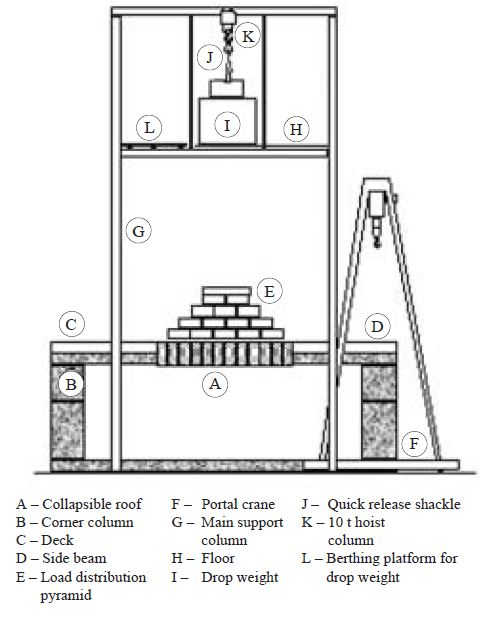
\includegraphics{pics/GAP611_side.JPG}
    \caption{Sideview of GAP611 after \autocite{human04}}
    \label{fig:gap611}
\end{figure}

This facility was built by SIMRAC in 1999 in South Africa. The general set up is displayed in \autoref{fig:gap611}.
The testable area of support is 3 x 3 m. Concrete blocks are placed on the support which simulated the hanging wall. They can move independently of each other. The drop weights hits the simulated hanging wall and the energy is transferred to the support system. \autocite{human04}


\section{GAP 616}

This rig was originally built by SRK consulting and was modified by the Safety in Mines Research Advisory Committee to be able to test more than FRS. The rock mass is represented by concrete bricks. The reason being, that the failure plane between the brick would be vertical. The drops were repeated at the same energy level and height until failure of the system. The concrete was sprayed directly on one layer of the bricks. 


\section{West Australian School of Mines}

\begin{figure}
    \centering
    
\subcaptionbox{Test rig for dynamic tests on bolts\label{fig:WASMbolt}}{
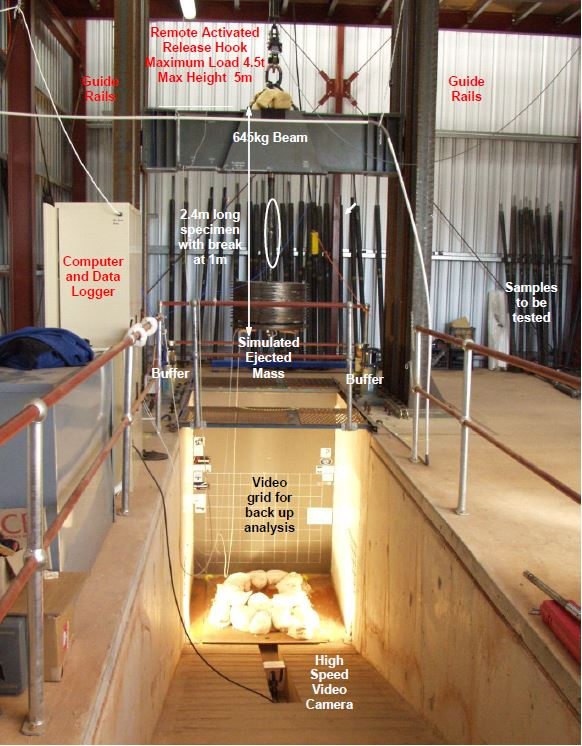
\includegraphics[width=0.45 \linewidth]{pics/WASMbolt.JPG}
}
\subcaptionbox{Test rig for static testing of mesh \label{fig:WASMstatmesh}}{
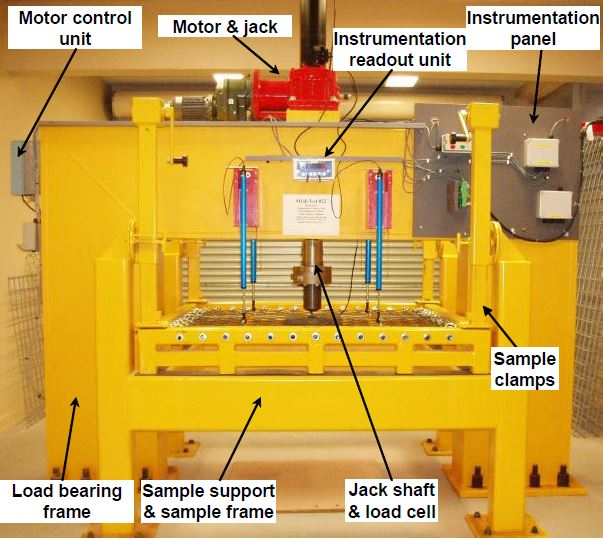
\includegraphics[width=0.45 \linewidth]{pics/WASMstatic.JPG}
}
\subcaptionbox{Test rig for dynamic tests of mesh, note the variable boundary conditions \label{fig:WASMdynmesh}}{
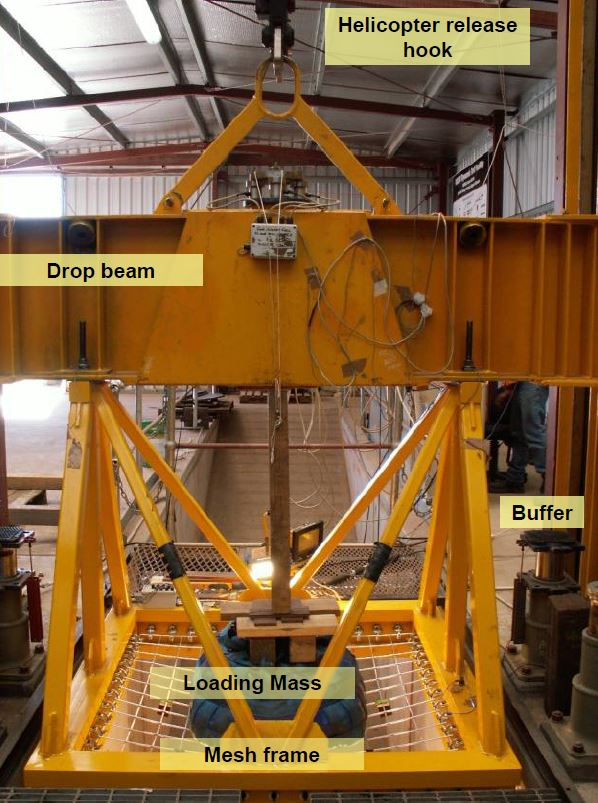
\includegraphics[width = 0.45 \linewidth]{pics/WASMmesh}
}

\caption{Tests rigs built by WASM after \textcite{villa09}}
\end{figure}

The Western Australian School of Mines (WASM) built several dynamic and static testing facilities for testing ground support. The drop test facility uses a different way of transferring load. Instead of dropping a weight on the static support, the support elements and weight are dropped together and slowed by buffers and the energy is transferred during that deceleration. It´s called momentum transfer and is supposed to more closely resemble \textit{in - situ} conditions. Most of their facilities were built in 2004. They built a drop tests rig for bolts (see \autoref{fig:WASMbolt}) a static test rig for mesh, with an very elegant solution to the boundary conditions problem (see \autoref{fig:WASMstatmesh}) a dynamic rig for mesh and concrete panels (see \autoref{fig:WASMdynmesh}).
%As of now it is not possible to test concrete samples with any of their rigs.

\section{NIOSH}

\textcite{Raffaldi17} described the test facilities built by 
the National Institute for Occupational Safety and Health Spokane Mining Research
Division in Spokane, Washington, United States of America. It is a quasi-static and a dynamic testing facility for ground support. The dynamic facility utilises momentum transfer. Only concrete samples can be tested. Mesh can only be used as reinforcement. One type of TSL has been tested. 



%TO DO more test methods!

%\subsubsection{Drop Test}


Building on these machines and the results of their drop tests a drop test rig was developed at Kiirunvaara mine. It was designed with the needs of the mine in mind.

\chapter{Kiirunavaara}

The Kiirunavaara mine located in Kiruna, Sweden and operated by LKAB has struggled with rockbursts since 2008 \autocite[5]{Krekula17}. It is a large underground iron ore mine, with an annual production of 27,5 Mio t crude iron ore in 2018. \autocite[28]{LKABfinance} 
The orebody consists mostly of magnetite.
In \autoref{fig:geo} a map of the geology of the area is given.
%As displayed in \autoref{fig:geo} the ore at Kiirunavaara is mostly magnetite.
It is mined using sub level caving. The current production depth is at around 1100 m.%, the ore body is estimated to continue to depths of 2000 m. %With increasing depth the tensions inside the the rock mass increase as well and the ground becomes more burstprone. Therefore the support systems needs constant updating and development.

%The next step LKAB wants to take is optimizing its surface support concept. The chosen method are drop tests. Drop testing works utilizing gravity to either directly or indirectly transfer kinetic energy to isolated surface support elements. \autocite[1]{Potvin10} Which means that drop weights are dropped from fixed heights onto surface support elements and the mode of failure of these elements together with their maximum capacities among other measured values are studied to gleam insights to help to iterate towards an compromise between rigidity and derformability.
%Drop tests are easily replicable, the largest amount of work is building and handling the test panels. Therefore they are a cheap way to test various set ups. But drop tests have their draw backs. It is only possible to test reinforcement elements, therefore the interaction between surface support and reinforcement support and rock face can not be investigated. The surface support activates the reinforcement support through their connection, insufficient activation of the reinforcement means unused potential, unnecessary cost and premature failure. Overall they are a practical way to optimize surface support under dynamic loading conditions.

\begin{figure}
\centering
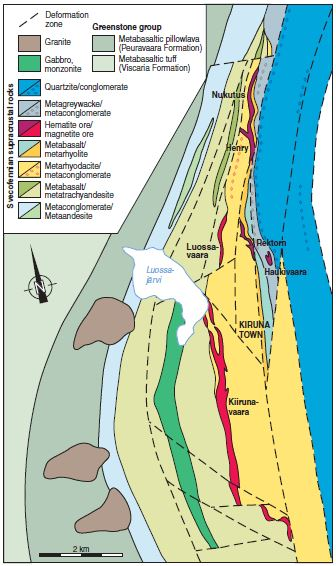
\includegraphics[height = 0.5\textheight]{pics/geo.jpg}
\caption{Geology of the Kirunavaara area \autocite{KirunaGeo}}
\label{fig:geo}
\end{figure}

\section{Transition from Seismically Inactive to Seismically Active}

Up until 2007 only minor rockbursts happened at Kiirunavaara mine which were also confined to a small area within the mine. After 4 large seismic events and corresponding rockbursts on 2 to 3 levels between late 2007 and early 2008 it became obvious that rockbursts were no longer exceptions. %To understand the problem a network of geophones was built, as displayed in \autoref{fig:phone} the amount of geophones increased substantially. \autocite{dahner12}

\begin{comment}
\begin{figure}
    \centering
    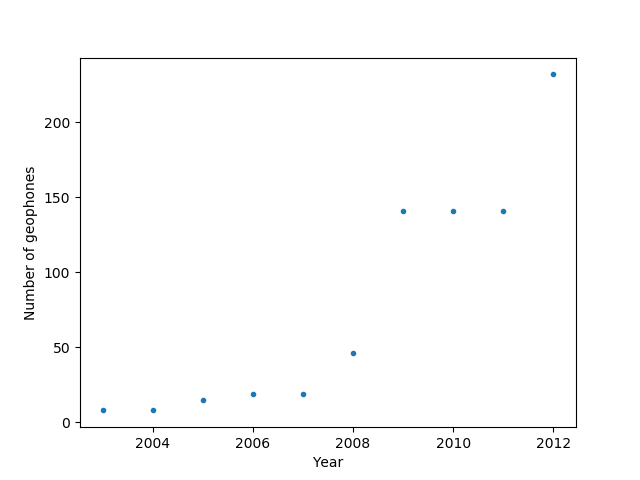
\includegraphics{pics/geophones.png}
    \caption{Increase in number of active geophones between 2004 and 2012 after \autocite[4]{dahner12}}
    \label{fig:phone}
\end{figure}
\end{comment}

Measures to decrease the vulnerability to rock bursts were taken. For example the production sequence was optimised and procedures to close vulnerable areas of the mine were implemented.
The rock support system used so far only had to provide static support, it consisted mostly of 3 - 4 cm of shotcrete and grouted rebar. \autocite[9]{dahner12}

\section{Current Support System}

\begin{figure}
    \centering
    \begin{tikzpicture}
%current support system

%membrane
\draw (0,0) arc [radius = 8cm, start angle= 120, end angle= 60];
\draw (0,-1) arc [radius = 8cm, start angle= 120, end angle= 60];
\draw [thick,dash pattern={on 7pt off 2pt on 1pt off 3pt}] (0,-1.3) arc [radius = 8cm, start angle= 120, end angle= 60];
\path (0,-1.8) arc [radius = 8cm, start angle= 120, end angle= 60] 
coordinate [pos = 0.2] (left)
coordinate [pos = 0.35] (leftmid)
coordinate [pos = 0.5] (mid)
coordinate [pos = 0.65] (rightmid)
coordinate [pos = 0.8] (right);

%bolts
\draw 
(left) -- ++ (110:4)
(leftmid) -- ++ (100:10)
(mid) -- ++ (90:4)
(rightmid) -- ++ (80:10)
(right) -- ++ (70:4);

%text
\node[right] at (8.5,0.5) {rock};

\node[right] at (8.5,-0.5) {FRS};

\node[right] at (8.5,-1.3) {welded mesh};

\node at (4,-1.8) {excavation};

\node at (4,7) {cable bolts};

\node at (7,3) [right] {dynamic bolts};
\end{tikzpicture}
    \caption{Cross section of the current support system}
    \label{fig:cross}
\end{figure}

\begin{figure}
    \centering
    \begin{tikzpicture}

%drift
\draw (0,0) -- (0,2) -- (2,2);
%\draw (-1,0) -- (-1,2) -- (-3,2);
\draw (2,3) -- (0,3) -- (0,5);
%\draw (-3,3) -- (-1,3) -- (-1,5);
\draw (-1,0) -- (-1,5);

%rock
\path [fill = lightgray]
(0,0) -| (2,2) -| cycle
(2,3) -| (0,5) -| cycle
(-1.5,0) -| (-1,5) -| cycle; 

%cable bolts
\foreach \x in {0.1,0.2,...,0.9}{
\foreach \y in {0.1,0.2,...,0.9}{
\draw[fill = black] 
(-1+\y,2+\x) circle [radius=0.01]
;}}

%shotcrete arch
\draw (0,0.5) to [bend right](-1,0.5)
(0,0.4) to [bend right](-1,0.4);
\draw (0,1.3) to [bend right](-1,1.3)
(0,1.4) to [bend right](-1,1.4);

\draw (0,4.5) to [bend right](-1,4.5)
(0,4.4) to [bend right](-1,4.4);
\draw (0,3.5) to [bend right](-1,3.5)
(0,3.4) to [bend right](-1,3.4);

\draw (1.5,2) to [bend left](1.5,3)
(1.6,2) to [bend left](1.6,3);
\draw (0.7,2) to [bend left](0.7,3)
(0.6,2) to [bend left](0.6,3);

%text
\node at (1,1) {rock};
\node at (1,4) {rock};
\node at (2.5,2.5) {drift};
\node [left] at (-1.5,2.5) {cable bolts};
\node [left] at (-1.5,0.9) {shotcrete arch};
\node [left] at (-1.5,3.9) {shotcrete arch};

%\node [right] at (0,3.5) {cable bolts};
%\node [right] at (0,1) {shotcrete arch};
%\node [right] at (-3,2.5) {drift};
\end{tikzpicture}
    \caption{Top view of the placement of shotcrete arches and cable bolts}
    \label{fig:arch}
\end{figure}

The support system developed in response to Kiirunavaara mine becoming seismically active has evolved and solidified into the support system currently in use. It consists mainly of 10 cm of fibre reinforced shotcrete, with welded mesh on top with a wire diameter of \o 5,5 mm and and an aperture of 75 mm and 3 m long dynamic bolts with 1 m spacing and > 7 m long cable bolts in the roof of 3 - way and 4 - way intersections or where the geology requires it. See \autoref{fig:cross}.  Especially burst prone areas are supported with concrete arches with a thickness of 200 mm. The bolts are square spaced and mesh is connected with 3 squares of overlap. % as displayed in \autoref{fig:mesh}.
Pillars between ore passes are reinforced with steel straps called "Fjällband" if the operational rock mechanic engineers recommend it. \autocite{Jonson15}
%%%% maybe fix that sentence?

\section{Requirements of Support System}
This support system and any change made to it have to fulfill several requirements.

\subsection{Lifetime}

The most important one is longevity. A support system has to be serviceable for as long as the excavation is expected to be open. See \autoref{tab:life}. Please note that active production area refers to drifts with ongoing production and that support used in the primary infrastructure must always undergo long-term tests. After the times mentioned the support system has to retain 85 \% of the initial strength requirements. \autocite[3]{Winsa18}

\begin{table}
    \centering
    \begin{tabular}{ll}
    \toprule
        Type of use & Lifetime in years \\
    \midrule
         Production area & 10  \\
         Active production area & 2 \\
         Main haulage level & 20 \\
    \bottomrule
    \end{tabular}
    \caption{Approximate lifetime expectation at Kiirunavaara Mine after \textcite[3]{Winsa18}}
    \label{tab:life}
\end{table}

\subsection{Surface Support}

%The strength requirements for surface support are entirely based on quasi-static tests. 
The quasi static strength of FRS is tested and evaluated using \autocite{c1550}. 
For mesh only welded mesh has a regulated testing procedure.
The dynamic capabilities are assumed based on \textcite{Potvin10}.
Blast tests conducted by \autocite[9]{shirzadegan16} give an energy absorption capacity of 4 \(\frac{\text{kJ}}{\text{m}^2}\) for this combination.
%The energy absorption of FRS and mesh are assumed to be 7,5 and 2,5 \(\frac{\text{kJ}}{\text{m}^2}\). After a simple addition that means that the current support system supposedly has energy absorption capabilities of 10 \(\frac{\text{kJ}}{\text{m}^2}\). \autocite[4]{Biruk13}

\subsection{Reinforcement Support}

For bolts a mix of static and dynamic tests are required. These are conducted by CanmetMINING. \autocite{Winsa18}

\chapter{Tested Material}

With the requirements discussed in the previous chapter in mind the material that would be tested were chosen.

%%%%%%%%%%%%%%%
%Concrete
\section*{Concrete}
%TO DO more concrete information
The concrete used in the tested sample %was almost exclusively 
fibre reinforced with approximately 40 \(\frac{\text{kg}}{\text{m}^3}\) of steel fibres. Its hardness class was C50, it has a UCS of 50 MPa.

%Its cement was produced by X

%The aggregates are sourced from Y.

%%%%%
%Mesh
\section*{Welded Mesh}
The welded mesh has a wire diameter of \o 5,5 mm and c/c 75 mm. It is used in 2,2 on 2,3 m sheets. 

\section*{Textile Mesh}
The textile mesh that was be tested is manufactured by Huesker and is called minegrid. 

%%%%%%%%
\section*{Chain-Link Mesh}

Special attention has to be given to the plates used with chain-link mesh. As the wire are quite thin, they are prone to breaking when used in conjunction with a flat plate. \textcite{chainlink11} suggests using special spiked plates.
%As the number of available samples was quite small, chain-link mesh will not be tested.

%%%%%%%%%%%%%%
\section*{Fjällband}
\label{sec:fjäll}

\begin{figure}
    \centering
    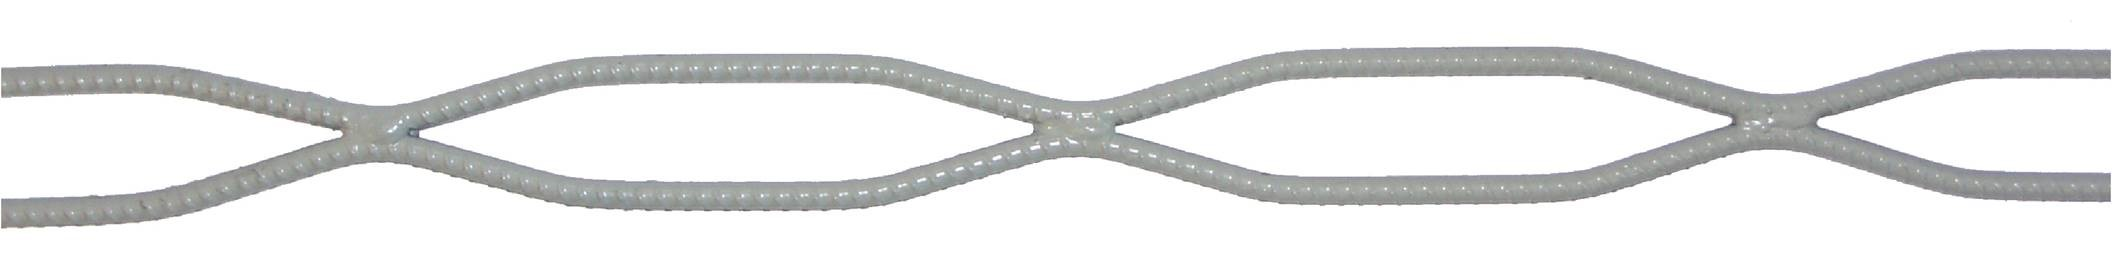
\includegraphics[width=0.95\linewidth]{pics/Fjallband.jpg}
    \caption{A sketch of Fjällband}
    \label{fig:fjäll}
\end{figure}

Fjällband is a type of strap. It is manufactured in-house and has to be installed manually which is time and cost intensive. Its effects on the rock support have not been studied so far. It consists of two wavy metal rods that are welded together at their peaks, see \autoref{fig:fjäll}.  %implementing a different type of lacing which could be installed in at least a mechanised if not automized way would be more efficient. 

%%%%%%%%%%%%%%%
%Lacing
\section*{Lacing}
Only wire rope will be tested, though it might be interesting to consider rope made from nylon or polyester in the future. Of course the diameter and the deformability would increase but it would be lighter, easier to handle and would not suffer corrosion. Fire might pose a large risk to synthetic rope. If lacing were to be deployed across large areas in the mine it might be worth considering "exotic" materials, such as nylon or polyester. Umeå university and LKAB started  a joint project to investigate using synthetic materials for hoist cables instead of steel. The results of this project were not available when the test matrix of this thesis was planned.
The results from these investigations could be used for future tests. %It has not yet been tested.
For the current experiments galvanized steel wire (6 x 24 + 7FC) was used. It had a breaking load of 43.9 kN. The technical data sheet can be found in the appendix.

%%%%%%%
\section*{Connective Elements}
The bolts were made from M30 threaded rods. The bolt plates that will be used in the large scale sample tests are the same as are used underground.
When testing chain-link or textile mesh some sort of cushion will need to be put under the bolt plate.

The samples that were used in the drop tests tried to include as much of the current system as possible while also experimenting with other options.

\chapter{Testrig}
%In this chapter I will describe the test rig, the test method, why it was chosen, what its limits are, how it works behind the scenes (mechanically/dynamically) how the tests are set up and so on.

%\begin{comment}  


\begin{figure}
\centering
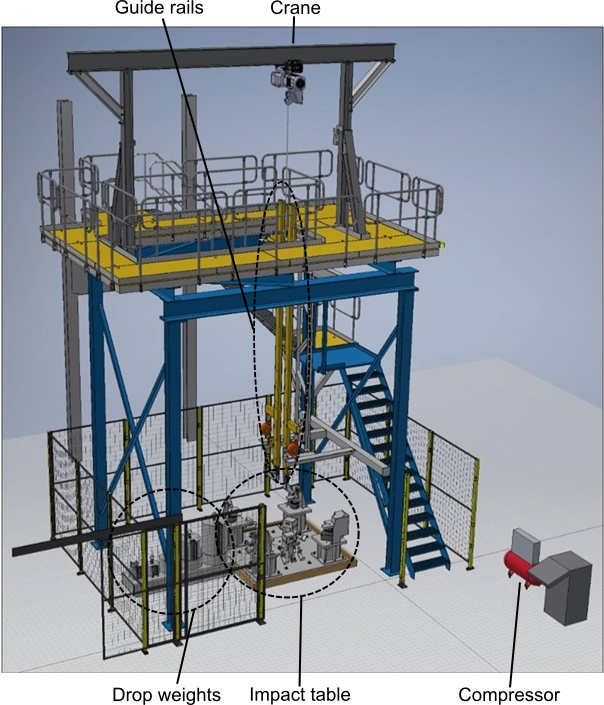
\includegraphics[width=\linewidth]{./pics/rig.png}
\caption{Drop test facility used at Kiirunavaara Mine}
\label{fig:drop}
\end{figure}

If you build a race track from scratch then drive a few laps on it and check the times, you have no idea if the car you're using is fast or slow. You need more data. As soon as you have driven a second car around the track you know which of the two is faster. The more cars you drive around the track the better your understanding of the capabilities of different cars ant the track itself becomes. 
It is the same for rock support systems and drop test rigs.

There is a lot of data available in literature, giving a general guideline of what to expect when running tests on various materials. But the test rig constructed at Kiirunavaara Mine is unique. Of course the results should be comparable to the results of other test rigs but they will be ever so slightly different.

To gain a baseline of the capabilities of the current support system and develop the test rig to its full potential is the aim of this thesis. With this baseline it is possible to compare future developments and ideas to the status quo and decide whether they are worth exploring further.  

The current test rig is depicted in \autoref{fig:drop}. As these were the first serious tests run with the rig, the setup and sensor array underwent some changes. Further enhancements are always possible, some are already planned, more will be discussed in the course of this thesis and the current setup is just a stepping stone on the way to a fully fledged testing facility. 

It is designed to test panels with dimensions of either as a circular plate with 0,8 m diameter or a square plate with 1,5 x 1,5 m. The impact energy can vary from 0 to almost 40 kJ. It is gravity based, which means the impact weight is in free fall. There's no direct measurement of the impact velocity. As the drop height is relatively low, < 4 m, air resistance negligible. The drop weight is supported by guide rails in order to hit the specimen in the center, the drop weights are fitted with low friction material. Currently there is no direct way to measure impact velocity, it is instead calculated, as per industry standard \autocite[13]{Crompton18}. %The impact energy is also only calculated. %TO DO fix energy calculation

\section{Energy Level}

The first challenge when testing the round samples was determining the energy level at which the specimen would crack but not break. The round concrete samples had a large variation in properties which made estimating the survivable impact energy even more interesting. %It did not seem sensible to calculate the energy needed through computer assisted means nor to spend hours trying to solve it analytically. 
This was done through trial and error. A question that posed itself during this process was turning the qualitative analysis of the destruction of the test samples, through visual inspection, into comparable numbers. 
\Textcite{canada96} divides broken samples into 4 categories. This categorisation was based on visual inspection of the post - test samples.

\begin{itemize}
    \item mild damage
    \item moderate damage
    \item severe damage
    \item destroyed
\end{itemize}

%Adopting this system seemed sensible, but as the tested specimen were all very homogeneous it was possible to implement a more quantitative system, based on the amount and width of cracks. 

\begin{figure}
    \centering
    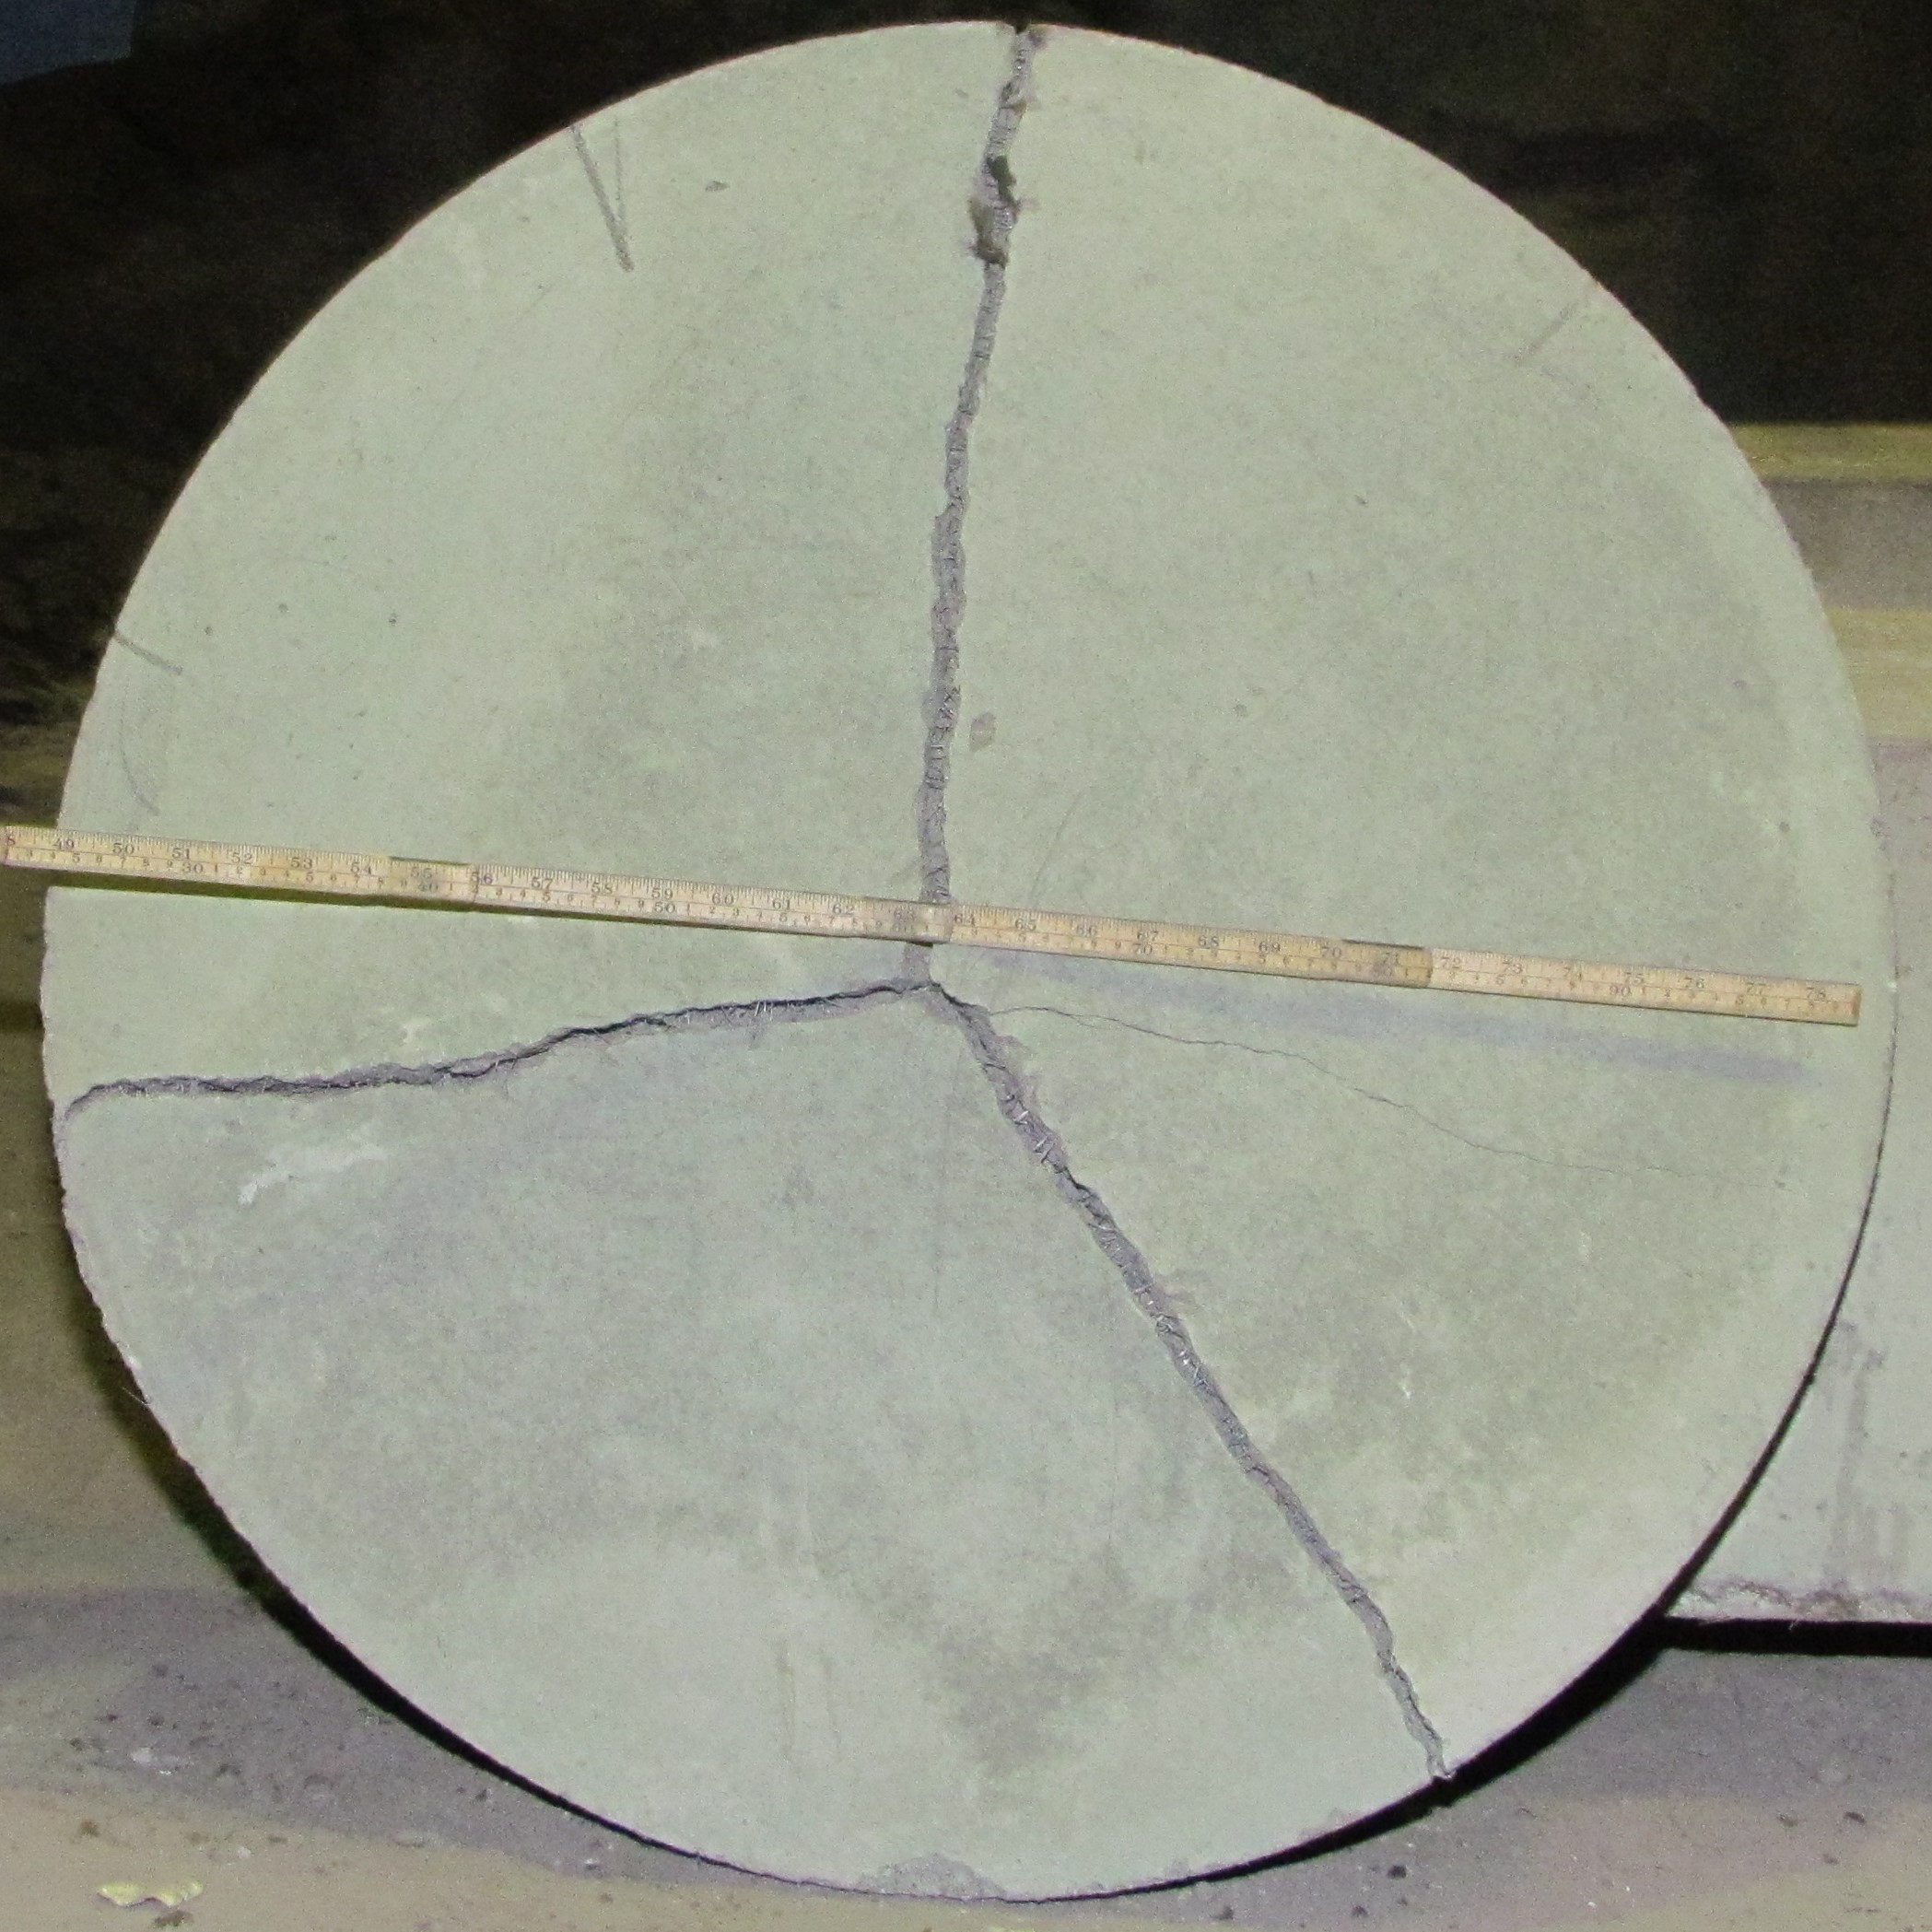
\includegraphics[width = 0.45 \linewidth]{appendix/2018-12-04_Rfrs_50_0,3.JPG}
    \caption{Crack pattern}
    \label{fig:crack_pattern}
\end{figure}

This system is qualitative and the measured results are influenced by the observer. A cautious operator might rate a sample as severely damaged, while a more confident observer could rate it as moderately damaged, for example. Therefore a more quantitative system was implemented.
As most of the energy is absorbed by forming cracks, the width of each crack was measured in 2 to 3 places and averaged. The length of the cracks was also recorded. From the crack length and width the surface of each crack could be calculated and therefore the entire crack surface of each specimen. For the round samples the most common failure mode was 3 large cracks (> 10 mm) accompanied by one or two small cracks (< 1 mm). See \autoref{fig:crack_pattern} or Appendix.

The median crack width was used to calculated the crack opening angle, to minimize distortion through outliers. The crack opening angle \(\Theta\) is defined as displayed in \autoref{fig:crack}. \(\Theta\) was calculated using \autoref{eq:theta}.

\begin{equation}\label{eq:theta}
    \Theta = 2 * \arctan{ \frac{width ~of~the~crack}{2 * thickness~of~the~panel}}
\end{equation}

\begin{figure}
\centering
\begin{tikzpicture}
%Crack angle stuff

\draw (6,0) coordinate (right);
\draw (4,0) coordinate (left);
\draw (5,5) coordinate (root);
\draw [thick] (0,5) -- (10,5)
(0,0) -- (left)
(right) -- (10,0);
% jagged cracks
\draw[thick]
(right)
-- ++(0.1,0.5)  
-- ++ (-0.1,0.2)
-- ++ (0.2, 0.1)
-- ++ (-0.2,0.1)
-- ++ (-0.1,0.8)
-- ++ (0.1, 0.2)
-- ++ (0.2, 0.2)
-- ++(-0.3, 0.3)
-- ++ (-0.1 , 0.4)
-- ++ (0.0, 0.3)
-- ++ (-0.3 , 0.4)
-- ++ (-0.2,0.4)
-- ++ (-0.2, 0.3) % end point
-- ++ (-0.3, -0.5)
-- ++ (-0.4, -0.2)
-- ++ (-0.2, -0.4)
-- ++ (0.1, -0.3)
-- ++ (0.1, -0.1)
-- ++ (-0.2, -0.4)
-- ++ (-0.4, -0.3)
-- ++ (0.1, -0.5)
-- ++ (-0.1,-0.2)
-- ++ (-0.3,-0.1)
-- ++ (0.2,-0.2)
-- ++ (0.1,-0.5)
-- (left)
;
\draw [gray]%[thick, dashed, red] %virtual crack 
(left) -- (root.south) 
coordinate[near start] (lmid)
-- (right) 
 ;
\draw [{Latex[length=3mm, width=1mm]}-{Latex[length=3mm, width=1mm]}] (4,-1) -- (6, -1)
node[midway, above]{width of crack};

%\draw [{Latex[length=3mm, width=1mm]}-{Latex[length=3mm, width=1mm]}] (lmid) arc [radius = 3.85, start angle = -101.31, delta angle = 22.62]
%node [midway, below] {\(\Theta\)} ;

% Draw the arc which center is (2,1)
\draw [{Latex[length=3mm, width=1mm]}-{Latex[length=3mm, width=1mm]}] ([shift=(-101.31:4cm)]root) arc [radius = 4cm, start angle = -101.31, delta angle = 22.62] node [midway, below] {\(\Theta\)} ;

\draw [{Latex[length=3mm, width=1mm]}-{Latex[length=3mm, width=1mm]}] (8,0) -- (8,5) 
node [midway, sloped, above] {thickness of the panel};


\end{tikzpicture}
\caption{Crack opening angle}
\label{fig:crack}
\end{figure}

%The energy absorbed by support elements was defined as the area underneath the force/displacement curve. 

\section{Failure Criteria}
Another problem was defining the failure criteria. \textcite{canada96} stated that rock support must be able to withstand quasi static loading conditions after a dynamic event.  %The construction of a quasi-static test rig is planned. The intend is 
For this a quasi-static test conducted with the same sample after a dynamic test would be interesting. This would make it possible to test the residual static capabilities of specimen that cracked during the initial dynamic test but did not break. With the current test rig it is not possible to perform such quasi static tests. 
%It was assumed, that as long as the tested specimen was only cracked but not broken after the dynamic test, it would still be able to withstand the static load.   

%For more ductile material such as chain-link mesh or welded mesh, which is scheduled to be tested in one of the successive campaigns, a maximum rate of displacement will have to be defined. This is due to the fact that some ductile materials are able deform beyond usability in an economic mining context. It simply does not make sense to lose large volumes of excavation space to deformations. 

%\textit{In - situ} deformations of the surface support mean that the excavation space, for example the cross section of a drift, is reduced. 
\textcite[344]{stacey01} stated: "as long as the excavation remains open and allows efficient operation, it has not failed." %. Excavations should be close to their stability limit. If no excavations fail, then it is probable that they are being too conservatively, and hence uneconomically, designed" 
With this quote in mind it obvious that allowing some degree of deformation is necessary when designing a support system. The question is how much local deformations an excavation survive without needing to be renovated.
%If this reduction is large enough, the drift becomes unusable. For example because vehicles, like dumper trucks, can no longer traverse the affected section. A costly renovation would become necessary to reestablish the usability of the drift. To avoid such situations a maximum deformation of the surface support must be defined as a failure criteria. 

%Only fibre reinforced concrete samples were tested up until now. Fibre reinforced concrete is stiff and will can not withstand large deformations before breaking. Which means that defining a failure criteria based on deformation was unnecessary. In successive testing campaigns, steel mesh will be tested. Welded mesh and chain-link mesh to be precise. Especially chain-link mesh has great displacement capacity. \autocite[575]{sme11}. 
Currently the test rig only has space for deformation of approximately 40 cm when testing square samples and even less for round samples.
For a round excavation with a diameter of 7 m a local deformation of 4 cm would mean a 6 \% loss in diameter. The usability of an excavation will most likely not be affected by deformations of this magnitude. 
%When considering  a round excavation with a diameter of 7 m . A lo
%Considering the current drift diameter is about 7 m a local deformation of 40 cm would mean approximately 5 \% loss of diameter. The usability of a drift will most likely not be affected by deformations of this magnitude. 
Therefore 40 cm are acceptable as failure criteria. There are plans to lift the impact table, to allow for deformations of up to one meter or more. Defining a maximum allowable deformation might have to be re-evaluated then.
The total deformation is the sum of the deformation of the tendon deformation and the surface support deformation. With the current test rig only the surface support deformation can be measured.
The amount of acceptable deformation depends on the size of the drift. A smaller drift can take less deformation before it becomes un-usable.

\section{Comparing Measured and Calculated Speed}
\label{sec:speed}

For one of the tests conducted on 2018-12-10 the theoretical and real impact velocity was calculated using the accelerometer measurements. The drop height was 1500 mm, the time from release of the weight to impact was taken from the accelerometer measurements. See \autoref{fig:speedcalc}. The weight started dropping at 346,963 seconds and the impact happened at 347,513 seconds. Therefore the weight dropped for \( t = 0,55~s \). The following calculations assume that \( g = 9,8~m/s \). 

The calculated peak velocity was calculated using \autoref{equ:vcalc}. The result was \( \hat{v}_{calc} = 5,42~m/s \).

\begin{figure}
    \centering
    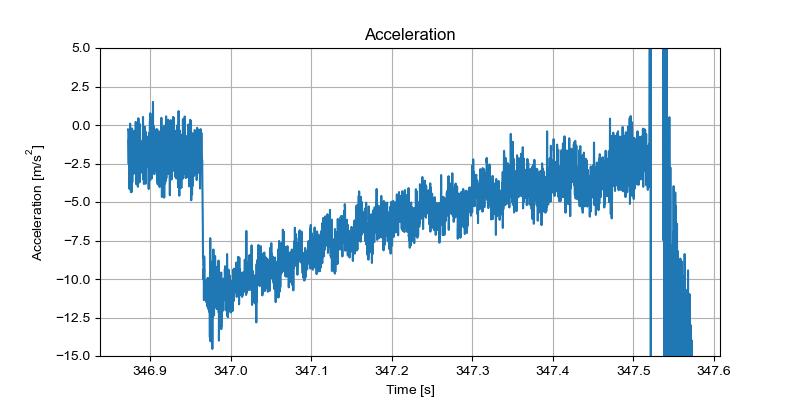
\includegraphics[width=0.9\linewidth]{pics/speedcalc.png}
    \caption{Acceleration during free fall used to calculate real drop speed}
    \label{fig:speedcalc}
\end{figure}

\begin{equation}
    \hat{v}_{calc} = \sqrt{2 * g * h}
    \label{equ:vcalc}
\end{equation}

The equations is derived by comparing the definitions of potential and kinetic energy as displayed in \autoref{equ:vcalcDer}. 

\begin{subequations}
    \begin{align}
    E_{pot} &= m * g * h \label{equ:Epot}\\
    E_{kin} &=  \frac{m * \hat{v}_{calc}^2 }{2} \\
    m * g * h &= \frac{m * \hat{v}_{calc}^2 }{2} \\
    \hat{v}_{calc} &= \sqrt{2 * g * h}
    \end{align}
    \label{equ:vcalcDer}
\end{subequations}


The indirectly measured peak velocity was calculated using \autoref{equ:vmes}.  The result was \( \hat{v}_{me} = 5,39 m/s \).

\begin{equation}
 \hat{v}_{mes} = g * t
 \label{equ:vmes}
\end{equation}

The equation is derived by considering the definition of speed as displayed in \autoref{equ:vmesDer}.
\begin{subequations}
    \begin{align}
    a &= g \\
    \hat{v}_{mes} &= \int a * dt \\
    \hat{v}_{mes} &= g * t
    \end{align}
    \label{equ:vmesDer}
\end{subequations}

The margin of error therefore was 0,55 \%. Considering the low margin of error, implementing a direct way to measure the impact speed is definitely recommendable but not of a high priority.

\section{Sample Types}

There are two types of samples which can be tested by the test rig. 

\begin{itemize}
    \item round specimen, with a diameter of 0,8 m
    \item square specimen, with an edge length of 1,5 m
\end{itemize}

The samples tested so far were all round. The test set up and sensor array are slightly different for the two test campaigns run so far. 

\subsection{Round Specimen}

The test is based on the test setup described by \textcite{c1550}, which has been widely used at Kiirunavaara Mine, for example \textcite{Thyni14} or \textcite{Erik15}. Please note that the test setup described by \textcite{c1550} is quasi-static. It was modified slightly to be a dynamic test. With the current setup it is not possible to conduct quasi-static tests. 

\begin{figure}
    \centering
    \subcaptionbox{Before the impact\label{fig:before}}
    {
    \begin{tikzpicture}
%pivot

\draw
(0,0) circle [radius = 0.5]
(-0.5,0) -- (-1,0) -- (-1,1) -- (1,1) -- (1,0) -- (0.5,0)
(3,1) -- (-1,1) -- (-1,3) -- (3,3);
\draw (-60:0.5) coordinate (start1)
(-120:0.5) coordinate (start2)
(-60:1) coordinate (end1)
(-120:1) coordinate (end2)
(start1) -- (end1) -- (end2) -- (start2);

\draw (-1,2) [left] node {sample}
(-1,0.5) [left] node {pivot};
(-1,-0.5) [left] node {load cell};
\end{tikzpicture}
    }
    \subcaptionbox{After the impact\label{fig:after}}
    {
    \begin{tikzpicture}[rotate=-10]
%pivot rotated

\draw
(0,0) circle [radius = 0.5]
(-0.5,0) -- (-1,0) -- (-1,1) -- (1,1) -- (1,0) -- (0.5,0)
(3,1) -- (-1,1) -- (-1,3) -- (3,3);

\draw (-50:0.5) coordinate (start1)
(-110:0.5) coordinate (start2)
(-50:1) coordinate (end1)
(-110:1) coordinate (end2)
(start1) -- (end1) -- (end2) -- (start2);

\draw (-1,2) [left] node {sample}
(-1,0.5) [left] node {pivot};
(-1,-0.5) [left] node {load cell};
\end{tikzpicture}
    }
    \caption{Effect of using a pivot instead of a stiff connection}
    \label{fig:pivot}
\end{figure}

\begin{figure}[p]
    \centering
    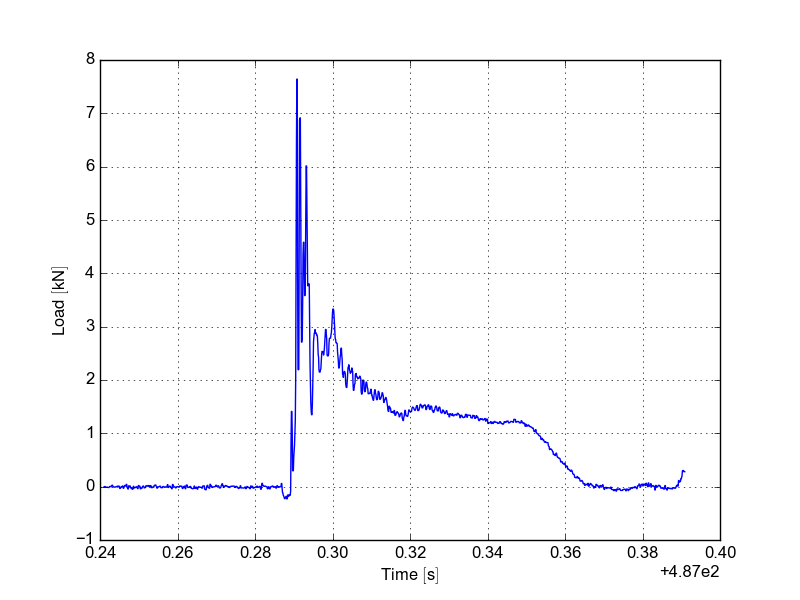
\includegraphics[width = 0.95 \linewidth]{pics/loadip.png}
    \caption{Dip in the force measurement of the load cells at the beginning of the impact}
    \label{fig:dip}
\end{figure}

\begin{figure}
    \centering
    \begin{tikzpicture}
%round sample

%text
\path (90:5) ++ (4,4) coordinate (start)
(-30:5) ++ (4,4) coordinate (end);
\draw [{Latex[length=3mm, width=1mm]}-{Latex[length=3mm, width=1mm]}] (start) arc (90:-30:5)
node [above, sloped,midway] {120\textdegree};


%sample
\draw(4,4) circle [radius=4];

%load cells
\draw (90:3.5) ++ (4,4) circle [radius=.5];
\draw (210:3.5) ++ (4,4) circle [radius=.5];
\draw (-30:3.5) ++ (4,4) circle [radius=.5];

%measurements
\draw[{Latex[length=3mm, width=1mm]}-{Latex[length=3mm, width=1mm]}]
(0,-1) -- (8,-1) node [above,midway] {0,8 m};

%text
\draw (210:5) ++ (4,4) node (load) {load cell}
(4,5) node {impact zone};

%impact zone
\path[clip] (4,4) circle [radius=0.5];
\foreach \x in {2.4,2.6,...,4.6}
\draw[ultra thin] (\x,3.3) -- ++ (2,2);

\end{tikzpicture}
    \caption{Top view of the test setup for the round sample}
    \label{fig:round}
\end{figure}

The specimen have a diameter of 0,8 m. They are placed on pivots on 3 load cells. See \autoref{fig:round}. The pivots enable the specimen to deform more freely as displayed in \autoref{fig:pivot}. In the second campaign the horizontal acceleration of the sample was recorded and found to be significant. Therefore some horizontal movement must occur.

For lighter samples with a thickness below 100 mm a slight dip in the measured load just before impact is recorded. See \autoref{fig:dip}. Probably the sample deforms and reduces the load on the load cells before the impulse is transferred to the load cells. This dip gets less pronounced as the thickness of the samples increases. 
The impact weight is dropped onto the center of the sample. The samples that were tested so far had a thickness of 50, 70 and 100 mm. Only fibre reinforced concrete was used. Unlike suggested by \textcite{c1550} the samples were not sprayed but cast, therefore no accelerators were used in the recipe. The samples were tested by dropping a weight on them once an recording the amount of damage.

\subsection{Square Specimen}
\begin{figure}
    \centering
    \begin{tikzpicture}
%3D square sample


%steel frame
\draw (0,12) rectangle ++(8,-0.3);
\draw (3.8,15.5) -- ++ (6,0)
(3.8,15.2) -- ++ (5.75,0)
(3.8,15.5) -- ++ (0,-0.3)
(3.8,15.2) -- ++ (-2.1,-2.7)
(8,11.7) -- ++ (3.2,4) -- ++ (0,0.3);
\begin{scope}
\pgftransformcm{1}{0}{0.4}{0.5}{\pgfpoint{0}{12cm}}
\draw (0,0) rectangle (8,8);
\draw (1,1) rectangle (7,7);
\end{scope}



%mesh
\begin{scope}
\pgftransformcm{1}{0}{0.4}{0.5}{\pgfpoint{0}{-4.5cm}}
\draw [step=1] (0,0) grid (8,8);
\end{scope}

%concrete slab
\begin{scope}
\pgftransformcm{1}{0}{0.4}{0.5}{\pgfpoint{0}{7cm}}
\draw[fill=lightgray] (0,0) rectangle (8,8);
\draw[fill=black] 
(1.5,1.5) circle [radius = 0.1]
(6.5,1.5) circle [radius = 0.1]
(1.5,6.5) circle [radius = 0.1]
(6.5,6.5) circle [radius = 0.1]; 
\end{scope}
\draw[fill=lightgray] (0,7) rectangle (8,5);
\begin{scope}
\pgftransformcm{0}{1}{0.4}{0.5}{\pgfpoint{8cm}{7cm}}
\draw[fill=lightgray] (0,0) rectangle (-2,8);
\end{scope}
\begin{scope}
\pgftransformcm{1}{0}{0.4}{0.5}{\pgfpoint{4cm}{7cm}}
\draw[fill=white] (0,4) circle [radius = 2];
\end{scope}


%sample
%\draw[fill=gray] 
(0.2,0.25) rectangle ++ (0.5,0.5)
(7.7,0.25) rectangle ++ (0.5,0.5)
(0.5,0) rectangle (7.5,0.5);
\draw[fill=gray]
(0.7,0.25) rectangle (7.7,0.75);

    %side
\begin{scope}
\pgftransformcm{0}{1}{0.4}{0.5}{\pgfpoint{7.5cm}{0cm}}
\draw[fill=gray] (0,0.5) rectangle ++ (0.5,7);
\end{scope}

    %top
\begin{scope}
\pgftransformcm{1}{0}{0.4}{0.5}{\pgfpoint{0}{0.5cm}}
\draw[fill=gray]
(0.5,0.5) -- (7.5,0.5) -- (7.5,7.5) -- (0.5,7.5) --  cycle;
    %bolt
\draw[fill=black] 
(1.5,1.5) circle [radius = 0.1]
(6.5,1.5) circle [radius = 0.1]
(1.5,6.5) circle [radius = 0.1]
(6.5,6.5) circle [radius = 0.1]; 
\end{scope}

%bolts
\draw[ultra thin] 
(2.1,9.5) -- ++ (0,-15) coordinate [pos=0.95] (bolt1)
(7.1,9.5) -- ++ (0,-15) coordinate [pos=0.95] (bolt2)
(4.1,11.5) -- ++ (0,-15) coordinate [pos=0.95] (bolt3)
(9.1,11.5) -- ++ (0,-15) coordinate [pos=0.95] (bolt4);

%Text
\draw
(12,14) node [right,align =left] {steel frame}
(12,7) node [right,align =left] {concrete slab}
(12,2) node [right, align = left] {sample}
(12,-3) node [right,align = left] {mesh}

(5,-6) node (bolts) {bolts};
\draw[-{Latex[length=3mm, width=1mm]}]
(bolts) -- (bolt1);
\draw[-{Latex[length=3mm, width=1mm]}]
(bolts) --(bolt2);
\draw[-{Latex[length=3mm, width=1mm]}]
(bolts) -- (bolt3);
\draw[-{Latex[length=3mm, width=1mm]}]
(bolts) -- (bolt4);

\end{tikzpicture}
    \caption{Sketch of the sample setup for the large scale tests}
    \label{fig:SAMPLE}
\end{figure}


\begin{figure}
    \centering
    
    \subcaptionbox{Top view of concrete slab}{
    \begin{tikzpicture}
%size concrete slab

%concrete slab
\draw (0,0) rectangle (9,9)
(4.5,4.5) circle [radius = 2.1]
(1.5,1.5) circle [radius = 0.1]
(7.5,1.5) circle [radius = 0.1]
(1.5,7.5) circle [radius = 0.1]
(7.5,7.5) circle [radius = 0.1];


\path (225:2.1) -- ++((4.5,4.5) coordinate [at end] (end);

%measurements
\draw [{Latex[length=3mm, width=1mm]}-{Latex[length=3mm, width=1mm]}] 
(0,-1) -- (1.5,-1)
node [midway, above] {0,25 m};
\draw [{Latex[length=3mm, width=1mm]}-{Latex[length=3mm, width=1mm]}] 
(7.5,-1) -- (9,-1)
node [midway, above] {0,25 m};
\draw [{Latex[length=3mm, width=1mm]}-{Latex[length=3mm, width=1mm]}] 
(1.5,-1) -- (7.5,-1)
node [midway, above] {1,0 m};
\draw [{Latex[length=3mm, width=1mm]}-{Latex[length=3mm, width=1mm]}] 
(0,-2) -- (9,-2)
node [midway, above] {1,5 m};

%cut
\draw [dashed]
(0,4.5) -- (4.5,4.5)
node [near start,above] {profile A}
(4.5,1.5) -- (9,1.5)
node [midway,above] {profile B};


\draw [{Latex[length=3mm, width=1mm]}-{Latex[length=3mm, width=1mm]}] 
(10,0) -- (10,1.5)
node [midway, above, sloped] {0,25 m};
\draw [{Latex[length=3mm, width=1mm]}-{Latex[length=3mm, width=1mm]}] 
(10,7.5) -- (10,9)
node [midway, above, sloped] {0,25 m};
\draw [{Latex[length=3mm, width=1mm]}-{Latex[length=3mm, width=1mm]}] 
(10,1.5) -- (10,7.5)
node [midway, above, sloped] {1,0 m};
\draw [{Latex[length=3mm, width=1mm]}-{Latex[length=3mm, width=1mm]}] 
(11,0) -- (11,9)
node [midway, above, sloped] {1,5 m};

%radius
\draw [{Latex[length=3mm, width=1mm]}-]
(end) -- ++ (1.45,1.45);
\path 
(end) -- ++ (2.15, 2.15)  node [pos=1, sloped, above] {R = 0,35 m};



\end{tikzpicture}
    }
    \subcaptionbox{Side view of concrete slab}{
    \begin{tikzpicture}
%side view concrete slab

%text
\draw
(2.25,3.5) node {profile A} 
(6.75,3.5) node {profile B}; 


%measurements
\draw [{Latex[length=3mm, width=1mm]}-{Latex[length=3mm, width=1mm]}] 
(0,-1) -- (2.4,-1)
node [midway, above] {0,4 m};
\draw [{Latex[length=3mm, width=1mm]}-{Latex[length=3mm, width=1mm]}] 
(4.5,-1) -- (2.4,-1)
node [midway, above] {0,35 m};
\draw [{Latex[length=3mm, width=1mm]}-{Latex[length=3mm, width=1mm]}] 
(4.5,-1) -- (7.5,-1)
node [midway, above] {0,5 m};
\draw [{Latex[length=3mm, width=1mm]}-{Latex[length=3mm, width=1mm]}] 
(9,-1) -- (7.5,-1)
node [midway, above] {0,25 m};
\draw [{Latex[length=3mm, width=1mm]}-{Latex[length=3mm, width=1mm]}] 
(0,-2) -- (9,-2)
node [midway, above] {1,5 m};
\draw [{Latex[length=3mm, width=1mm]}-{Latex[length=3mm, width=1mm]}] 
(10,0) -- (10,2.4)
node [midway, above, sloped] {0,4 m};


%left rect
\draw (2.4,0) -- (4.5,0)
(2.4,2.4)-- (4.5,2.4);

%cutLine
\draw[dashed] (4.5, 4) -- ++ (0,-5);

\draw[fill = lightgray] (0,0) rectangle (2.4,2.4)
(4.5,0) -- (9,0) -- (9,2.4) -- (4.5,2.4);

%bolt
\draw [thick] (7.5,0) -- (7.5,2.4)
node [at end, above] {bolt};

\end{tikzpicture}
    }

\caption{Views and dimensions of the concrete slab}
\label{fig:con}
\end{figure}

\begin{figure}
    \centering
    \begin{tikzpicture}
%sample size

%sample
\draw
(0,0) -- (7.8,0) -- (7.8,7.8) -- (0,7.8) -- cycle;

%bolts
\draw 
(0.9,0.9) circle [radius = 0.1]
(0.9,6.9) circle [radius = 0.1]
(6.9,6.9) circle [radius = 0.1]
(6.9,0.9) circle [radius = 0.1];

%measurements
\draw [{Latex[length=3mm, width=1mm]}-{Latex[length=3mm, width=1mm]}]
(0,-1) -- (0.9,-1) node [midway, above] {0,15 m};
\draw [{Latex[length=3mm, width=1mm]}-{Latex[length=3mm, width=1mm]}]
(0.9,-1) -- (6.9,-1) node [midway, above] {1,0 m} ;
\draw [{Latex[length=3mm, width=1mm]}-{Latex[length=3mm, width=1mm]}]
(6.9,-1)--(7.8,-1) node [midway, above] {0,15 m};

\draw [{Latex[length=3mm, width=1mm]}-{Latex[length=3mm, width=1mm]}]
(0,-2) -- (7.8,-2) node [midway, above] {1,3 m} ;


\draw [{Latex[length=3mm, width=1mm]}-{Latex[length=3mm, width=1mm]}]
(8.8,0) -- (8.8,0.9) node [midway, above, sloped] {0,15 m};
\draw [{Latex[length=3mm, width=1mm]}-{Latex[length=3mm, width=1mm]}]
(8.8,0.9) -- (8.8,6.9) node [midway, above, sloped] {1,0 m} ;
\draw [{Latex[length=3mm, width=1mm]}-{Latex[length=3mm, width=1mm]}]
(8.8,6.9)--(8.8,7.8) node [midway, above, sloped] {0,15 m};

\draw [{Latex[length=3mm, width=1mm]}-{Latex[length=3mm, width=1mm]}]
(9.8,0) -- (9.8,7.8) node [midway, above, sloped] {1,3 m} ;
\end{tikzpicture}
    \caption{Top view and dimensions of the specimen}
    \label{fig:spes}
\end{figure}

This test setup was suggested by \textcite{Erik15}. In \autoref{fig:SAMPLE} a 3d sketch of the setup is displayed, please note that it is not to scale and merely serves to illustrate the basic principle. and in \autoref{fig:con} and \autoref{fig:spes} the dimension of the concrete slab and the specimen are given. %Please note that the specimen thickness was one of the variables that was varied in the course of the tests. It ranged between 50 and 100 mm.

The steel frame is only roughly sketched. It serves to attach the mesh to the sample and pretension it. It is bolted into the concrete slab. In \autoref{fig:frame} a picture of the frame already bolted into the sample is given.

\begin{figure}
    \centering
    \includegraphics[width = 0.95\linewidth]{pics/steelframe.jpg}
    \caption{Steel frame mounted on sample}
    \label{fig:frame}
\end{figure}

The concrete slab has several functions. First it simulates the static load resting on the surface support, second as the sample is cast directly on it, the adhesion between rock and shotcrete is simulated. The concrete slab has a round opening in the center with a diameter of 70 cm. This marks the impact zone of the drop weight.  

Both sample and slab are cast from the same concrete, C50, which means it has a uniaxial compressive strength of approximately 50 MPa after 28 days. If fibres are used the fibre content of the concrete is \(40 ~\frac{\text{kg}}{\text{m}^3}\). The sample productions is a two step process. First a concrete slab is cast, which then cures for 28 days, afterwards the sample is cast on top and again cures for 28 days. Afterwards the sample is ready to be tested. 

The adhesive forces between sample and concrete slab are meant to simulate the adhesive forces between shotcrete and rock. Cast concrete is quite smooth but the rock mass surface is quite rough. That is why the surface of the concrete slab has to be roughened before casting the sample. Please also note that the specimen is cast on instead of sprayed on, as it would be \textit{in - situ}. 

The test panel will be attached to the concrete slab with 4 bolts as well. These bolts are simulated by threaded M30 bars, with the previously discussed plates and nuts. The nuts are applied using a torque wrench to keep the applied force consistent. % TO DO description of the bolts and preload force
The intend is to simulate \textit{in - situ} conditions as closely as possible. As well as keep the specimen from simply dropping to the ground after the the adhesive bond breaks. The concrete slab rests on 4 load cells located at the corners. The specimen should only be supported by the bolts and therefore can not have the same outline as the concrete. That is why the edges have to be removed .% and the sample has a cloverleaf shape. If these inward turned corners have any effect on the testing or if they form weak points remains to be seen.
It was also considered to simply remove the corners from the sample, creating a cloverleaf shape. This would have yielded more surface area for the sample. If the resulting inward turned corners have any effect on the testing is not clear.

%The testing method is of yet not defined. For this thesis 2 samples of each type are planned. The current idea would be to start at 1 kJ and increase the load by one kJ with every hit, measure the destruction and see how long the sample survives. This would test both the fatigue resistance and provide a conservative estimate about the maximum survivable impact energy. But this is still being discussed and not decided yet.

\begin{figure}
    \centering
    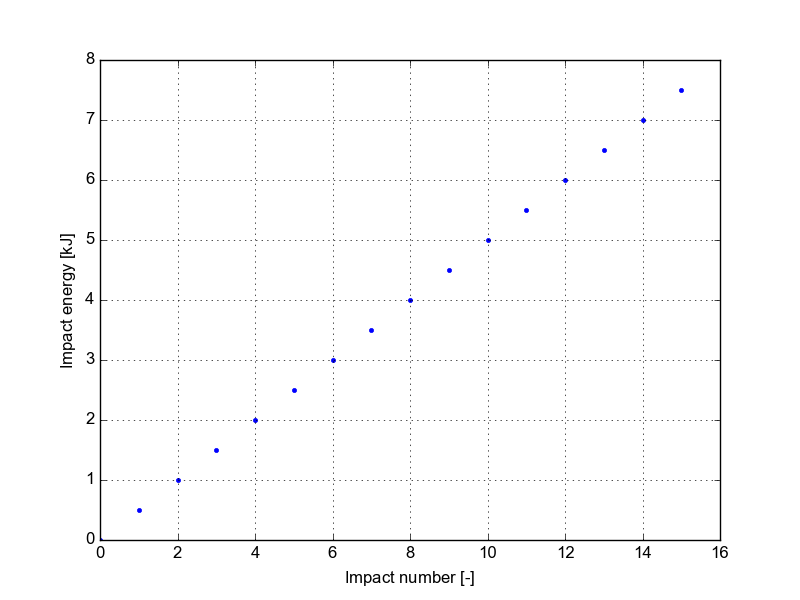
\includegraphics[width = 0.95\linewidth]{pics/impact_energy.png}
    \caption{Energy of each individual impact}
    \label{fig:impactenergy}
\end{figure}

\begin{figure}
    \centering
    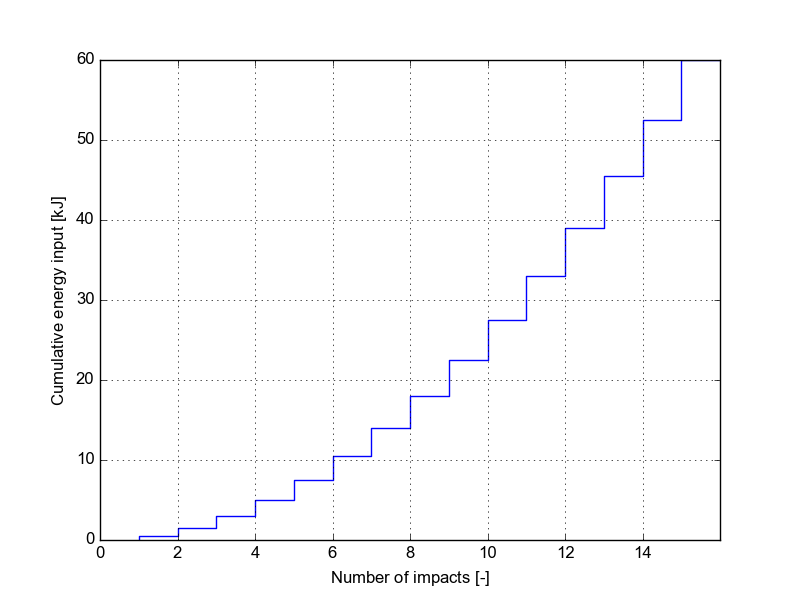
\includegraphics[width = 0.95\linewidth]{pics/cum_energy.png}
    \caption{Total energy}
    \label{fig:cumenergy}
\end{figure}

The testing method is a combination of both categories discussed in \autoref{sec:droptest}. Two samples of a given type are necessary. The first sample will be loaded in multiple impacts. The first impact will have 0,5 kJ and the following impacts will increase by 0,5 kJ.  See \autoref{fig:impactenergy}. The sample probably can with stand an almost endless number of very low energy impacts. Like a concrete wall cannot be destroyed by throwing a tennis ball at it. To keep this from happening the energy of the impacts increases with every hit.
The cumulative energy increases rapidly using this method. See \autoref{fig:cumenergy}.
As the drop weight has a very strong influence on the results of the test, only the 1000 kg drop weight will be used.

This test has two functions. Firstly to show much cumulative energy a sample can survive and secondly to show how the sample handles repeat impacts.

The second sample will be hit by a single impact. This impact will have 50 \% of the cumulative energy the first sample survived. This test will yield information about the largest single impact a sample can survive.

\begin{figure}
    \centering
    \begin{tikzpicture}
%size mesh

%boundary
\path [draw] (0,0) rectangle (4.4,4.6);

%mesh
\draw [help lines, step = .1] (0,0) grid (4.4,4.6);

%bolts
\draw [fill = gray] 
(0.1,0.15) circle [radius= 0.05]
(0.1,2.3) circle [radius= 0.05]
(0.1,4.45) circle [radius= 0.05]

(2.2,.15) circle [radius= 0.05]
(2.2,2.3) circle [radius= 0.05]
(2.2,4.45) circle [radius= 0.05]

(4.3,.15) circle [radius= 0.05]
(4.3,2.3) circle [radius= 0.05]
(4.3,4.45) circle [radius= 0.05];

%measurements
\draw [{Latex[length=3mm, width=1mm]}-{Latex[length=3mm, width=1mm]}] 
(0,-1) -- (4.4,-1)
node [midway, above] {2,2 m};
\draw [{Latex[length=3mm, width=1mm]}-{Latex[length=3mm, width=1mm]}] 
(5.4,0) -- (5.4,4.6)
node[midway, sloped, above] {2,3 m};
\draw[red, dashed, thick]
(-0.2,2.3) -- (2.2,2.3) -- (2.2,-0.2);

\end{tikzpicture}
    \caption{\textit{In-situ} boundary conditions of mesh}
    \label{fig:insituMesh}
\end{figure}

For testing of mesh the boundary conditions are very important. \autocite[5]{villa09} This is especially true for the square sample tests as these try to be as realistic as possible.
The welded mesh currently in use is applied in panels with a size of 2,3 on 2,2 m and a bolt spacing of 1 bolts per meter. See \autoref{fig:insituMesh}. Which means that a 1 x 1 m square of mesh has two open boundaries and two flexible boundaries (illustrated in \autoref{fig:insituMesh} with red dashed lines). Which means that during testing two ends of the mesh should be free and two should be constrained. 
Chain-link and textile mesh can be applied in much larger continuous pieces. Therefore all their boundaries should be confined.

%Therefore this modification to the test rig will allow to vary boundary conditions of the mesh between very stiff and open and even allow pretensioning as needed. The basic principle would be to pull up and attach the mesh to the sides of a concrete slab. %Possible ways of attachment would be addition bolts for example. 
%The drawbacks of this method lie in the very difficult sample preparation, firstly the corners would need to be cut from each sample to give it a clover leaf shape. %as displayed in \autoref{fig:meshBound}. 
%The leaves would need to be bent at a 90 degree angle. This is a lot of preparatory work necessary for a single test. %Ideally the lacing would be attached as one continuous rope and be allowed to glide 

\section{Impact Cushion}

The test weights are made of steel and have sharp edges. During a  seismic impact the accelerated rocks do not strike the surface support directly but first hit a zone of loose and broken rock that forms around the circumference of the excavation which distributes the load across a larger area and cushions the impact slightly. In order to simulate realistic conditions a rubber cushion will be put between drop weight and test panel to distribute the load more evenly. Gravel was also considered as a possible cushion, which would have been even closer to reality and is commonly used in similar tests. The drawback of gravel would be that the energy dissipated through crushing is not known and could vary between experiments, while the deformation energy of a rubber plate should be fairly consistent and calculable.

%As described in the literature review, most cushions used up until now were made from bricks or gravel. For the large scale tests test rubber mats will be used. Rubber mats have to advantage that they have very exactly defined properties. See \autoref{tab:cushion}

\begin{table} [h]
    \centering
    \begin{tabular}{ll}
    \toprule
    Property & typical value \\
    \midrule
    Hardness     &  60  \textdegree IRHD\\
    Density & 1,13 \( \frac{\text{g}}{\text{cm}^3} \) \\
    Tensile strength & 19,5 MPa \\
    Elongation at break & 510 \% \\
    \bottomrule
    \end{tabular}
    \caption{Properties of the rubber cushion after \autocite[76]{metso18}}
    \label{tab:cushion}
\end{table}

The exact material used in this test was Metso Trellex T60. See \autoref{tab:cushion}. Two circles with a diameter of approximately 70 cm and a thickness of 25 mm were glued together to form an impact cushion. 
%TO DO take a nice picture

%As material parameters are already defined and guaranteed by the producer.

\section{Shape of Drop Weight}

As the drop weights have large cutouts on either side for the guide rails, air should be able to escape upward without forming a cushion and slowing the final descend of the weight. These cutouts have the drawback that modelling the drop weight is not a trivial task. A numerical analysis of the drop tests is outside of the scope of this thesis. If a numerical model would be required, the shape of the drop weights would probably have to be changed and channels for air to escape from the impact site would have to be created. Or other steps would have to be taken to make the cross section of the weights more suitable for modelling. 
%TO DO picture or drawing of the drop weight

\section{Sensors}

The main objective of the sensor array is to have at least 100 measurements during the critical part of the experiment. Which means that the first peak of each parameter could be characterized by 100 measurements. Especially load and displacement need to be measured with utmost care. Load displacement curves are the best way to calculate the absorbed energy. \autocite[5]{player04} 
In \autoref{tab:senrequl} the critical times for each parameter and the therefore necessary minimal resolution are given.

\begin{table}[h]
    \centering
    \begin{tabular}{lrr}
    \toprule
         Parameter & Critical time [ms] & Required resolution \\
    \midrule
         Force & 20 & 5 kHz\\
         Displacement & 50 & 2 kHz \\
         Acceleration of drop weight & 20 & 5 kHz \\
         Velocity &  20 & 5 kHz \\
    \bottomrule
    \end{tabular}
    \caption{Required sensor resolutions}
    \label{tab:senrequl}
\end{table}

Therefore the following sensor array was chosen, as displayed in \autoref{tab:senarrl}. According to the suggestion made by \textcite{Erik15} and to have reliable measurements if one of the sensors should malfunction important parameters were measured redundantly. Especially the accelerometer measurements are very versatile. Velocity can be calculated by integrating the measured acceleration over time. Displacement can be calculated by numerically integrating the acceleration over time twice. This was attempted but the results suffered both zero off-set and zero drift. This why they were not included in the analysis. According to \textcite[3]{ansell02} this is both usual and expected.
The force applied by the drop weight can be calculated quite easily: \(F = m * a\). %Of course there is a difference between the force measured by the accelerometer and the load cells, as it is measured in different places.

\begin{table}[h]
    \centering
    \begin{tabular}{lll}
    \toprule
         Parameter & Primary Sensor & Secondary Sensor  \\
    \midrule
         Velocity &  (Accelerometer) & \\
         Force & Load cells & Accelerometer \\
         Displacement & Laser sensor & High speed camera \\
         Acceleration of Drop weight & Accelerometer & \\
         Drop height & Rotary encoder & \\
    \bottomrule
    \end{tabular}
    \caption{Required sensor array}
    \label{tab:senarrl}
\end{table}

\begin{table}
    \centering
    \begin{tabular}{ll}
    \toprule
    Sensor & Type \\
    \midrule
Loadcell & HBM C6A \\
& HBM U10M\\
Laser sensor & SICK 0D1000\\
Accelerometer & Kistler 8704B5000  \\
& PCB 305B03\\
High speed camera & Casio Exilim Pro Ex-F1 \\
& Phantom Miro LC110 \\
Rotary encoder & Leine Linde RHI 503 \\

\bottomrule
    \end{tabular}
    \caption{Overview of the deployed sensors}
    \label{tab:senover}
\end{table}

The sensors chosen for each specific task are listed in \autoref{tab:senover}. %Their technical data sheets are in the Appendix.

The exact sensor array for each test series varies slightly, as it iterated towards the finalized version. The sensor array used in each campaign is described in \autoref{cha:res}. 

As a few sensors were added on later, several Data Logging systems were used which had to be synchronised manually in the post-processing.
The main data logging was done using a HBM MX879B. As main amplifier a HBM MX840B was used. The additional accelerometers were logged using a MREL Data Trap II\textsuperscript{TM}. The signal was amplified using a PCB 480B21. The high speed camera footage was logged by the internal memory of the camera and a standard SD card. 

\subsection{Load Cells}

The load cells are located at the edge of the sample and measure the force of the impact. The difference between the potential energy of the drop weight and this measured is the deformation energy absorbed by the test panel as well as any other kinds of dissipated energy through for example heat or vibrations.

For the round samples, 3 loadcells are used. See \autoref{fig:round}. The sample rests on pivots on top of the load cells. The load cells have a maximum load of 250 kN each. The sampling rate is 10 kHz. 

For the square sample 4 load cells are used. The concrete slab rests on the load cells. The force of the impact by the drop weight travels through the sample and then either directly the through the adhesive contact or the threaded bar bolts into the concrete block and then into the load cells. The load cells have a maximum capacity of 1 MN each.

\subsection{Laser Sensor}
\label{ssec:laser}

The largest displacement was expected at the center of the sample. To not disturb the measurement a non-contact sensor was chosen, a laser distance sensor. 
It is located underneath the sample. As some samples break and pieces could damage the sensor, it has to be protected. That is why it is placed horizontally, slightly away from the center and underneath steel plating and the laser beam reflected by a mirror to hit the center of the sample.

\subsection{Accelerometers}

The test site is underground and humid. Therefore sensors have to be robust. Piezoresistive sensors would give better results, especially when integrating for velocity and displacement, but are more sensitve. Piezoelectric accelerometers can not measure gravity or other constant accelerations, because the piezoelectric sensor element only produces electricity when it experiences a change in acceleration. %Therefore they can only measure changes in acceleration. 
They also have signal decay, which means that the output of the sensor does not immediately drop to zero when the acceleration does. But for the short impacts and high frequencies expected from the drop tests they should be good enough. \autocite{Hanly16} %Especially since they are only secondary sensors.  

Two types of accelerometers were used. 
Both of them are piezoelectric and uniaxial. 
The PCB sensors are more sensitive with \(0,05~\frac{\text{mV}}{(\text{m/s}^2)}\) output and \(\pm 98.000~\frac{\text{m}}{\text{s}^2}\) measuring range.
The Kistler sensors have an output of \(0,1~\frac{\text{mV}}{(\text{m/s}^2)}\) and \(\pm 49.000~\frac{\text{m}}{\text{s}^2}\) measuring range. 
That is why the PCB sensors will be used in positions with higher priority. Except for the drop weight. 
As the thread for a Kistler accelerometer is drilled directly into the weight itself it is impossible to use PCB acceleromters in this position without an adapter.

There are several ways to mount accelerometers. For example using magnets, adhesive or studs. As studs have the best frequency response this mounting method was used primarily. \autocite[24]{Hanly16} The accelerometers on the drop weight were mounted directly. For the other applications steel plates measuring 5 x 5 x 0.8 cm with a hole at the center were manufactured. They were glued in place and the accelerometers were screwed into the central hole.  A slight problem was that the Kistler and PCB accelerometers had different threads, M6 and 1/4" respectively. Using a uniform system would streamline the setup of tests. Exchanging the accelerometers could be considered in future applications.

The drop weight is fitted with an accelerometer that is logged by the main system. In later tests more accelerometers were added. Their respective positions and mounting will be discussed in detail in the description of the set up of each test.

\subsection{Drop Height}

The drop height together with the drop weight is the defining parameter of the kinetic energy available. It is measured by a rotary incremental encoder with a resolution of 500 pulses per revolution. As the testing procedure requires the drop weight to be lowered until it is almost touching the sample. This is done so the measurements of the rotary encoder are reset. The drop height is then calculated from difference between the distance the drop weight is lifted up and the distance it is lowered down. The drop weight is not supposed to touch the sample when it is at the lowest point. This was tested by running a sheet of paper between sample and drop weight.
Due to this constraint imposed by the testing procedure the accuracy of the drop height measurements is significantly lowered compared to the accuracy of the rotary encoder. The accuracy of the drop height measurements is assumed to be $\pm~0,5$ mm. 

\subsection{Drop Weights}

There currently are 5 drop weights available: 50 kg, 100 kg, 200 kg, 500 kg, 1000 kg. The two smallest weights have been modified, their bottom is not flat but optimised to provided a point load.

%TO DO, input a picture of the smaller drop weights
%TO DO, make a sketch of the drop weights

%"Sensor frequency must fit with impact time" Nikolaos Petropoulos in conversation. If you want to measure something that takes almost no time at all, you better have a fucking high measuring frequency! 

\subsection{High Speed Camera}

%TO DO enhance this ugly as fuck graphic!
\begin{figure}
    \centering
    \begin{tikzpicture}
%HORRIBLE camera picture

%displacement
%\draw (1,2.5) parabola bend (3.25,2) (5.5,2.5) node [midway] (down) {this};

%camera
\draw (0,0) -- ++ (0,1.95);
\draw [fill = black]
(-0.25,1.95) rectangle ++ (.5,.5)
(0.25,2.35) -- ++ (0.2,0.1) -- ++ (0,-0.3) -- ++ (-0.2,0.1);

%\draw[ultra thin] (0.25,2.2) -- (5.6,2.4)
%(0.25,2.2) -- (5.6,2);

%sample
\draw
(1,2.5) rectangle ++ (4.5,1.5); 

%ruler
\draw 
(5.6,0) -- (5.6,3.2) -- (5.8,3.2) -- (5.8,0) ;
\foreach \x in {0,0.8, ..., 3.2}
\draw [fill = black]
(5.6,\x) rectangle ++ (0.2,0.4);

%central line
%\draw[ultra thin,dashed] (3.25,4) -- (3.25,0);

%distances
%\draw [{Latex[length=3mm, width=1mm]}-{Latex[length=3mm, width=1mm]}] 
%(0,-1) -- (3.25,-1) node [midway, above] {1,0 m};
%\draw [{Latex[length=3mm, width=1mm]}-{Latex[length=3mm, width=1mm]}] 
%(3.25,-1) -- (5.5,-1) node [midway, above] {0,75 m};
%\draw [{Latex[length=3mm, width=1mm]}-{Latex[length=3mm, width=1mm]}] 
%(0,-2) -- (5.5,-2) node [midway, above] {1,75 m};

%text
\draw (0,3) node {camera}
(3.25,4.5) node {sample}
(5.5,1) node [left] {ruler};

%\draw [{Latex[length=3mm, width=1mm]}-{Latex[length=3mm, width=1mm]}] (3.25,2.5) -- (down);

\end{tikzpicture}
    \caption{Camera set up}
    \label{fig:cam}
\end{figure}

 A Casio Exilim Pro Ex-F1 did all the filming of the tests run for this thesis, it has a maximum frame rate of 1200 frames per second (fps) and a resolution of 336 x 96 Pixel at that setting. At 600 fps the resolution is 432 x 192 Pixel.
As stated in \autoref{tab:senrequl} the minimal resolution for displacement measurement would be 2 kHz. The camera only has 0,8 kHz at its highest setting. Which makes the camera unsuitable as a primary measurement device without compromising the precision goals. But it is useful a secondary sensor, for qualitative assessment and as a confidence check for other sensors.
\begin{comment}
The camera is located approximately one meter away from the center of the sample, where the highest deformations are expected and the rulers are located on the other side of the sample, so about 1,75 m away from the camera. As displayed in \autoref{fig:cam}.


\begin{align*}
\frac{x}{1,0 m} &= \frac{0,01 m}{1,75 m}\\[5pt]
x &= \frac{0,01 m * 1,0 m}{1,75 m} \\
x &= 0,005714 m = 6 mm 
\end{align*}
\label{equ:def}


A quick calculation reveals that the 1 cm deflection measured on the ruler at a distance of 1,75 m is equal to approximately 6 mm of deformation at the center of the sample, 1,0 m away from the camera. As displayed in \autoref{equ:def}
As the expected deformations are quite small this value is assumed to be constant for all deformations. 

%At 1200 fps the 1 cm stripes of the ruler are represented by 3 to 4 pixels. Therefore measurements have an approximate error of \textpm 2 mm from the resolution of the camera alone. At a lower frame rate the error will go down but, but also will the measuring frequency.
\end{comment}

A small literature review revealed that in similar setups much more powerful cameras were used. For example \textcite{Kukolj2018} used a set up with 24,656 fps at 336 x 336 pixels, the application was tracking the propagation of cracks. %A frame rate exceeding 10.000 fps would be sufficient, for the estimated impact time of 20 ms, 200 frames would be available. The camera is located approximately one meter away from the point of expected maximum deformation.

Therefore a stronger high speed camera was sourced. A Phantom Miro LC110. This high speed camera is very sensitive and a safety cage was constructed from polycarbonate sheet and wood to protect it against possible impacts by pieces of a sample.%The resolution at different frame rates is displayed in \autoref{tab:LC110}.
%It was only used in one test and an operator mistake deleted the footage.

\begin{comment}
\begin{table}
    \centering
    \begin{tabular}{ll}
    \toprule
    Resolution & fps \\
    pixel x pixel & \\
    \midrule
    1280 x 720 & 1630 \\
    1280 x 720 & 1810 \\
    896 x 720 & 2520 \\
    640 x 480 & 5090 \\
    512 x 512 & 5790 \\
    384 x 288 & 12.900 \\
    256 x 256 & 19.800 \\
    128 x 128 & 60.400 \\
    128 x 64 & 113.200 \\
    128 x 8 & 400.000 \\
    64 x 8 & 400.000 \\
    \bottomrule
    \end{tabular}
    \caption{Possible resolutions of a Phantom Miro LC110}
    \label{tab:LC110}
\end{table}
\end{comment}

A high speed camera has a high shutter speed, which means that providing sufficient amounts of lights is crucial. Modern powerful lamps use mostly LED because it requires less power to produce the same amount of light when compared to other methods of producing light. 
But it is an inherent property of LED lights that they flicker when connected to an alternating current, for example when connected to the power grid \autocite[74]{steffen07} This flicker has a very high frequency and is not visible to the human eye. But it can distort the footage of high speed camera with a sufficiently high frame rate. Therefore alternative light sources might have to be used if the frame rate is very high. For the experiments conducted for this thesis LED lamps were sufficient. 

The very high amount of light disturbed the laser sensor readings.

Footage with 5000 fps and a resolution of 640 x 480 revealed strong bouncing of the sample which was only hinted at by the previous footage. This bouncing is far from the conditions encountered \textit{in - situ}. \textit{In - situ} the shotcrete is attached to rock and cannot dissipate energy through bouncing.   
%An array of 3 halogen lamps with a total of 26.250 lumen was used.

 




\chapter{Tests}
\label{cha:test}

 In order to be able to tell specimen apart quickly, the following naming convention was followed.

\section{Naming Convention}

A specimen name is assembled as follows:


\centering
\textbf{date\_description\_thickness[mm]\_energy level [kJ](\_repetition number)}
\flushleft

\subsection*{Date}

The international standard date notation is used. Year-Month-Day.

\subsection*{Description}

\begin{table}
\centering
\begin{tabular}{lr}
\toprule
Description & Shorthand \\
\midrule
plain shotcrete & s\\
fibre reinforced shotcrete & frs \\
welded mesh reinforced shotcrete & mrs \\
chain-link mesh reinforced shotcrete & crs \\
textile mesh reinforced shotcrete & crs \\
\hline
welded mesh underneath & + w \\
chain-link underneath & + c \\
textile mesh & + t\\
fjällband underneath & + j\\
lacing underneath & + l\\
TSL underneath & + s\\
\bottomrule
\end{tabular}
\caption{Sample description}
\label{tab:samdes}
\end{table}
%As of yet only round frs samples have been tested. So this section of the name starts with R to mark round samples and continues with frs to denote the composition. All current samples therefore have the same notation: Rfrs.

The description of the specimen is slightly more complicated, it was developed to be able to be used in future tests as well and is over complete. The first part is the test method:

\begin{itemize}
    \item dynamic tests are not marked (standard)
    \item \textbf{Q} marks quasi-static tests
    \item \textbf{C} marks samples that were tested quasi static after a dynamic test (combination)
\end{itemize}

The next part is the sample shape.

\begin{itemize}
    \item square samples are not marked (standard)
    \item \textbf{W} marks square samples without adhesion to the concrete slab
    \item \textbf{R} marks round samples
\end{itemize}

Lastly the composition of the panel, as described in \autoref{tab:samdes}. Please note that the composition is named starting from top to bottom. 


\subsection*{Energy Level}

The energy levels are given in kJ and are rounded to one decimal place and calculated using \(E_{pot} = m * g *h \), with \(g =9,8~\frac{\text{m}}{\text{s}^2}\). %Of course some of this calculated energy is dissipated, for example through vibrations of the rig and bouncing of the impact weight. The exact amount of energy absorbed by the specimen is therefore unknown.

This naming scheme fails for test that have been subjected to multiple impacts. for the tests both the total energy input and the impact are required. This can be achieved by writing XmY, with X denoting the energy of the impact and Y the total energy input into the panel.

\subsection*{Number of Repetitions}

The number of repetition is only used for the second and following repetitions. Therefore the first sample of a given composition is not marked especially. This makes it easier to spot tests with several repetitions.

\subsection*{Examples}

\centering
\textbf{19-06-21\_Qs+m+j+j\_150\_0\_3}
\flushleft

Would be a quasi-static test run on 2019-06-21 on a square specimen, made of plain shotcrete that has external mesh and two layers of Fjällband and is plain shotcrete. The specimen has a thickness of 150 mm, as the test is quasi-static the energy level is zero, and it is the third test run in this setup on that day.

\medskip
\centering
\textbf{18-12-04\_Rfrs\_50\_0,3}
\flushleft

Would be a test run on 2018-12-04 on a round specimen made from fibre reinforced concrete with a thickness of 50 mm, an energy level of 0,3 kJ and it would be the first test in this setup.


The tests were spaced out over a long time span and the sensor array changed several times during testing. In \autoref{tab:con} an overview of the different testing conditions is given. 


\begin{table}
    \centering
\begin{tabular}{l l l l l l l}
\toprule
Name & Number & Energy level & Thickness & Drop weight & Drop height &  Age \\
                         &        &              &           &             &             &      \\
\midrule
2017-12-20\_Rfrs\_75\_1,8       &      1 &         1.76 &        75 &         200 &       899.3 &      \\
2017-12-20\_Rfrs\_75\_3,5       &      2 &         3.53 &        75 &         200 &      1799.1 &      \\
2018-02-14\_Rfrs\_75\_1,0       &      3 &         0.98 &        75 &         100 &         997 &   16 \\
2018-02-14\_Rfrs\_75\_0,5       &      4 &         0.49 &        75 &         100 &       496.7 &   16 \\
2018-11-09\_Rfrs\_75\_0,5       &      5 &         0.49 &        75 &         100 &       500.3 &  133 \\
2018-11-29\_Rfrs\_75\_1,0       &      6 &         0.98 &        75 &         100 &       998.8 &  137 \\
2018-12-04\_Rfrs\_50\_0,7       &      7 &         0.66 &        50 &         100 &       672.3 &  158 \\
2018-12-04\_Rfrs\_50\_0,3       &      8 &         0.29 &        50 &         100 &       299.3 &  158 \\
2018-12-04\_Rfrs\_50\_0,3\_2     &      9 &         0.29 &        50 &         100 &       299.3 &  158 \\
2018-12-10\_Rfrs\_100\_2,0      &     10 &         1.95 &       100 &         100 &      1990.4 &  164 \\
2018-12-10\_Rfrs\_100\_1,5      &     11 &         1.47 &       100 &         100 &      1501.5 &  164 \\
2018-12-10\_Rfrs\_100\_1,5\_2    &     12 &         1.47 &       100 &         100 &      1499.7 &  164 \\
2019-02-20\_Rfrs\_75\_1,0       &     13 &         0.98 &        75 &         100 &      1001.2 &   36 \\
2019-02-20\_Rfrs\_75\_0,5       &     14 &         0.49 &        75 &         100 &       500.3 &   36 \\
2019-04-03\_Rfrs\_75\_1,0       &     15 &         0.76 &        75 &         100 &       770.7 &   78 \\
2019-04-16\_Rfrs\_75\_0,5       &     16 &         0.55 &        75 &          50 &      1114.1 &   91 \\
2019-05-06\_Rfrs\_75\_0,8       &     17 &         0.74 &        75 &         100 &       750.2 &  111 \\
2019-08-19\_Rfrs+t\_75\_1,0     &     18 &         0.82 &        75 &         100 &       834.1 &   33 \\
2019-08-19\_Rfrs+t\_75\_1,0m2,0 &     19 &         0.96 &        75 &         100 &       982.5 &   33 \\
\bottomrule
\end{tabular}

\caption{Overview of the testing conditions of all tests}
\label{tab:con}
\end{table}

 
\section{2017-12: Testing the Test Rig}
 
 %The first campaign was run on round samples and used mostly to understand and learn the rig. It includes tests run between \DTMdate{2017-12-20} and \DTMdate{2018-12-10} by various operators.
 
The first two samples were tested on \DTMdisplaydate{2017}{12}{20}{-1}. These tests were intended to test rig itself and not the samples. The initial sensor array is displayed in \autoref{fig:sencam1}. These tests have very little usable information and the documentations is very sparse. As both samples broke they do not affect the findings of this thesis a lot but they are included for completeness. These are the only round samples that were tested with the 200 kg drop weight. 

\section{2018-02: First Tests}

These two were the first serious tests using the test rig. The displacement measurements have  a staircase shape.

\section{2018-11 until 2018-12: First Test Matrix}

3 samples with 50 mm, 75mm and 100 mm thickness were tested in order to ascertain the influence of concrete thickness on the energy absorption capabilities. These tests were also used learn the test rig, optimise the work flow and the testing methodology.

\section{2019-02 until 2019-05: Additional Accelerometer and Other Changes Implemented}

\begin{figure}[ht]
    \centering
    \begin{tikzpicture}

%wall
\draw (0,0.5) -- (0,1.5) 
(0,2.5) -- (0,4)

%accelerometer
(0,1.5) rectangle (1.7,2.5)
(1.7,1.8) rectangle (2.3,2.2);

%cable
\draw [help lines]
(2.3,1.95) arc [x radius = 1.75cm, y radius = 2cm, start angle= -90, end angle= 0]
(2.3,2.05) arc [x radius = 1.65cm, y radius = 1.9cm, start angle= -90, end angle= 0];

%text
\node at (1.7,3.2) {accelerometer};
\node at (3.7,2.5) [right] {cable};
\node at (-0.5,2) [left, align = center] {sample \\ or \\ drop weight};

%direction of positive acceleration
    %arrow
\draw
(1,0.5) -- (2.5,0.5)
(2.2,0.8) -- (2.5,0.5) -- (2.2,0.2);
    %plus
\draw (3,0.7) -- (3,0.3)
(2.8,0.5) -- (3.2,0.5);
    %text
\node at (1.7,-0.5) {positive direction of acceleration};

\end{tikzpicture}
    \caption{Local orientation of positive acceleration of accelerometer}
    \label{fig:posaccel}
\end{figure}

 \begin{figure}
     \centering
     \begin{tikzpicture}
%campaign 1 sensor array over view

% telfer
\draw
(0,0) -- (3,0) arc (90:0:1) -- ++ (0,-2) coordinate (centre);
%closed hook
(centre) -- ++ (255:0.5) arc (-195:-90:0.14)
(centre) -- ++ (285:0.5) arc (15:-90:0.14);
%open hook
\draw
(centre) -- ++ (240:0.5) arc (-210:-105:0.14)
(centre) -- ++ (300:0.5) arc (30:-65:0.14)
(centre) ++ (0.5,-0.3) node [right] {hook};
\draw[fill=red]
(1,-.25) circle [radius=0.25];
\draw (1,-1) node {rotary encoder}
(2,0.5) node {crane};


% drop weight
\draw
(3.5,-6) rectangle ++ (1,-3)
(4,-5) node {drop weight};
\draw[fill=red]
%(4.3,-5.95) circle [radius = 0.05];
(4.2,-6) -- ++ (0,.2) arc (180:0:0.1) -- ++ (0,-.2);
\draw [{Latex[length=3mm, width=1mm]}-{Latex[length=3mm, width=1mm]}] (4.9,-5.45) -- ++ (0,-1);
\draw (5.2,-5.95) node [right] {accelerometer};
\draw (4,-10) node[single arrow,draw,rotate=-90,minimum height=25pt] {};


%sample
\draw (1,-12) rectangle ++ (6,1)
(4,-11.5) node {sample};

%additional accelerometers
\begin{comment}
\draw (7,-11.75) rectangle ++ (.1,.5)
(5,-12) rectangle ++ (.5,-.1);
\draw[fill=red]
(7.15,-11.5) circle [radius = 0.05]
(5.25,-12.15) circle [radius = 0.05];
\draw [{Latex[length=3mm, width=1mm]}-{Latex[length=3mm, width=1mm]}] (7.4,-11.5) -- ++ (1,0);
\draw [{Latex[length=3mm, width=1mm]}-{Latex[length=3mm, width=1mm]}] (5.25,-12.4) -- ++ (0,-1);
\draw (7.15,-12.5) node {accelerometer};
\end{comment}

%loadcells
\draw[fill=red]
(1,-12) rectangle ++ (.5,-.5);
%(6.5,-12) rectangle ++ (.5,-.5);
\draw 
%(7,-13) node {loadcell}
(1.25,-13) node {loadcell};

%laser
\draw[fill=red]
(0,-14.75) rectangle ++ (1,-.5);
\draw [red,-{Latex[length=3mm, width=1mm]}]
(1,-15) -- (4,-15) -- (4,-12);
\draw (0.5,-14.25) node {laser};
%mirror
\draw
(3.75,-15.25) -- ++ (.5,.5)
(5,-15) node {mirror};

%high speed camera
\draw [fill = red] (-2,-12) rectangle ++ (.5,-.5)
(-1.5,-12.1) -- ++ (0.2,0.1) -- ++ (0,-0.3) -- ++ (-0.2,0.1);
\draw (-2,-13) node {high speed camera};

\end{tikzpicture}
     \caption{Side view of the initial sensor array}
     \label{fig:sencam1}
 \end{figure}
 \begin{figure}
     \centering
     \begin{tikzpicture}
%caomapign 2 sensor array over view

% telfer
\draw
(0,0) -- (3,0) arc (90:0:1) -- ++ (0,-2) coordinate (centre);
%closed hook
(centre) -- ++ (255:0.5) arc (-195:-90:0.14)
(centre) -- ++ (285:0.5) arc (15:-90:0.14);
%open hook
\draw
(centre) -- ++ (240:0.5) arc (-210:-105:0.14)
(centre) -- ++ (300:0.5) arc (30:-65:0.14)
(centre) ++ (0.5,-0.3) node [right] {hook};
\draw[fill=blue]
(1,-.25) circle [radius=0.25];
\draw (1,-1) node {rotary encoder}
(2,0.5) node {crane};


% drop weight
\draw
(3.5,-6) rectangle ++ (1,-3)
%(3.9,-6) -- (3.9,-5.8) arc (180:0:0.1) -- (4.1,-6)
(4,-5) node {drop weight};
\draw[fill=blue]
%(4.3,-5.95) circle [radius = 0.05];
(4.2,-6) -- ++ (0,.2) arc (180:0:0.1) -- ++ (0,-.2);
\draw [{Latex[length=3mm, width=1mm]}-{Latex[length=3mm, width=1mm]}] (4.9,-5.45) -- ++ (0,-1);
\draw (5.2,-5.95) node [right] {accelerometer};
\draw (4,-10) node[single arrow,draw,rotate=-90,minimum height=25pt] {};


%sample
\draw (1,-12) rectangle ++ (6,1)
(4,-11.5) node {sample};

%additional accelerometers
\draw (7,-11.75) rectangle ++ (.1,.5)
(5,-12) rectangle ++ (.5,-.1);
\draw[fill=red]
%(7.15,-11.5) circle [radius = 0.05]
(7.1,-11.4) -- ++ (.2,0) arc (90:-90:0.1) -- ++ (-0.2,0)
%(5.25,-12.15) circle [radius = 0.05]
(5.35,-12.1) -- ++ (0,-.2) arc (0:-180:0.1) -- ++ (0,.2);
\draw [{Latex[length=3mm, width=1mm]}-{Latex[length=3mm, width=1mm]}] (7.6,-11.5) -- ++ (1,0);
\draw [{Latex[length=3mm, width=1mm]}-{Latex[length=3mm, width=1mm]}] (5.25,-12.6) -- ++ (0,-1);
\draw (7.4,-12.7) node {accelerometer};

%loadcells
\draw[fill=blue]
(1,-12) rectangle ++ (.5,-.5);
%(6.5,-12) rectangle ++ (.5,-.5);
\draw 
%(7,-13) node {loadcell}
(1.25,-13) node {loadcell};

%laser
\draw[fill=blue]
(0,-14.75) rectangle ++ (1,-.5);
\draw [blue,-{Latex[length=3mm, width=1mm]}]
(1,-15) -- (4,-15) -- (4,-12.1);
\draw (0.5,-14.25) node {laser};
%mirror
\draw
(3.75,-15.25) -- ++ (.5,.5)
(5,-15) node {mirror};
%tape
\draw [red,thick]
(3.5,-12.05) --  (4.5,-12.05);
\draw (3.7,-12.5) node [below,left] {tape};

%high speed camera
\draw [fill = blue] (-2,-12) rectangle ++ (.5,-.5)
(-1.5,-12.1) -- ++ (0.2,0.1) -- ++ (0,-0.3) -- ++ (-0.2,0.1);
\draw (-2,-13) node {high speed camera};

\end{tikzpicture}
     \caption{Side view of the updated sensor array}
     \label{fig:senside}
\end{figure}

Some changes on the test rig were implemented for these tests. To fix the problems with the laser sensor, reflective tape was applied to the samples. Additional accelerometers were fixed directly on the sample. An overview of the new sensor array is given in \autoref{fig:senside}. Things which were already present in the initial sensor array are coloured blue and the changes are highlighted in red. 

The additional accelerometers were screwed into steel plates that were glued on the sample. One on the underside, about 10 cm from the center and in line with a load cell and one on the side of the sample and close to the point of maximum deflection. For the first 2 samples Kistler accelerometers were used. The postive direction for each accelerometer was chosen locally according to placement. A global system was considered. But the accelerometers are uniaxial and their orientation changes unpredictably during the experiment. Pretending that they measure in the same plane seemed too idealized. The positive direction of acceleration is pointing away from the sample. See  \autoref{fig:posaccel}.

\section{2019-08 and 2019-09: TSL and Various Mesh Types}

A few more test were run in an internal investigation, see ADD CITATION.
The results of these tests are included in this analysis.

After conducting the experiments the results had to be processed and interpreted.



\chapter{Results}
\label{cha:res}

It is much harder to interpret the results of dynamic test than the results of quasi static tests. A quasi static test has a clearly defined point of failure and therefore a maximum strength. With enough data points a statistical model can be made to predict the average strength of a sample with the given composition. For dynamic tests defining a failure criteria is more complex. How much displacement is accepted? At what crack opening widths can the specimen no longer withstand the static load?

In order to analyse the test results, these questions had to be answered. To analyse and visualise the data several tools were used.

\section{Data Analysis Tools}

The program used for data analysis was written in Python 3. \autocite{python} Several modules were used: NumPy, SciPy, Pandas, adjust\_text and Seaborn. \autocite{numpy} \autocite{Scipy} \autocite{Pandas} \autocite{adjust_text} \autocite{seaborn}

Visualisations were made with Ti\textit{k}Z \autocite{Tikz}, Matplotlib \autocite{matplotlib} or Inkscape \autocite{Inkscape}. 

\section{Data Analysis Method}

The Python Code is accessible at https://github.com/Sevarina/master\_thesis.

The data was passed through a median filter before plotting. The graphs for each individual test can be found in the appendix.

\section{Sensor Failure}
\label{sec:exc}

The sensor array suffered several failures. See \autoref{tab:excl}. The loadcells failed for two reasons. For the first two tests the measurments they took are no usable and for 2019-05-06\_Rfrs\_75\_0,8 the connector of load cell 3 was damaged when positioning the sample and the load cell did not capture any data. The internal accelerometer failed only in the first two tests, again because the measurements are not usable. The laser sensor readings are very vulnerable to failure, especially before the reflective tape was applied. The high speed camera has several failure modes. For the first few tests it was not used yet and in later tests it was either out of focus, zoomed in too far or the video capture was not turned on. 

\begin{landscape}
\begin{table}
    \centering
\begin{tabular}{llllllp{2cm}p{2cm}}
\toprule
{} & Loadcells & Accelerometer & Laser sensor &  Cracks & High speed camera & Additional accelerometer vertical & Additional accelerometer horizontal \\
Name                          &           &               &              &         &                   &                                   &                                     \\
\midrule
2017-12-20\_Rfrs\_75\_1,8     &    faulty &        faulty &       faulty &  faulty &            faulty &                            faulty &                              faulty \\
2017-12-20\_Rfrs\_75\_3,5     &    faulty &        faulty &       faulty &  faulty &            faulty &                            faulty &                              faulty \\
2018-02-14\_Rfrs\_75\_0,5     &           &               &              &         &            faulty &                            faulty &                              faulty \\
2018-02-14\_Rfrs\_75\_1,0     &           &               &       faulty &         &            faulty &                            faulty &                              faulty \\
2018-11-09\_Rfrs\_75\_0,5     &           &               &       faulty &         &            faulty &                            faulty &                              faulty \\
2018-11-29\_Rfrs\_75\_1,0     &           &               &       faulty &         &                   &                            faulty &                              faulty \\
2018-12-04\_Rfrs\_50\_0,3     &           &               &       faulty &         &                   &                            faulty &                              faulty \\
2018-12-04\_Rfrs\_50\_0,3\_2  &           &               &              &         &                   &                            faulty &                              faulty \\
2018-12-04\_Rfrs\_50\_0,7     &           &               &       faulty &  faulty &            faulty &                            faulty &                              faulty \\
2018-12-10\_Rfrs\_100\_1,5    &           &               &              &         &                   &                            faulty &                              faulty \\
2018-12-10\_Rfrs\_100\_1,5\_2 &           &               &       faulty &         &                   &                            faulty &                              faulty \\
2018-12-10\_Rfrs\_100\_2,0    &           &               &       faulty &  faulty &            faulty &                            faulty &                              faulty \\
2019-02-20\_Rfrs\_75\_0,5     &           &               &              &         &            faulty &                                   &                              faulty \\
2019-02-20\_Rfrs\_75\_1,0     &           &               &       faulty &  faulty &            faulty &                                   &                              faulty \\
2019-04-03\_Rfrs\_75\_1,0     &           &               &       faulty &  faulty &            faulty &                            faulty &                              faulty \\
2019-04-16\_Rfrs\_75\_0,5     &    faulty &        faulty &              &         &                   &                                   &                                     \\
2019-05-06\_Rfrs\_75\_0,8     &    faulty &               &              &         &            faulty &                            faulty &                              faulty \\
2019-08-19\_Rfrs+t\_75\_1,0      &           &               &              &         &                   &                            faulty &                              faulty \\
2019-08-19\_Rfrs+t\_75\_1,0m2,0  &           &               &              &  faulty &            faulty &                            faulty &                              faulty \\
\bottomrule
\end{tabular}

\caption{Sensor failure for all tests}
    \label{tab:excl}
\end{table}
\end{landscape}

\begin{table}
    \centering
\begin{tabular}{lll}
\toprule
{} & Additional accelerometer vertical & Additional accelerometer horizontal \\
Name                          &                                   &                                     \\
\midrule
2017-12-20\_Rfrs\_75\_1,8     &                            faulty &                              faulty \\
2017-12-20\_Rfrs\_75\_3,5     &                            faulty &                              faulty \\
2018-02-14\_Rfrs\_75\_0,5     &                            faulty &                              faulty \\
2018-02-14\_Rfrs\_75\_1,0     &                            faulty &                              faulty \\
2018-11-09\_Rfrs\_75\_0,5     &                            faulty &                              faulty \\
2018-11-29\_Rfrs\_75\_1,0     &                            faulty &                              faulty \\
2018-12-04\_Rfrs\_50\_0,3     &                            faulty &                              faulty \\
2018-12-04\_Rfrs\_50\_0,3\_2  &                            faulty &                              faulty \\
2018-12-04\_Rfrs\_50\_0,7     &                            faulty &                              faulty \\
2018-12-10\_Rfrs\_100\_1,5    &                            faulty &                              faulty \\
2018-12-10\_Rfrs\_100\_1,5\_2 &                            faulty &                              faulty \\
2018-12-10\_Rfrs\_100\_2,0    &                            faulty &                              faulty \\
2019-02-20\_Rfrs\_75\_0,5     &                                   &                              faulty \\
2019-02-20\_Rfrs\_75\_1,0     &                                   &                              faulty \\
2019-04-03\_Rfrs\_75\_1,0     &                            faulty &                              faulty \\
2019-04-16\_Rfrs\_75\_0,5     &                                   &                                     \\
2019-05-06\_Rfrs\_75\_0,8     &                            faulty &                              faulty \\
\bottomrule
\end{tabular}

    \caption{Failure of additional accelerometers}
    \label{tab:accl_excl}
\end{table}

The additional accelerometer were only added into the array later but they failed a few times as well. See \autoref{tab:accl_excl}. The extra accelerometer failed for a few reasons. For the first measurement the the measuring range was too small. The acceleration exceeded the expectation. Later failures were either related to the data loggers battery or problems with gluing the metal plates on the sample. The sample 2019-04-03\_Rfrs\_75\_1,0 was used for presenting the general function of the test rig to the mining research and development department of LKAB and only the basic sensor array was used for this purpose.

The sample 2019-04-16\_Rfrs\_75\_0,5 used the 50 kg drop weight unlike the other tests. The resulting force and acceleration are very different from those of the other results. They were excluded so the interpolated curves would not be skewed by the outlier. The sensor data appears to be very sensitive to changes in the drop weight.

There are very few experiments where every sensor was working properly. This highlights the importance of a redundant sensor array.

A few changes were implemented to increase the reliability the sensor array.

\subsection{Increasing The Reliability of the Laser Sensor}

After the impact the sample cracks and it is clearly visible on the high speed camera that dust and small particles are expelled. These affect the laser sensor readings negatively. See \autoref{fig:laser}.
In \autoref{fig:laserperfect} a near perfect laser reading is displayed. Note the initial fast deformations, which reach an elastic maximum and then stabilize at the plastic post peak value. The distortions were removed in post - processing.
Compare it with \autoref{fig:goodlaser}. Again both the elastic deformation and the plastic post peak deformation are clearly visible, even if slightly distorted. The distortions were removed in post - processing.
Many of the readings looked more like \autoref{fig:badlaser}. Please note, that the panel did not break during the experiment.
Especially interesting is \autoref{fig:weirdlaser}. The diagonal lines in the reading are most likely caused by an ejected particle. The displacement measurement shows the position of the particle at any given point in time. With this information it is possible to  to calculate the ejection velocity: \( 2 \rfrac{m}{s}\) the drop weight had a velocity of \( 2,4 \rfrac{m}{s}\). 
The impact velocity of the drop weight is higher than then the ejection velocity of the particle. It might be interesting to use the high speed camera footage of other experiments to try and calculate the ejection velocity of other samples and see how it aligns with the impact velocity of the drop weight.
Another challenge with the laser sensor was that the laser beam is pointed at the center of the specimen. For the round samples the desired failure mode according to \textcite{c1550} is 3 or more radial cracks. This often causes the center to crack as well. 
For the square panels there was little data available on how the failure modes would look. The a priori idea was either cracks from corner to corner or cracks from the middle of the edges. Either way, the center was estimated to likely experience cracking in some of the cases. 
In those cases the laser does not only measure the displacement but includes a random error, the depth of the crack. To enhance understanding this problem is visualized in \autoref{fig:displace}. The dashed lines show the shape of the test panel before the test. \autoref{fig:ideallaser} displays the ideal situation of uncracked concrete. The laser hits the surface of the panel at its center point and provides an accurate measurement of the peak displacement. \autoref{fig:reallaser} on the right hand side shows the real conditions. The concrete panel has cracked under the applied impact load. The laser no longer hits the surface of the concrete but instead the inside of a crack. Therefore the measured displacement is no longer accurate but a random value. The situations depicted is an extreme case, where the displacement would appear to be negative. There were no such cases recorded during testing, It merely serves to illustrate the problem. 

\begin{landscape}
\begin{figure} [p!]
\centering 
\subcaptionbox{Idealized situation \label{fig:ideallaser}}
{
\begin{tikzpicture}
%laser hitting cracks ideal

\draw [dashed, gray] (0,3) -- (10,3)
coordinate [midway] (start)
(0,0) -- (10,0);

%upper arc
\draw (0,3) arc [radius = 28.8cm, start angle= -100, end angle= -80];
%\draw (5,2) coordinate (myNode);

%lower arc
\draw (0,0) arc [radius = 28.8cm, start angle= -100, end angle= -80]
coordinate [midway] (laserpoint);

%laser
\draw (5,-5) node [rectangle,draw] (laser) {Laser};
\draw [red,-{Latex[length=3mm, width=1mm]}] (laser) -- (laserpoint);


%coordinate [at end] (myEnd)
%-- (myNode) (10,0) arc [radius = 28.8cm, start angle = 280, delta angle= -8]
%-- (myNode)
%coordinate [near start] (fik);

%thought line
%\draw[dashed] (myEnd) arc [radius = 28.8cm, start angle= -92, delta angle= 4]
%coordinate [midway] (lowPoint);


\begin{comment}
\draw[red]
[{Latex[length=3mm, width=1mm]}-{Latex[length=3mm, width=1mm]}] (start) -- (myNode) 
node [near end, black,right] {measured displacement};
\draw [{Latex[length=3mm, width=1mm]}-{Latex[length=3mm, width=1mm]}] (myEnd) -- ++ (0,3.4) 
node [midway, black,left] {real displacement};
\end{comment}


\end{tikzpicture}
} 
\subcaptionbox{Real situation \label{fig:reallaser}} 
{
\begin{tikzpicture}
%laser hitting crack real

%original design
\draw [dashed, gray] (0,3) -- (10,3)
coordinate [midway] (start)
(0,0) -- (10,0);

%upper arc
\draw (0,3) arc [radius = 28.8cm, start angle= -100, end angle= -80];

\begin{comment}
\path (0,2.5) arc [radius = 28.8cm, start angle= -100, end angle= -94.9]
coordinate [at end] (11);
\path (0,2.5) arc [radius = 28.8cm, start angle= -100, end angle= -92.25]
coordinate [at end] (11a);
\path (0,2.5) arc [radius = 28.8cm, start angle= -100, end angle= -90]
coordinate [at end] (12);
\path (0,2.5) arc [radius = 28.8cm, start angle= -100, end angle= -87.75]
coordinate [at end] (13);
\path (0,2.5) arc [radius = 28.8cm, start angle= -100, end angle= -85.85]
coordinate [at end] (14);
\path (0,2.5) arc [radius = 28.8cm, start angle= -100, end angle= -83.6]
coordinate [at end] (15)
;
\end{comment}

\path (0,2.5) arc [radius = 28.8cm, start angle= -100, end angle= -94.2]
coordinate [at end] (11);
\path (0,2.5) arc [radius = 28.8cm, start angle= -100, end angle= -92]
coordinate [at end] (11a);
\path (0,2.5) arc [radius = 28.8cm, start angle= -100, end angle= -90]
coordinate [at end] (12);
\path (0,2.5) arc [radius = 28.8cm, start angle= -100, end angle= -88]
coordinate [at end] (13);
\path (0,2.5) arc [radius = 28.8cm, start angle= -100, end angle= -86.3]
coordinate [at end] (14);
\path (0,2.5) arc [radius = 28.8cm, start angle= -100, end angle= -84.3]
coordinate [at end] (15)
;

\draw (0,0) arc [radius = 28.8cm, start angle= -100, end angle= -95]
coordinate (1);
\path (1) arc [radius = 28.8cm, start angle= -95, end angle= -94.7]
coordinate (2);
\draw (2) arc [radius = 28.8cm, start angle= -94.7, end angle= -92.5]
coordinate (1a);
\path (1a) arc [radius = 28.8cm, start angle= -92.5, end angle= -92]
coordinate (2a);
\draw (2a) arc [radius = 28.8cm, start angle= -92, end angle= -90.5]
coordinate (3);
\path (3) arc [radius = 28.8cm, start angle= -90.5, end angle= -89.5]
coordinate (4);
\draw (4) arc [radius = 28.8cm, start angle= -89.5, end angle= -88]
coordinate (5);
\path (5) arc [radius = 28.8cm, start angle= -88, end angle= -87.5]
coordinate (6);
\draw (6) arc [radius = 28.8cm, start angle= -87.5, end angle= -86]
coordinate (7);
\path (7) arc [radius = 28.8cm, start angle= -86, end angle= -85.7]
coordinate (8);
\draw (8) arc [radius = 28.8cm, start angle= -85.7, end angle= -84]
coordinate (9);
\path (9) arc [radius = 28.8cm, start angle= -84, end angle= -83.2]
coordinate (10);
\draw (10) arc [radius = 28.8cm, start angle= -83.2, end angle= -80];

%lower arc
%\draw (0,0) arc [radius = 28.8cm, start angle= -100, end angle= -80];

\begin{comment}
coordinate [pos=0.3] (1)
coordinate [pos=0.32] (2)
coordinate [pos=0.42] (3)
coordinate [pos=0.44] (4)
coordinate [pos=0.49] (5)
coordinate [pos=0.51] (6)
coordinate [pos=0.55] (7)
coordinate [pos=0.57] (8)
coordinate [pos=0.59] (9)
coordinate [pos=0.61] (10);
% roots of the cracks
\end{comment}

\draw (1) -- (11) -- (2)
(3) -- (12) -- (4)
(5) -- (13) -- (6)
(7) -- (14) -- (8)
(9) -- (15) -- (10)
(1a) -- (11a) -- (2a)
node [midway] (laserpoint) {};


%laser
\draw (5,-5) node [rectangle,draw] (laser) {Laser};
\draw [red,-{Latex[length=3mm, width=1mm]}] (laser) -- (12);


%coordinate [at end] (myEnd)
%-- (myNode) (10,0) arc [radius = 28.8cm, start angle = 280, delta angle= -8]
%-- (myNode)
%coordinate [near start] (fik);

%thought line
%\draw[dashed] (myEnd) arc [radius = 28.8cm, start angle= -92, delta angle= 4]
%coordinate [midway] (lowPoint);

\end{tikzpicture}
}

\caption{Difference in displacement measurement considering ideal and real conditions}
\label{fig:displace} 
\end{figure}
\end{landscape}

\begin{figure} 
\centering
\subcaptionbox{A perfect laser reading\\ test 2018-12-10\_Rfrs\_100\_1,5 
\label{fig:laserperfect}} 
{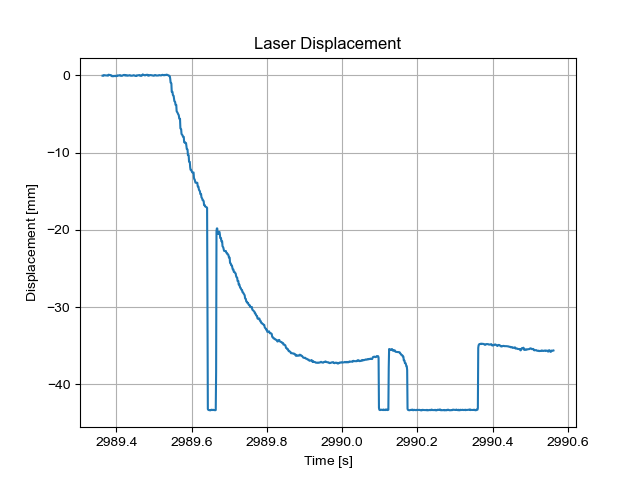
\includegraphics[width=0.45\linewidth]{pics/perfectlaser.png}} 
\subcaptionbox{A usable laser reading,\\test 2018-12-04\_Rfrs\_50\_0,3\_2 
\label{fig:goodlaser}}
{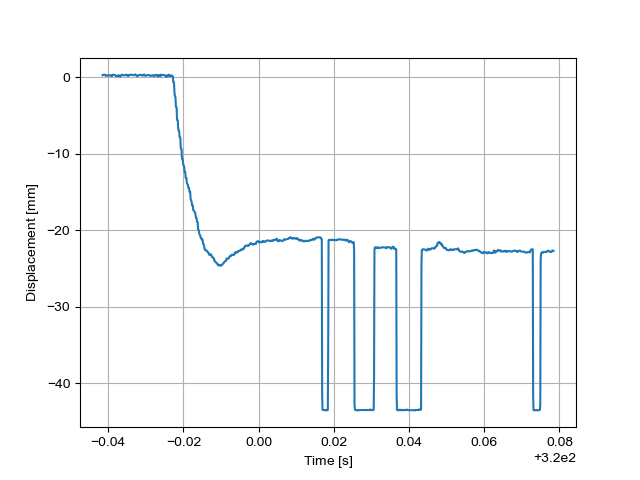
\includegraphics[width=0.45\linewidth]{pics/goodlaser.png}} 
\subcaptionbox{A bad laser reading,\\test 2018-11-09\_Rfrs\_70\_0,5 
\label{fig:badlaser}} 
{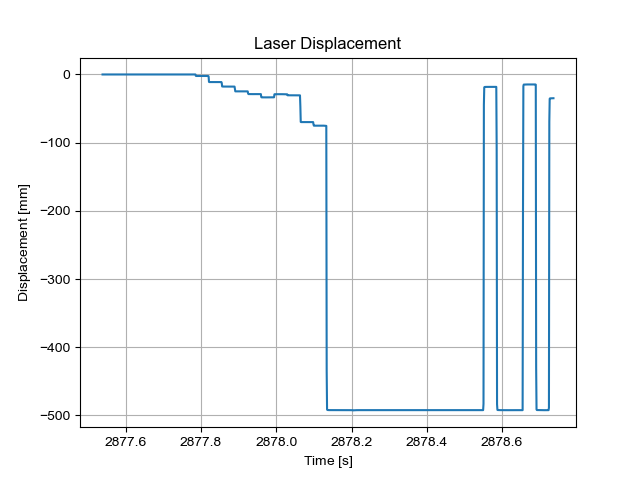
\includegraphics[width=0.45\linewidth]{pics/badlaser.png}} 
\subcaptionbox{An ejected particle (\(v = 2~\rfrac{m}{s}\)) caught in the beam,\\test 2018-12-04\_Rfrs\_50\_0,3 
\label{fig:weirdlaser}}
{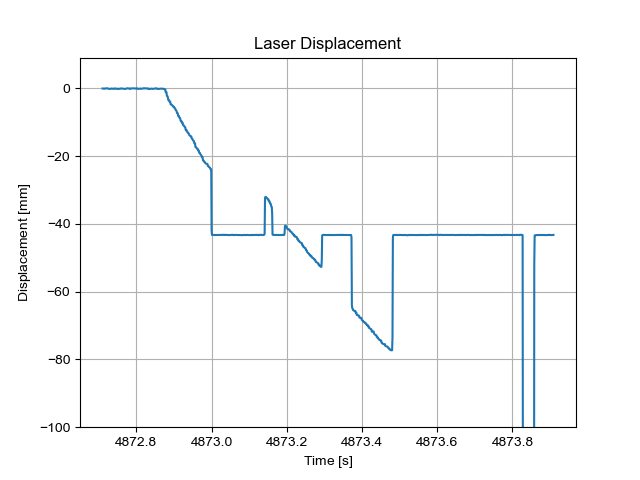
\includegraphics[width=0.45\linewidth]{pics/weirdlaser.png}} 
\caption{Problems with laser sensor readings} \label{fig:laser} 
\end{figure}

\begin{figure} 
\centering
\subcaptionbox{Parallel tape after a test
    \label{fig:riptape}}{
    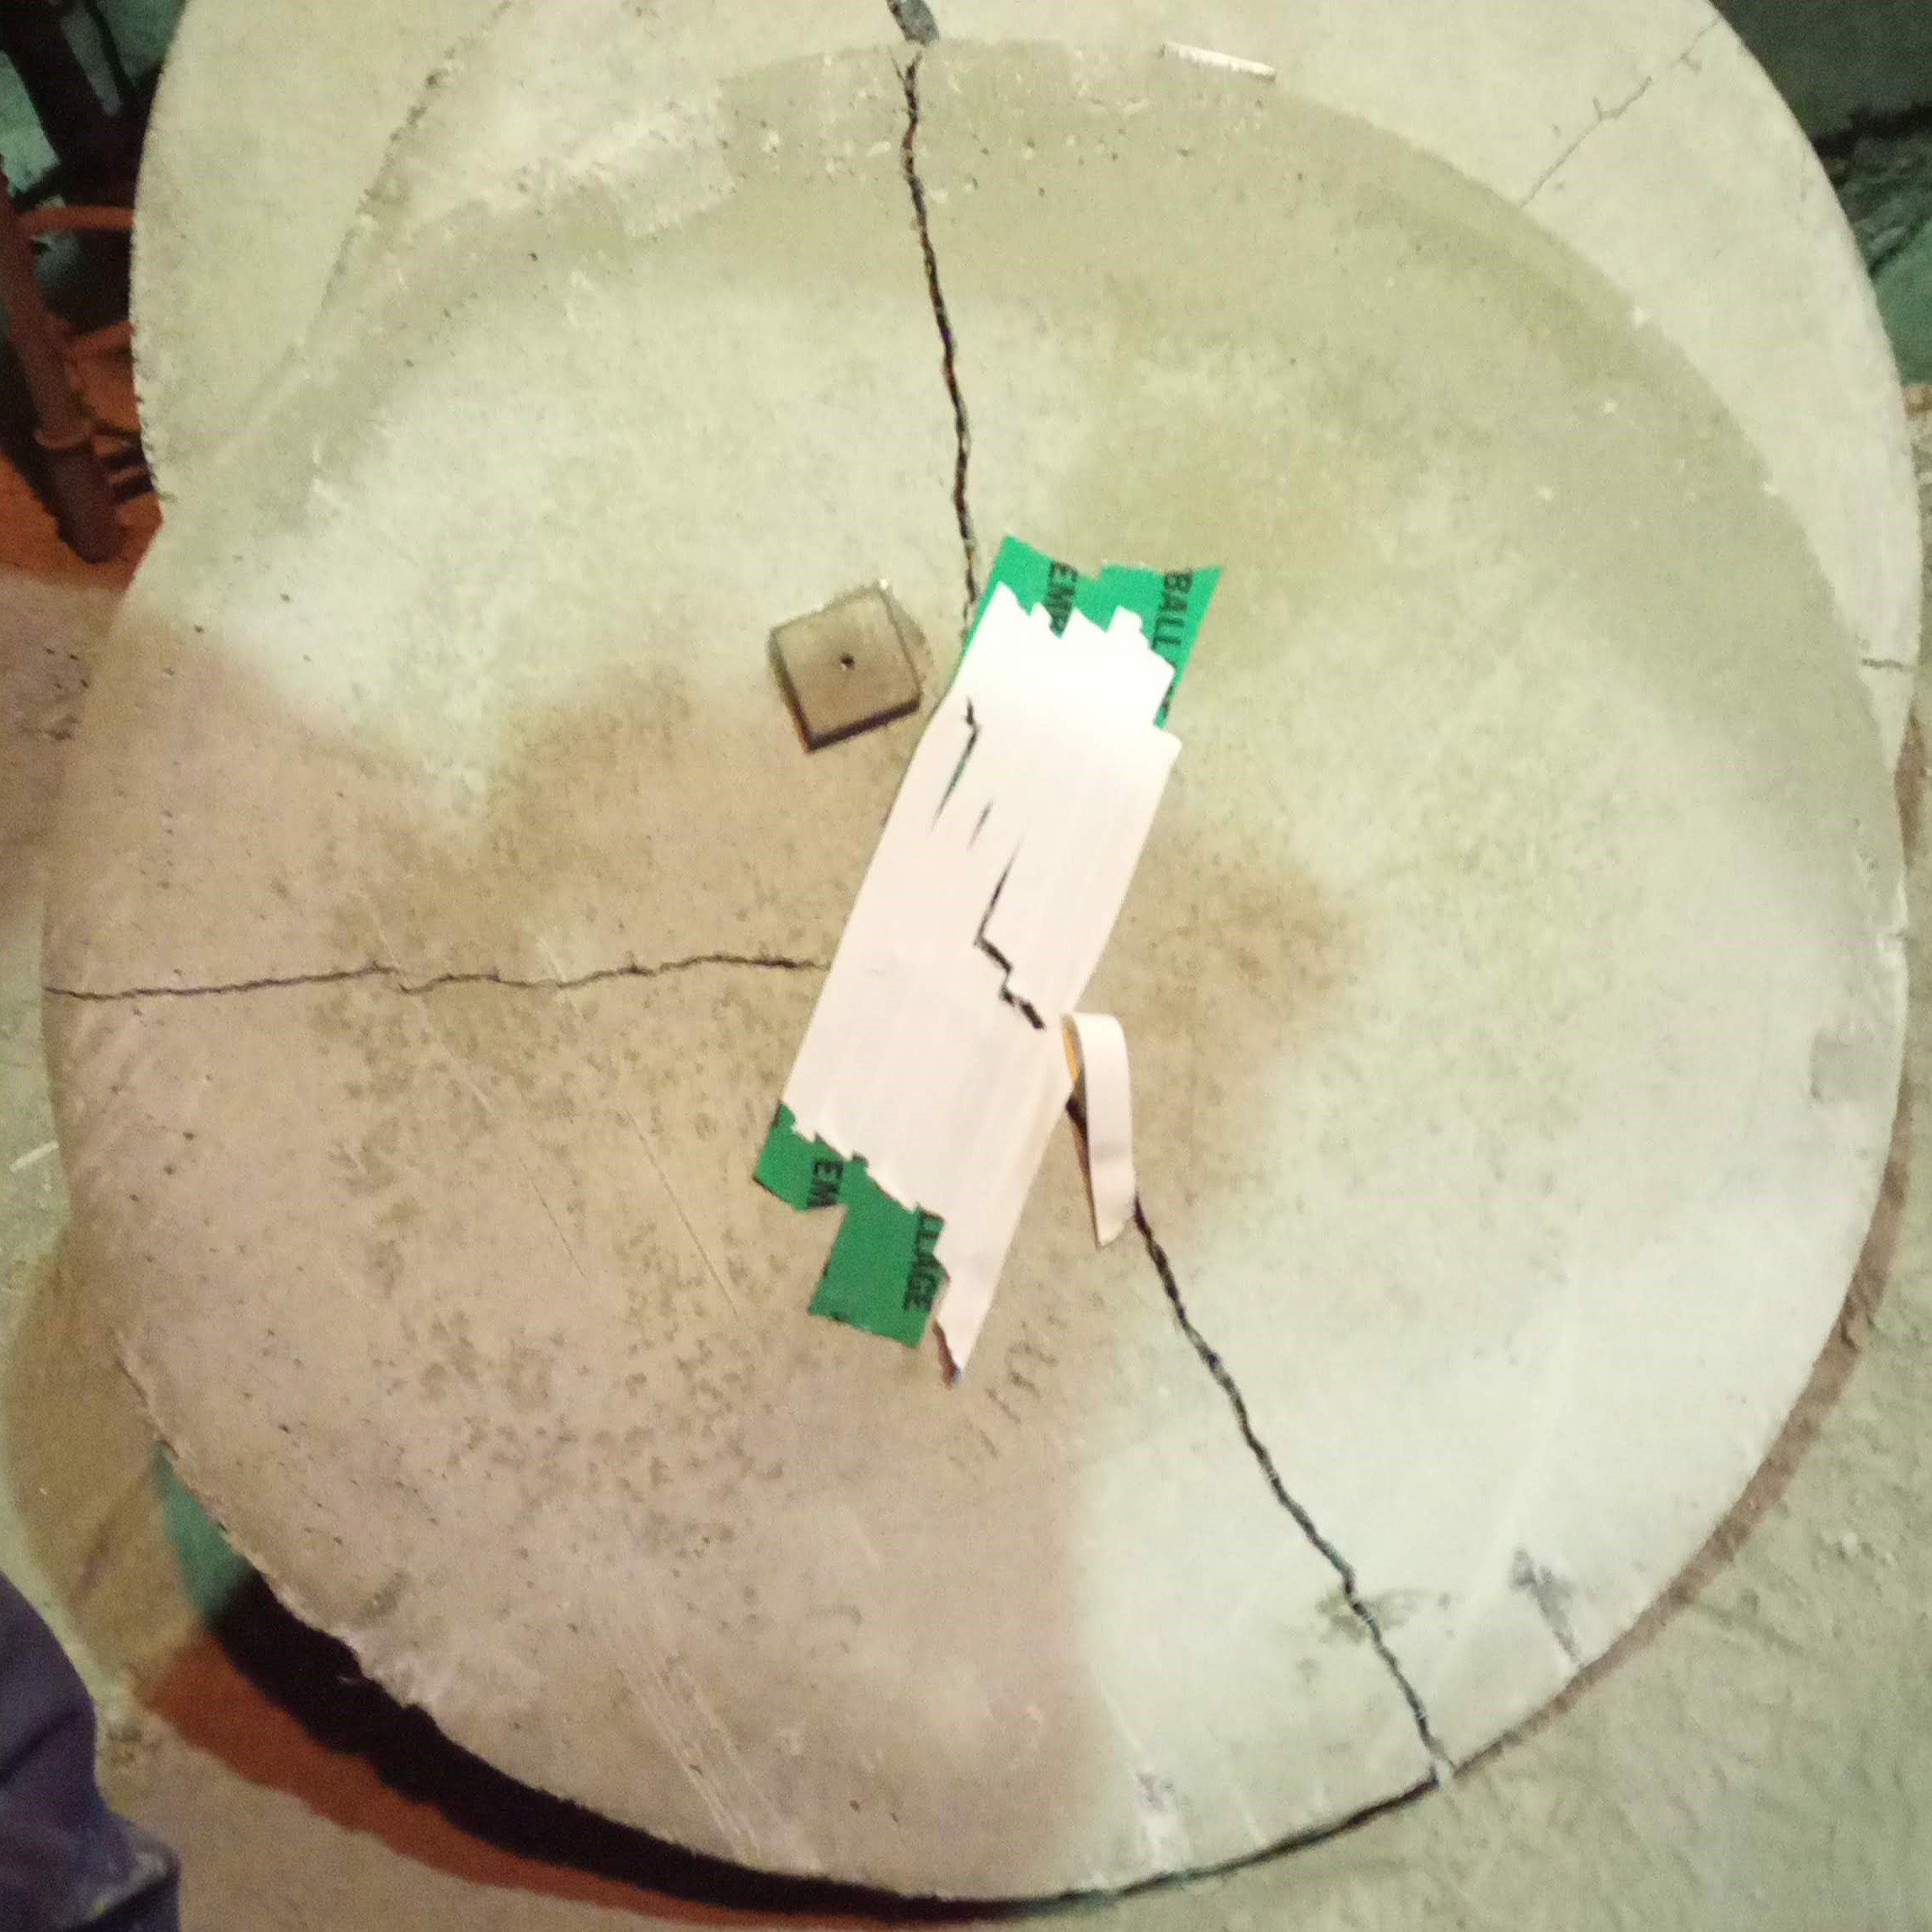
\includegraphics[width=0.45\linewidth]{pics/parallel.jpg}}
\subcaptionbox{Basket weave tape after a test\label{fig:tape}}{
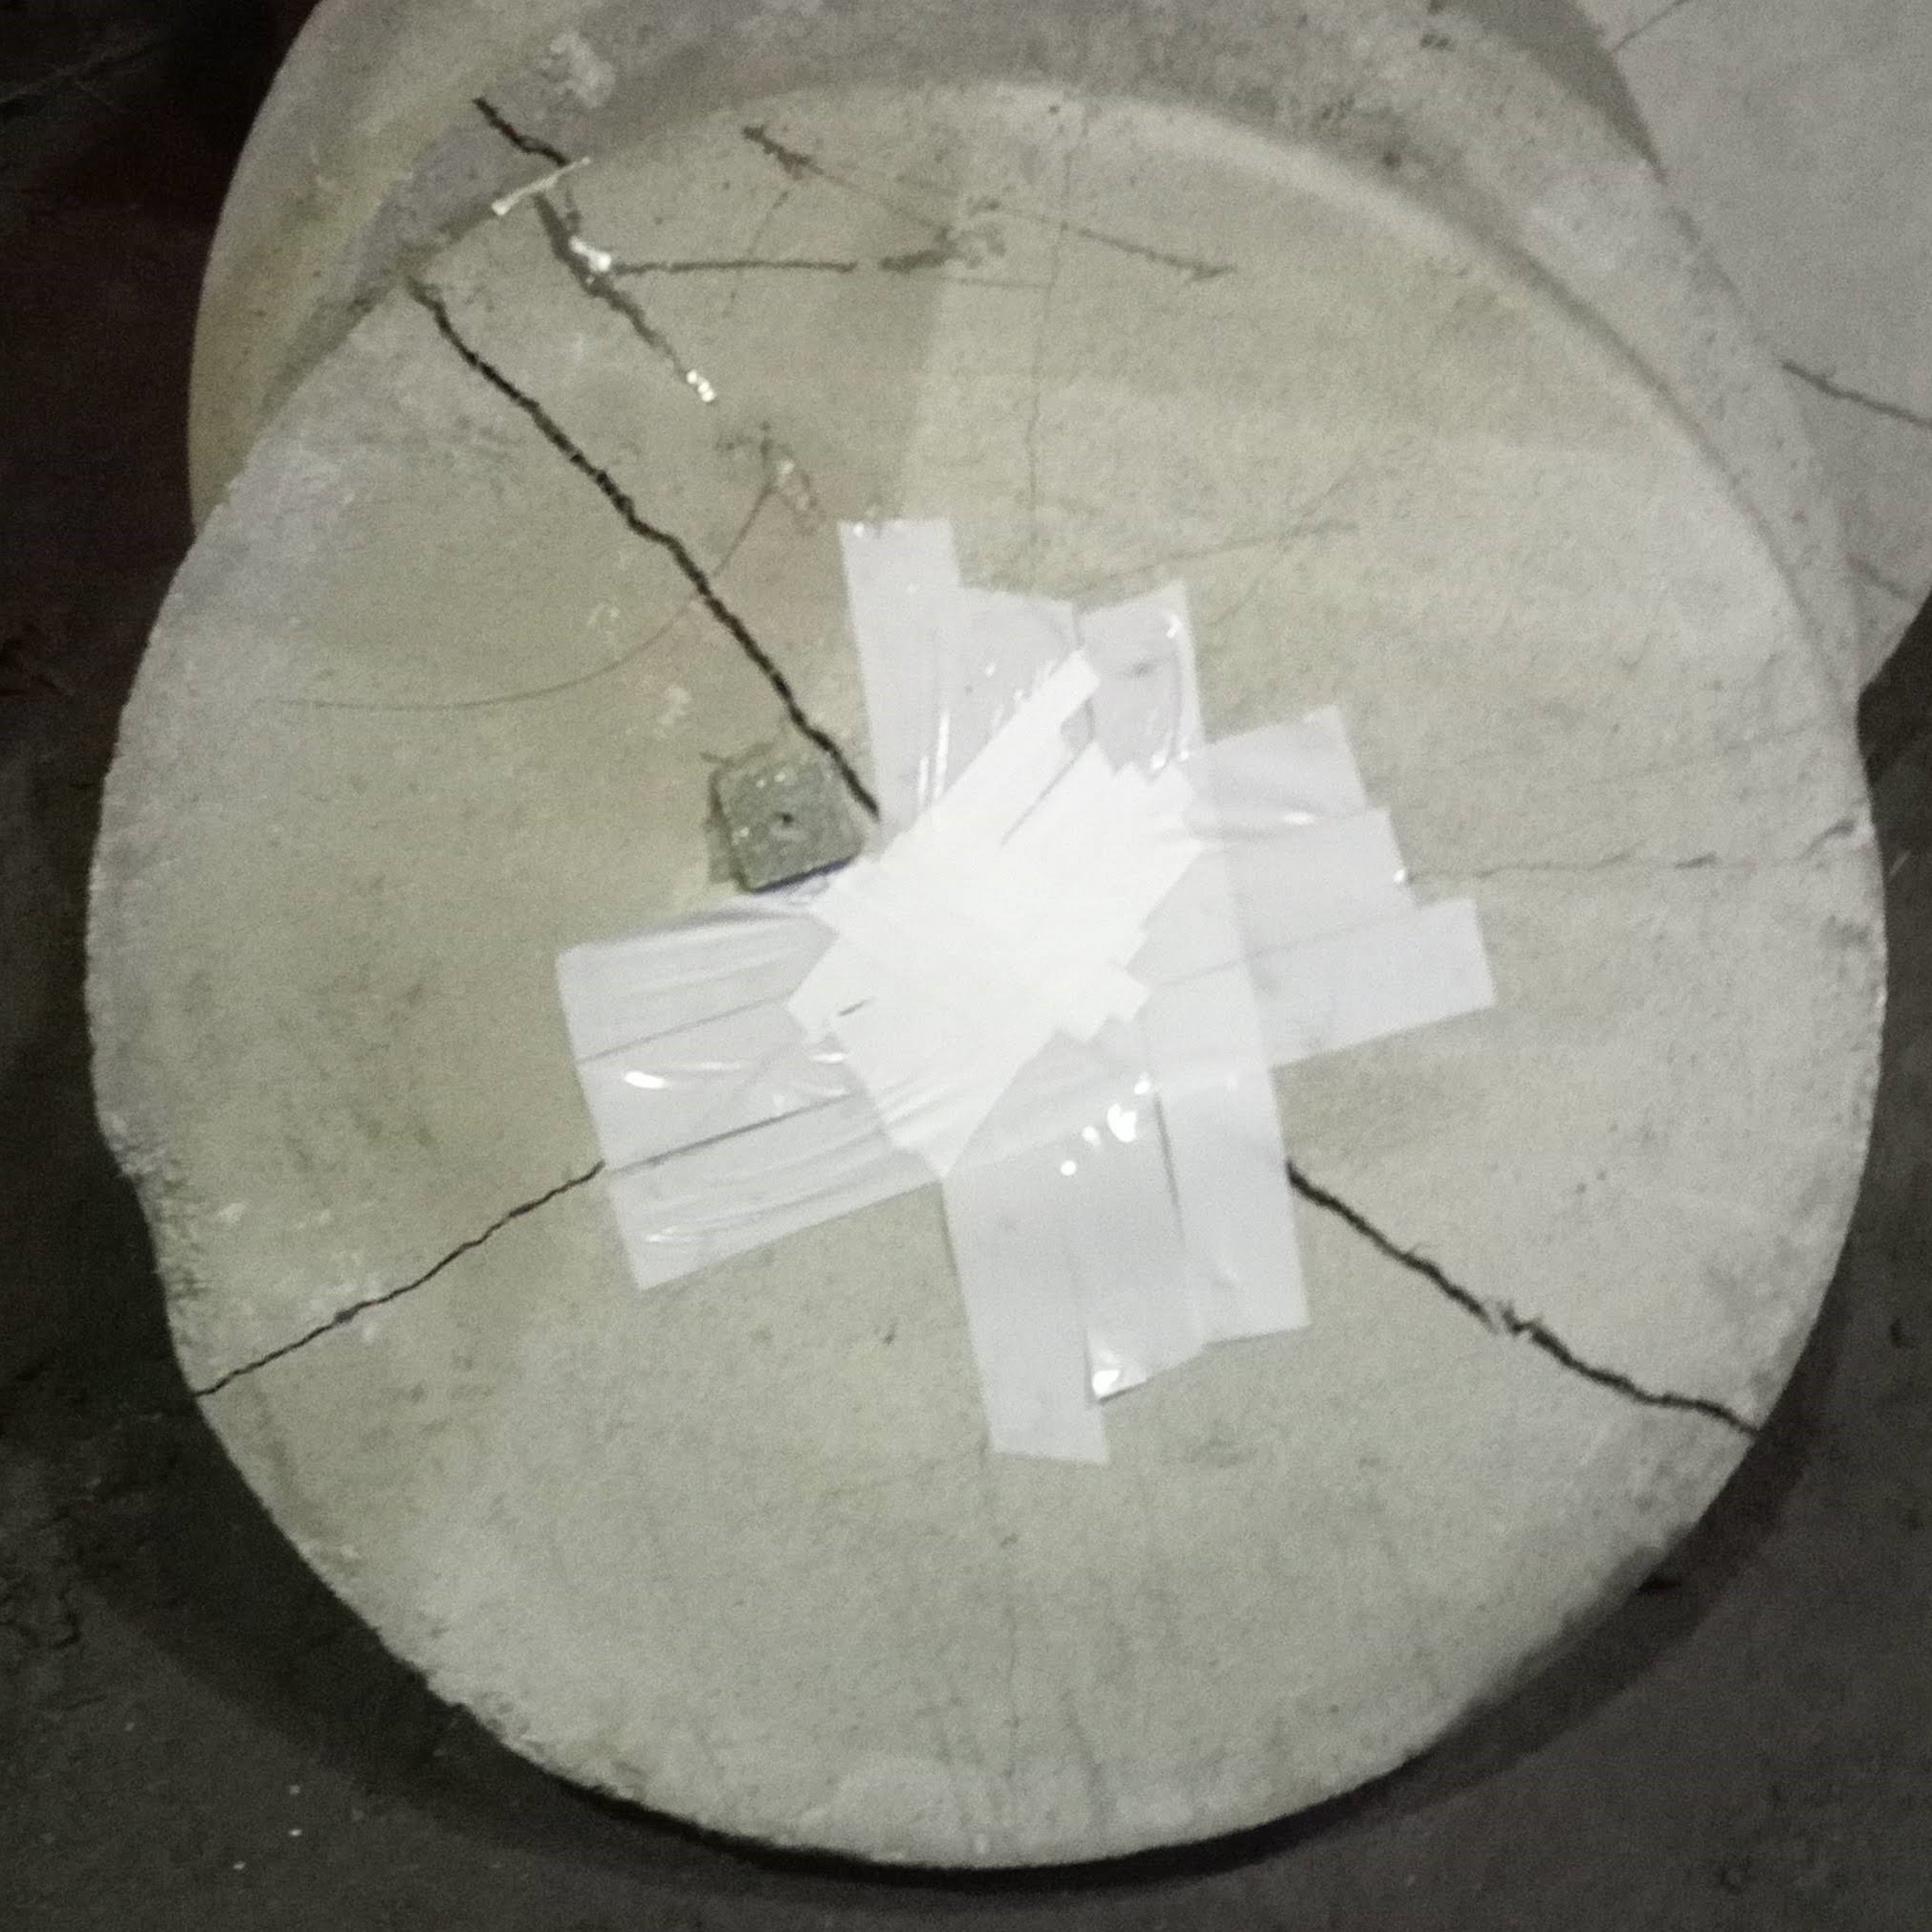
\includegraphics[width = 0.45\linewidth]{pics/basket.jpg}}

\caption{Different ways of applying tape to a sample}
\label{fig:beauty_tape}
\end{figure}

To contain the dust and create a smooth surface for the laser tape was glued on the samples. Two ways of gluing the tape on the concrete were tried.
Firstly the tape was applied in one layer in parallel strips. These were over stretched and ripped. See \autoref{fig:riptape}. Even though the tape ripped it reduced the development of dust significantly. 

Secondly the tape was applied in a basket weave pattern. With strips alternating vertically and horizontally crossing each other. See \autoref{fig:tape}.
This setup did not rip but it was prone to detaching from the sample.

If the displacement were to be measured using computer vision or photogrammetry in the future, covering the entire surface of the sample with a thin film of latex of another flexible stabiliser might reduce the dust production enough to yield usable results. For this thesis using photogrammetry to measure the displacement was considered but as the cameras would have to be placed above the sample and the expected deformations on top and on bottom are not the same this idea was discarded.


The high speed camera was the redundant sensor for measuring the deformation of the sample and it suffered a few failures as well.

\subsection{Increasing the Reliability of the High Speed Camera}

The failures of the high speed camera were all caused by operator mistakes. A check list was implemented to keep such errors from happening.

Even though the sensors malfunctioned at times enough data could be collected to get results.

\section{Results of Round Sample Tests}

The round samples were the first to be tested. The additional accelerometers attached directly to the sample yielded interesting insights into the way the impact propagated through the sample.

\subsection{Additional Accelerometer}

In \autoref{tab:acc_compare} the acceleration measured on the drop weight and on the sample are compared. The acceleration measured on the sample 2019-04-16\_Rfrs\_75\_0,5 is significantly higher because the impact velocity was much higher.

The drop weight appears to undergo overwhelmingly positive acceleration while the sample experiences both positive and negative acceleration. This is not surprising as the drop weight is already accelerated to the impact velocity before impact and has to decelerate down to zero. The sample is first accelerated downward and outward and deforming elastically before returning to its plastic post deformation shape.  The acceleration measured on the sample appears to be mostly biased towards positive acceleration. 

\begin{table}
    \centering
    \begin{tabular}{lllllll}
    \toprule
    Sample number		&   \multicolumn{2}{l}{Drop weight}	& \multicolumn{4}{c}{Sample} \\
    \cmidrule{4 - 7}
    			&		&							& \multicolumn{2}{l}{Vertical}	& \multicolumn{2}{l}{Horizontal}    \\
    \midrule
    5  & 1718,23 & - 120,42 & 3384,14 & - 2027,52 & &\\
    15 & 1389,15 & - 55,74 & 4919,99 & - 3825,53 & &\\
    16 & 3963,18 & - 931,50 & 1507,00 & -964,91 & 525,13 & - 564,48\\
    %\multicolumn{2}{c}{Drop weight} &   \multicolumn{2}{c}{Vertical}    &   \multicolumn{2}{c}{Horizontal}\\
    %\midrule
    %3963.18 & - 931.50 & 1507,00 & -964,91 & 525,13 & - 564,48\\
    \bottomrule
    \end{tabular}
    \caption{Comparing the acceleration [$\frac{\text{m}}{\text{s}^2}$] measured on drop weight to the acceleration measured directly on the sample}
    \label{tab:acc_compare}
\end{table}


\begin{figure} 
\centering 
\subcaptionbox{Bouncing as measured by the accelerometer \label{fig:accelBounce}}
{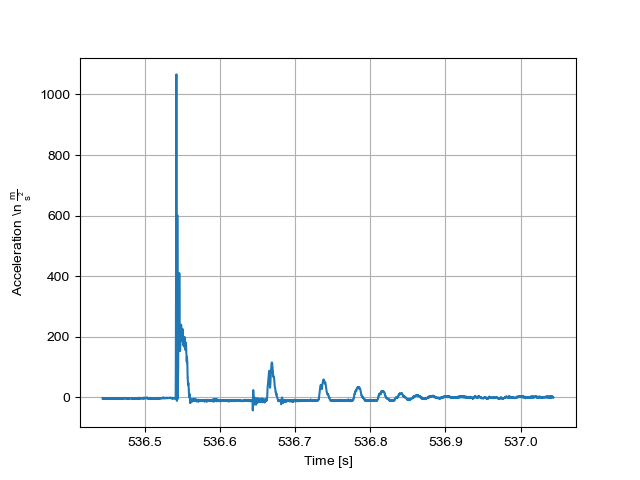
\includegraphics[width=0.45\linewidth]{pics/accelbounce.png}} 
\subcaptionbox{Bouncing as measured by the load cell \label{fig:loadBounce}} 
{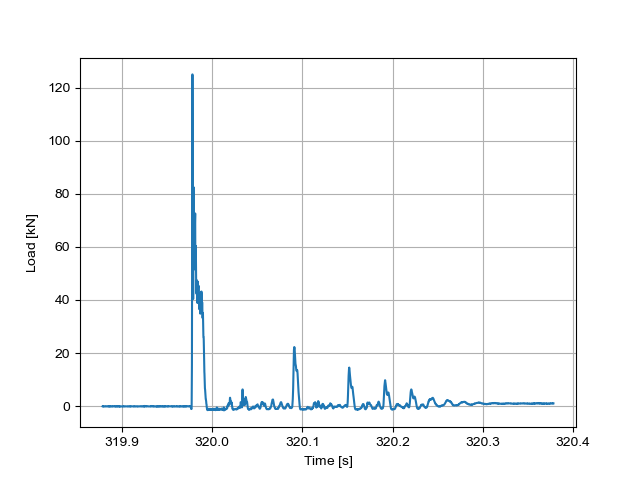
\includegraphics[width=0.45\linewidth]{pics/loadbounce.png}}

\caption{Bouncing of the drop weight after impact}
\label{fig:Bounce} 
\end{figure}

The additional accelerometers yielded interesting data about the behaviour of the sample. The drop weight seems to be reverberating for quite some time (200 ms), while the sample quickly settles in its new shape (2 ms). The accelerometer on the sample registers larger accelerations than the the sensor on the drop weight as displayed in \autoref{fig:acccom}. Note that 2019-02-20\_Rfrs\_100\_1,0 broke during testing  and 2019-04-16\_Rfrs\_75\_0,5 only cracked. This explains the longer vibration time of 2019-02-20\_Rfrs\_100\_1,0. From this graphic it is obvious that the vertical acceleration and the horizontal acceleration both look similar to each other.

\begin{figure}
    \centering
    \subcaptionbox{Step 0: Before impact \label{fig:bounce0}}
    {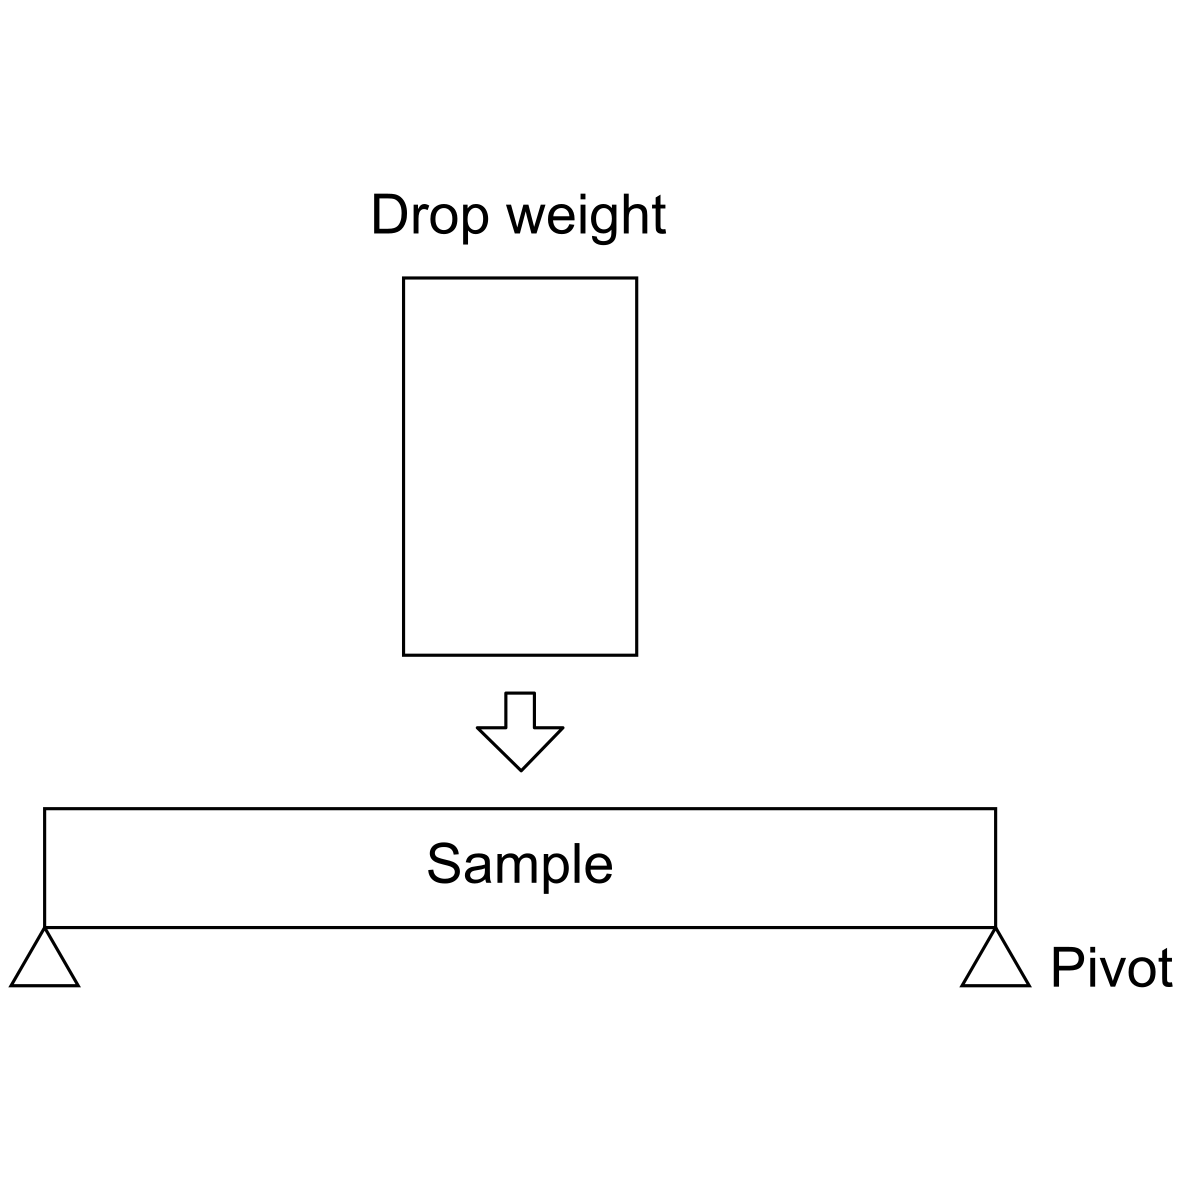
\includegraphics[width = 0.45\linewidth]{pics/bounce_0.png}}
    \subcaptionbox{Step 1: Sample deforms plastic and elastic \label{fig:bounce1}}
    {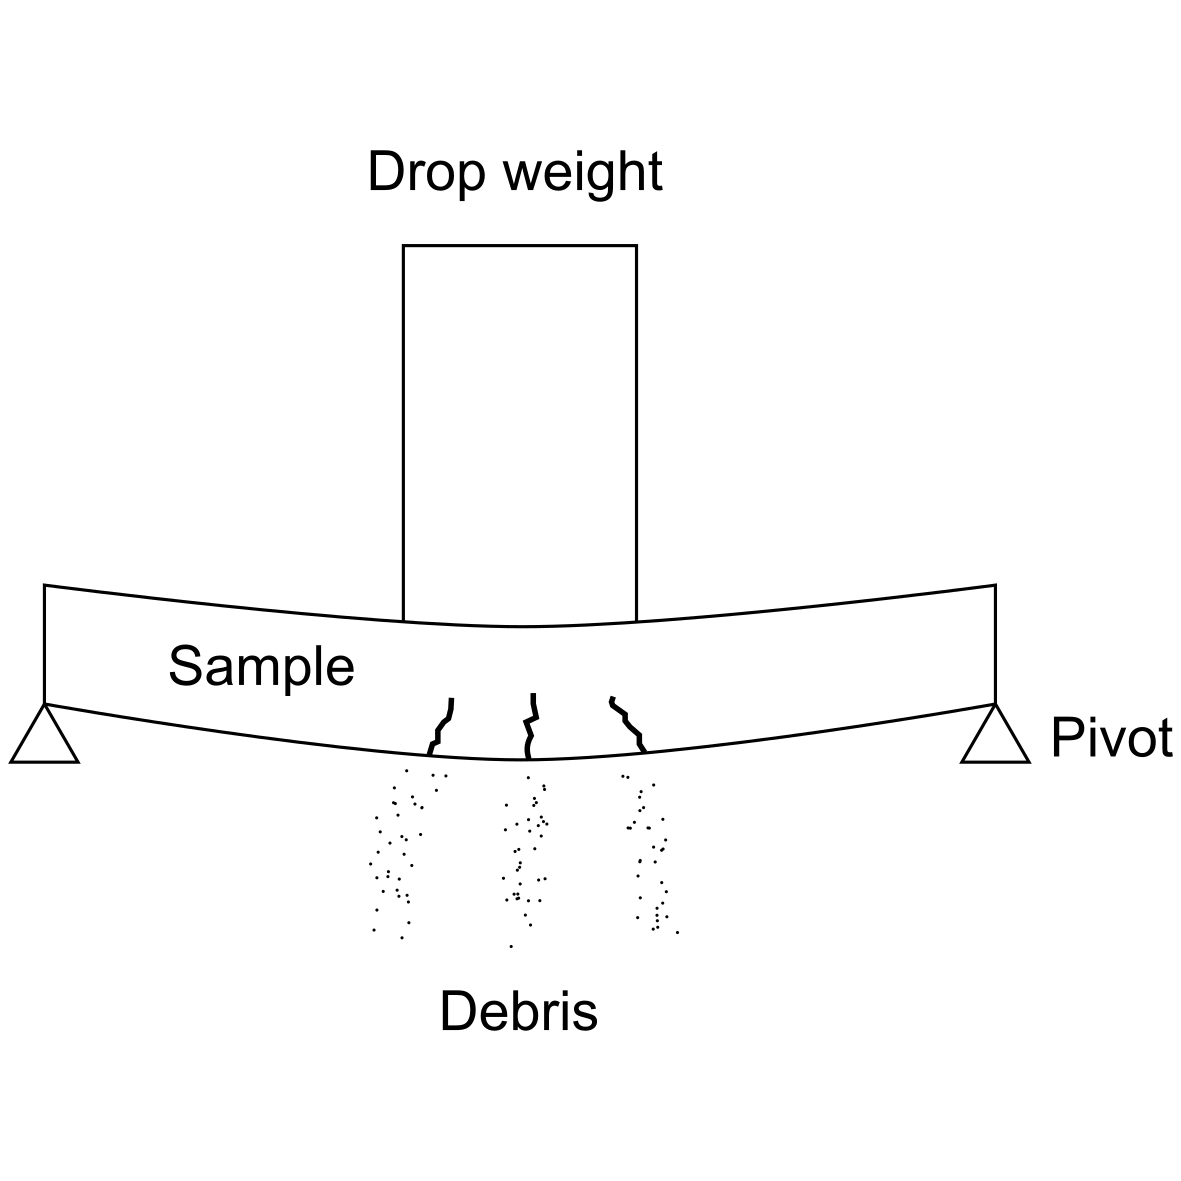
\includegraphics[width = 0.45\linewidth]{pics/bounce_1.png}}
    
    \subcaptionbox{Step 2: Elastic deformation energy is \\ released, sample and drop weight jump \label{fig:bounce2}}
    {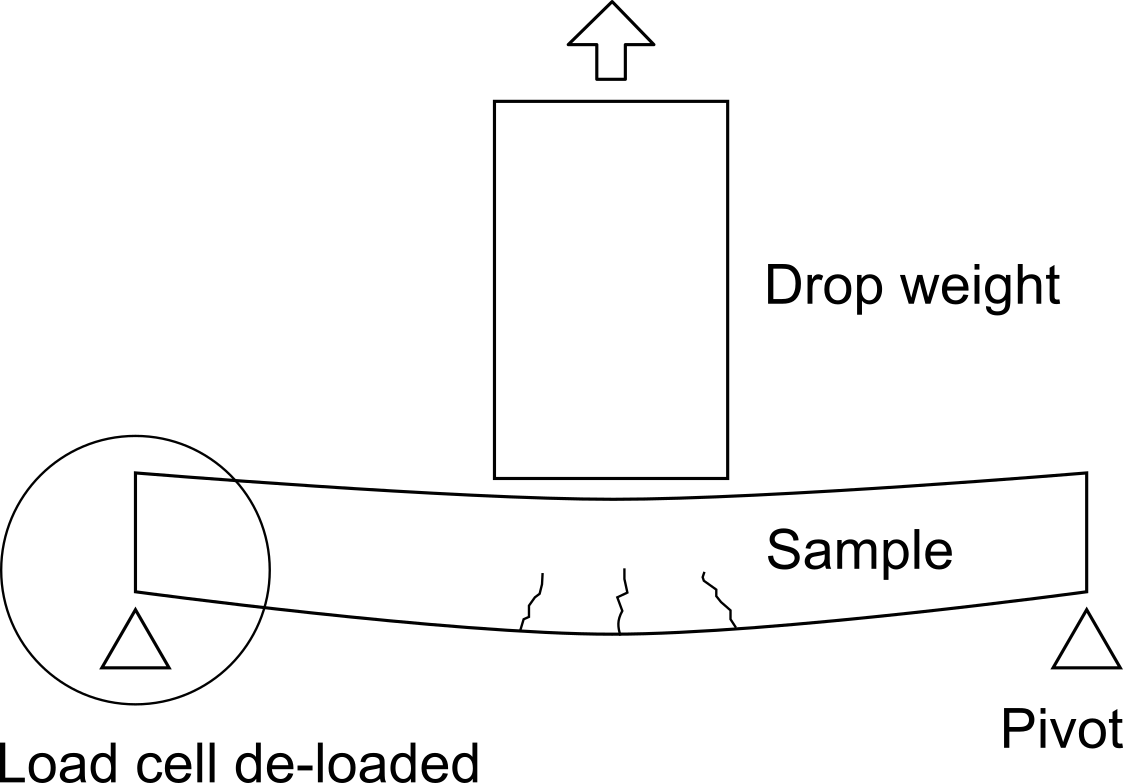
\includegraphics[width = 0.45\linewidth]{pics/bounce_2.png}}
    \subcaptionbox{Step 3: Sample and drop weight drop again \label{fig:bounce3}}
    {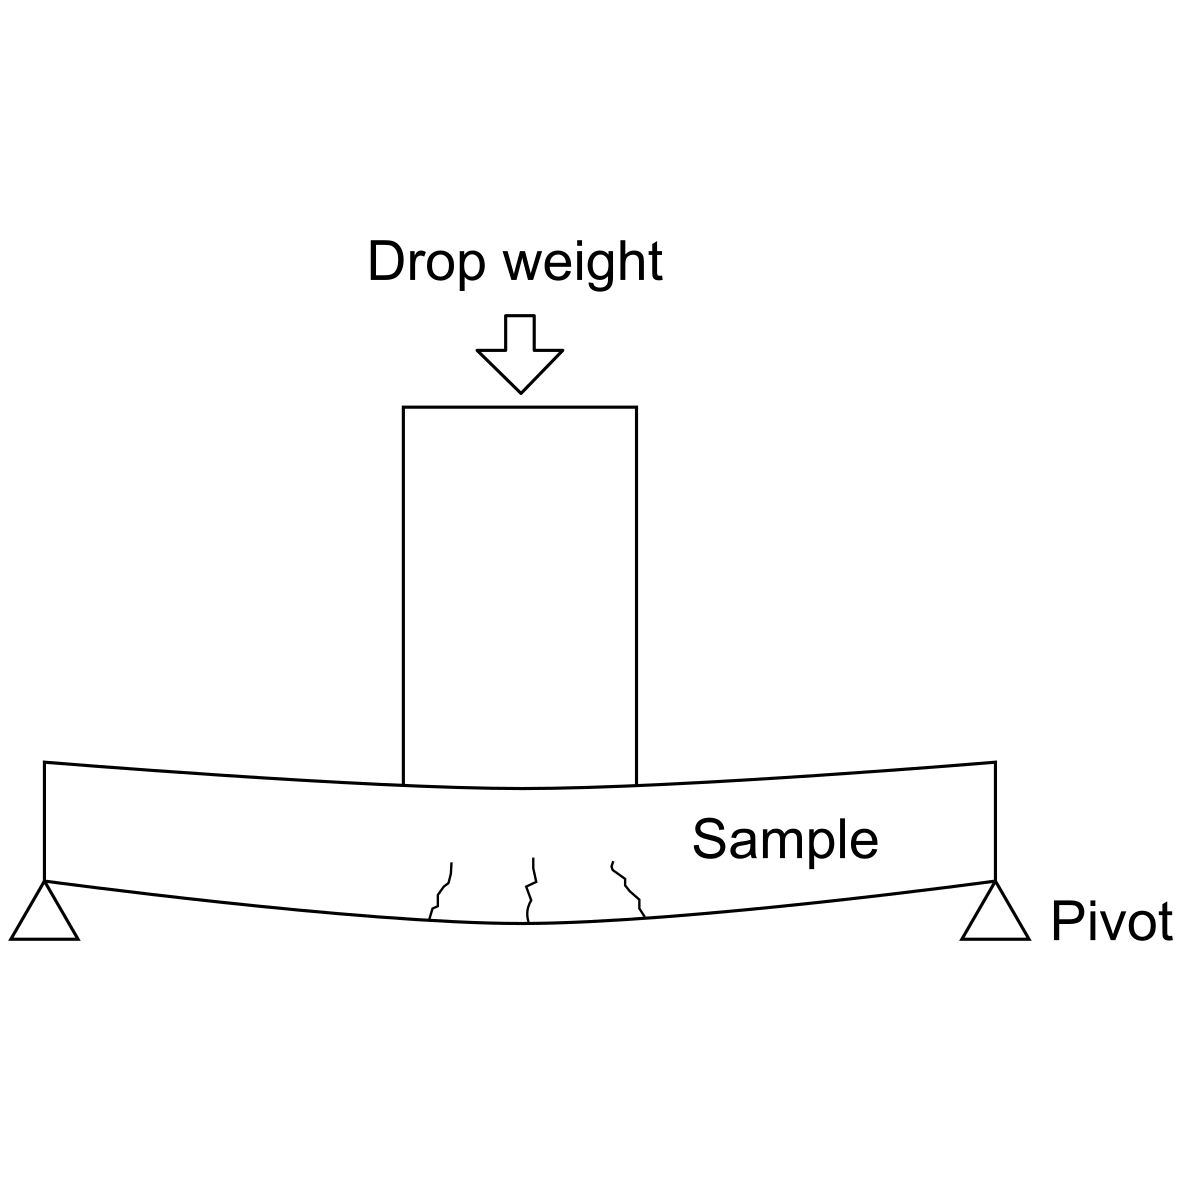
\includegraphics[width = 0.45\linewidth]{pics/bounce_3.png}}
    \caption{The mechanism behind the bouncing of the sample}
    \label{fig:bounce}
\end{figure}

In the high speed footage taken of sample 2019-08-19\_Rfrs+t\_75\_1,0 it appears that the entire sample jumps upwards a few millimeters following the initial impact. The bouncing appears to follow a simple pattern. See \autoref{fig:bounce}.

In \autoref{fig:bounce1} the initial impact is displayed the sample cracks and debris is expelled from the cracks. The sample experiences maximum deformations at this point and the  vast majority of the cracks is formed. 

The elastic deformation energy is released again after the initial impact and both sample and drop weight bounce upwards and either complete de-load the load cells or at least reduce the load on them. The drop weight jumps slightly higher than the sample. In the high speed camera footage it looks as if the sample has already settled into its new position when it is struck by the second impact. 
See \autoref{fig:bounce2}.

Sample and drop weight fall back down. The sample experiences more elastic and plastic deformation. This is displayed in \autoref{fig:bounce3}.

Step 2 and 3 repeat until the entire impact energy has been dissipated.

Some discord exists between readings of the additional accelerometers and the high speed camera. The accelerometers show that the acceleration of the sample stabilizes very quickly (2 ms) while it is bouncing for a significant amount of time (400 ms) on the high speed camera footage. No test with good high speed camera coverage and additional accelerometers exists. This makes this phenomenon even harder to explain.

Initially it was supposed that the accelerometer on the sample could be used to calculate the displacement. The measurements showed a lot of zero drift an zero offset after integrating them to get the impact velocity and the displacement. These errors had to be removed in post processing. As no sample has working additional accelerometers and displacement measurements it was not possible to calibrate the double integrated curves. They were deemed to unreliable to use in this analysis.

\begin{figure}
    \centering
\subcaptionbox
{Acceleration measured on drop weight for 2019-02-20\_Rfrs\_100\_1,0
\label{fig:accdropweight1}}
{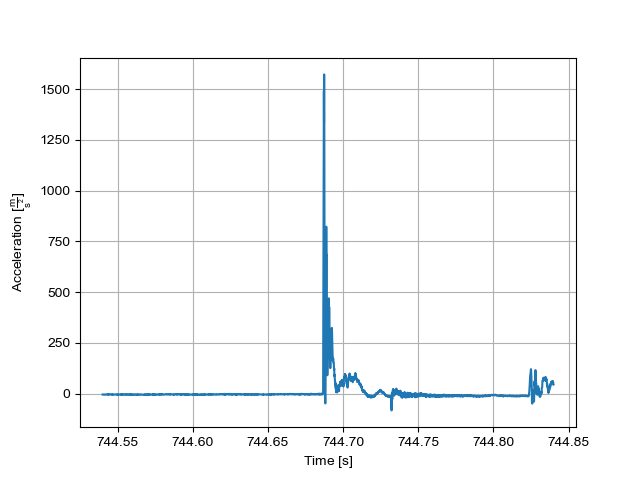
\includegraphics[width = 0.45\linewidth]{graph/2019-02-20_Rfrs_100_1,0.png}}
\subcaptionbox
{Vertical acceleration measured on sample for 2019-02-20\_Rfrs\_100\_1,0
\label{fig:accvertical1}}
{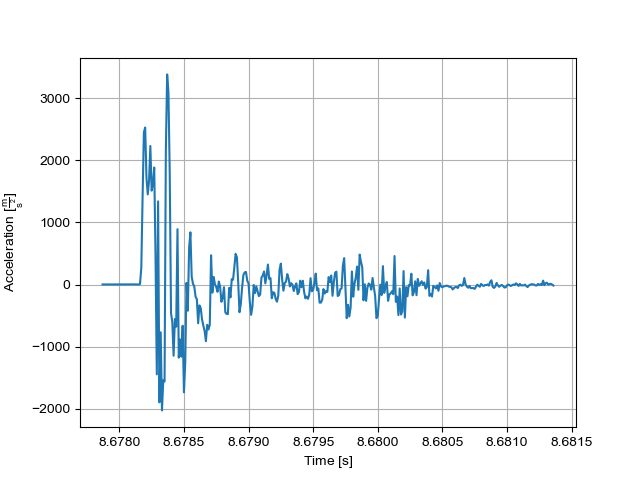
\includegraphics[width = 0.45\linewidth]{graph/2019-02-20_Rfrs_100_1,0_vertical.png}}

%\subcaptionbox
%{Acceleration measured on drop weight for 2019-02-20\_Rfrs\_100\_0,5
%\label{fig:accdropweight2}}
%{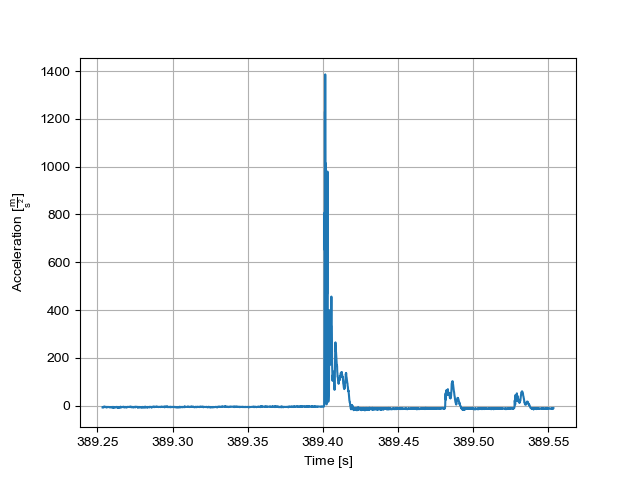
\includegraphics[width = 0.45\linewidth]{graph/2019-02-20_Rfrs_100_0,5.png}}
%\subcaptionbox
%{Vertical acceleration measured on drop sample for 2019-02-20\_Rfrs\_100\_0,5
%\label{fig:accvertical2}}
%{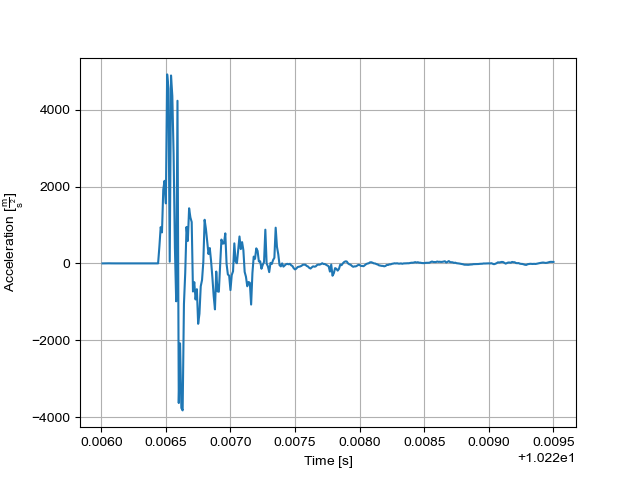
\includegraphics[width = 0.45\linewidth]{graph/2019-02-20_Rfrs_100_0,5_vertical.png}}

\subcaptionbox{Acceleration measured on drop weight for 2019-04-16\_Rfrs\_75\_0,5} {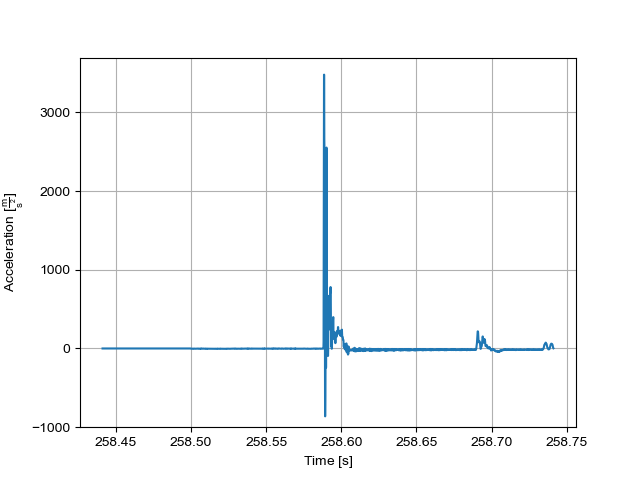
\includegraphics[width=0.45\linewidth]{graph/2019-04-16_Rfrs_75_0,5.png}}
    
\subcaptionbox{Vertical acceleration measured on drop sample for 2019-04-16\_Rfrs\_75\_0,5  }{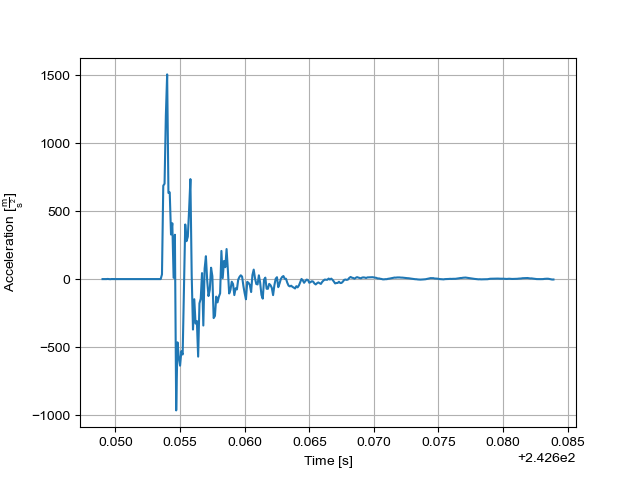
\includegraphics[width=0.45\linewidth]{graph/2019-04-16_Rfrs_75_0,5_vertical.png}}
\subcaptionbox{Horizontal acceleration measured on drop sample for 2019-04-16\_Rfrs\_75\_0,5
}{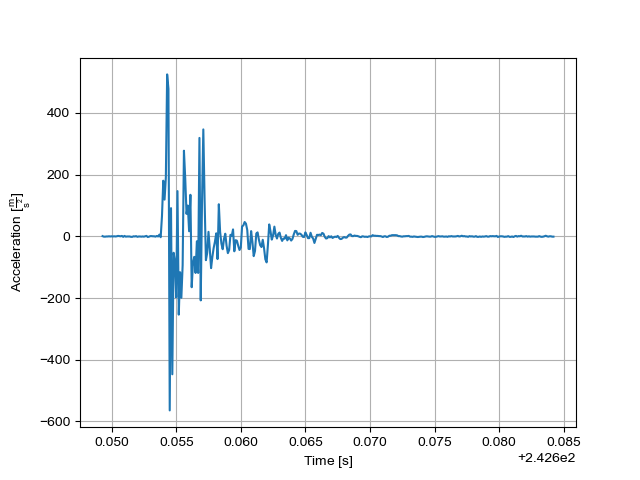
\includegraphics[width=0.45\linewidth]{graph/2019-04-16_Rfrs_75_0,5_horizontal.png}}

\caption{Comparing the measured acceleration on drop weight and on sample}
\label{fig:acccom}
\end{figure}

\begin{figure}
    \centering
    \subcaptionbox{sample 2019-02-20\_Rfs\_75\_0,5}{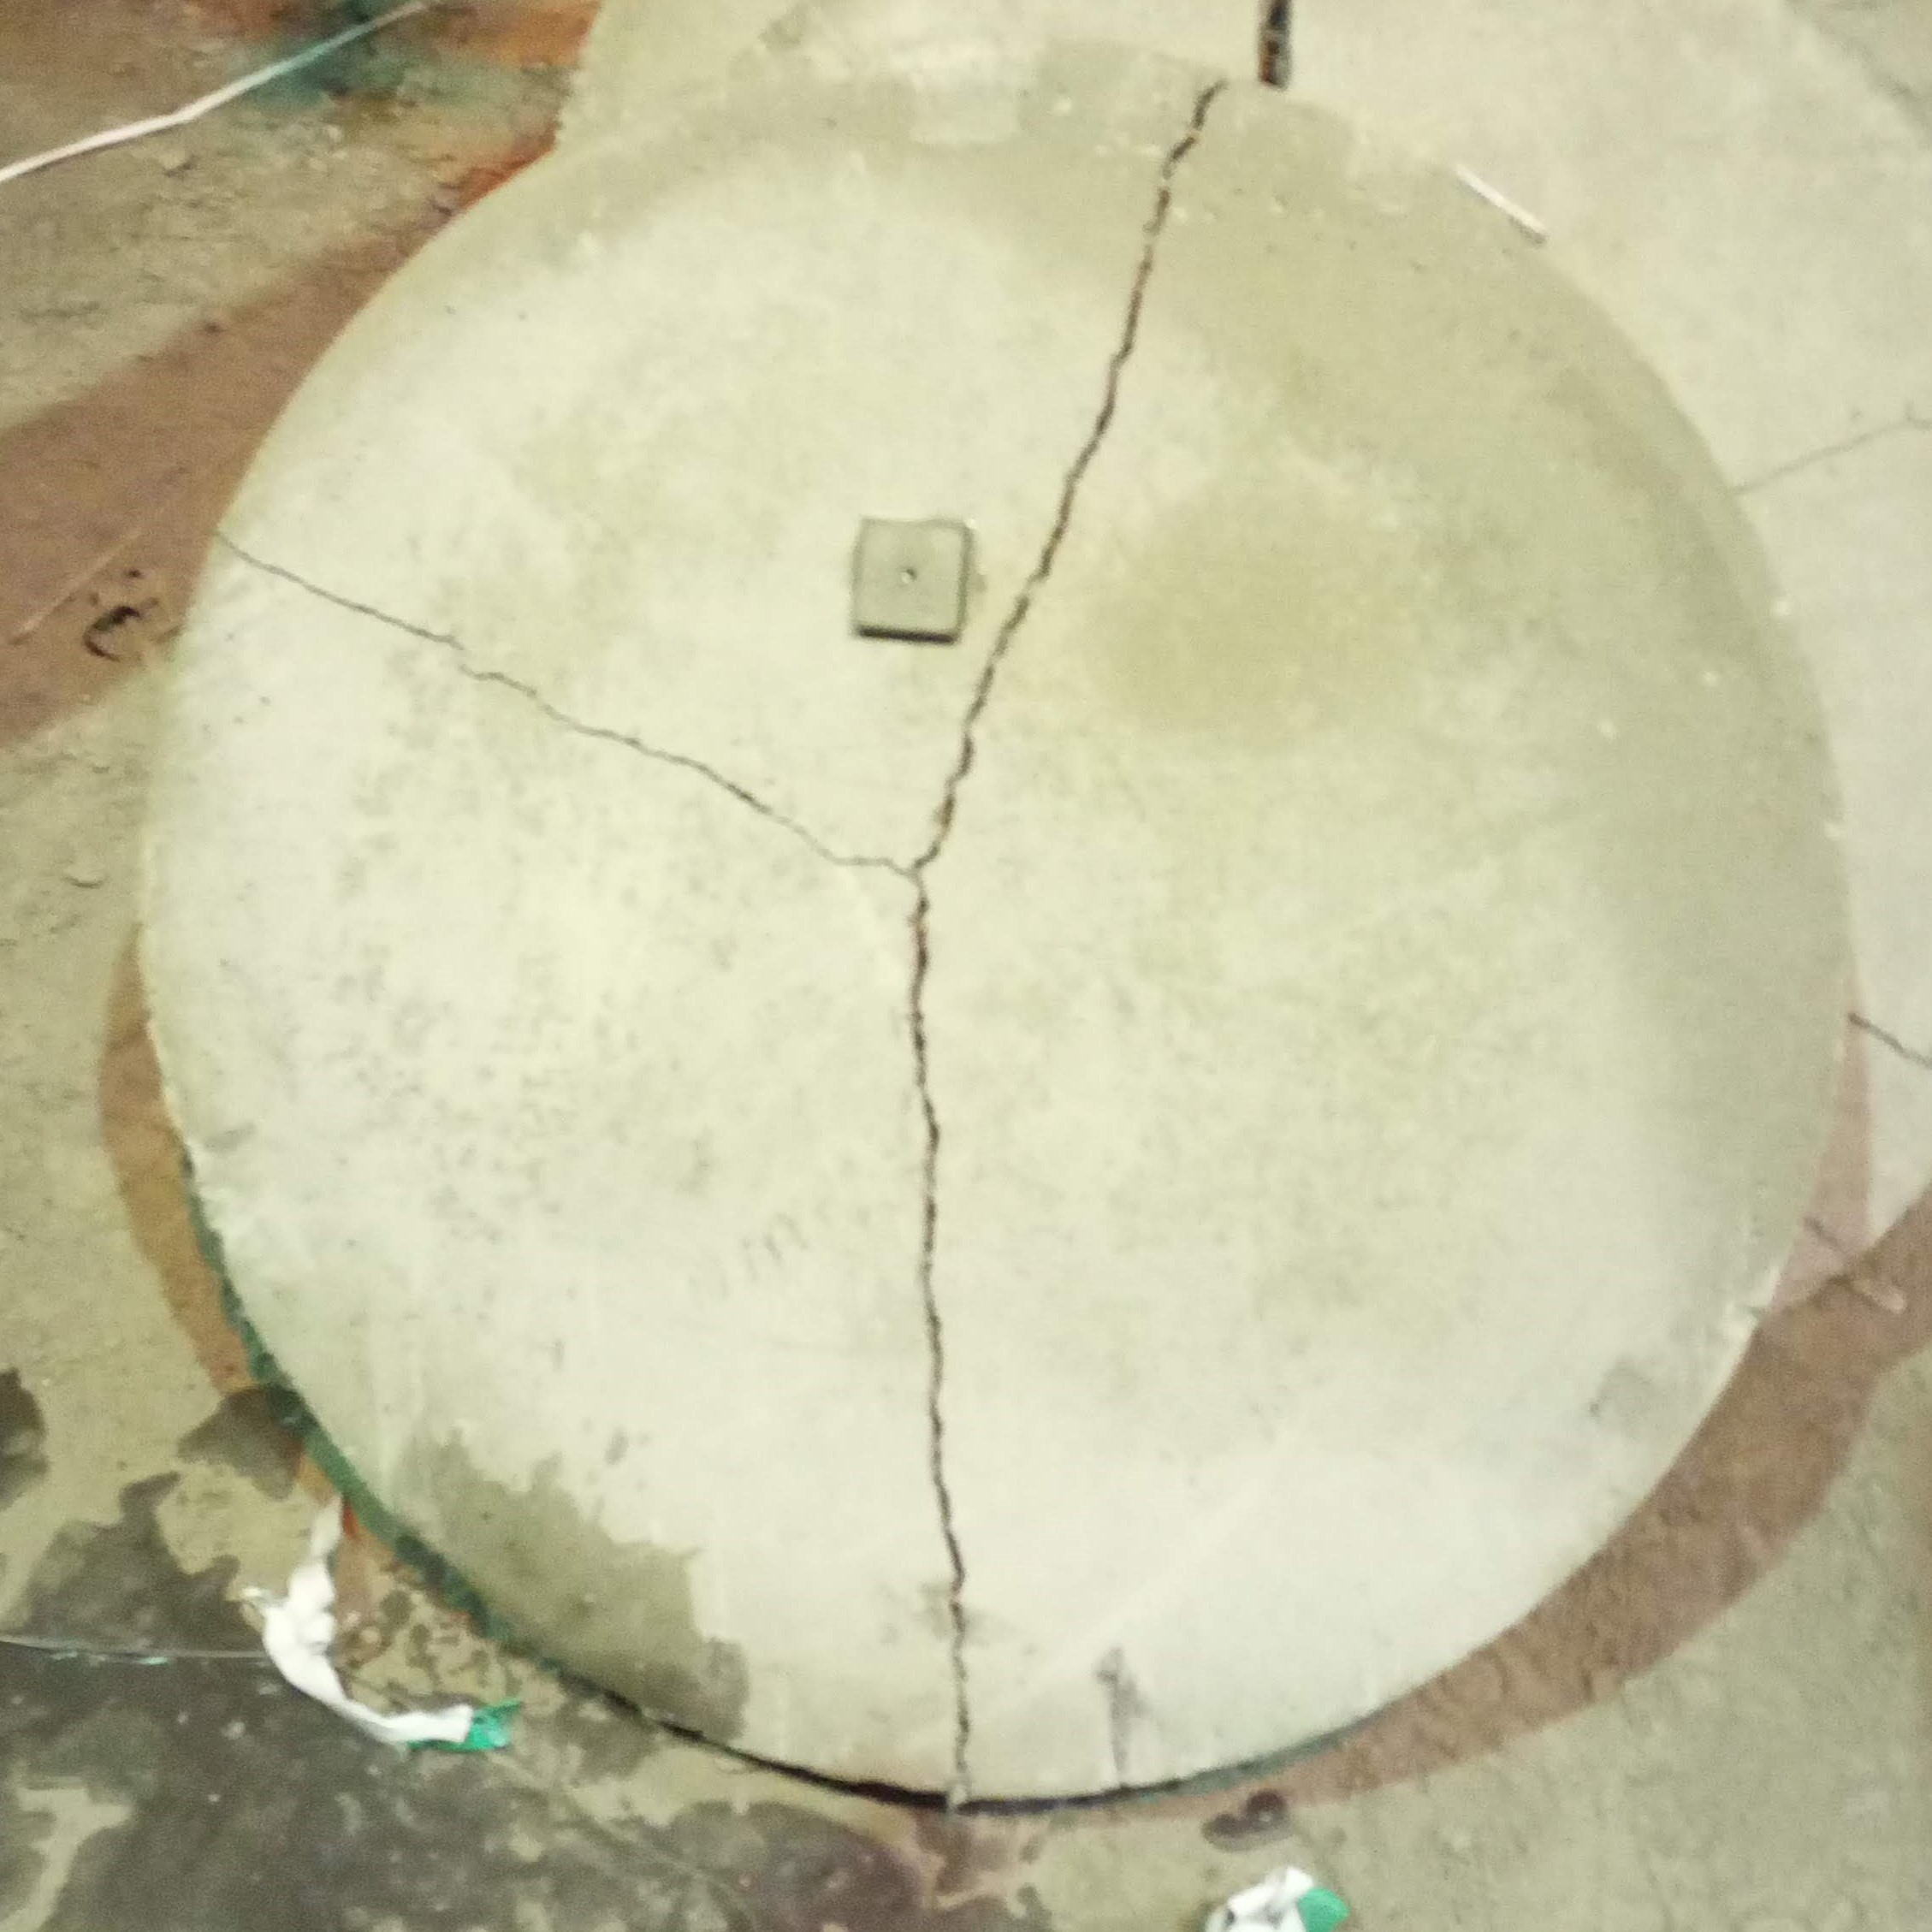
\includegraphics[width = 0.45\linewidth]{appendix/2019-02-20_Rfrs_75_0,5.jpg}}
    \subcaptionbox{sample 2019-04-16\_Rfrs\_75\_0,5}{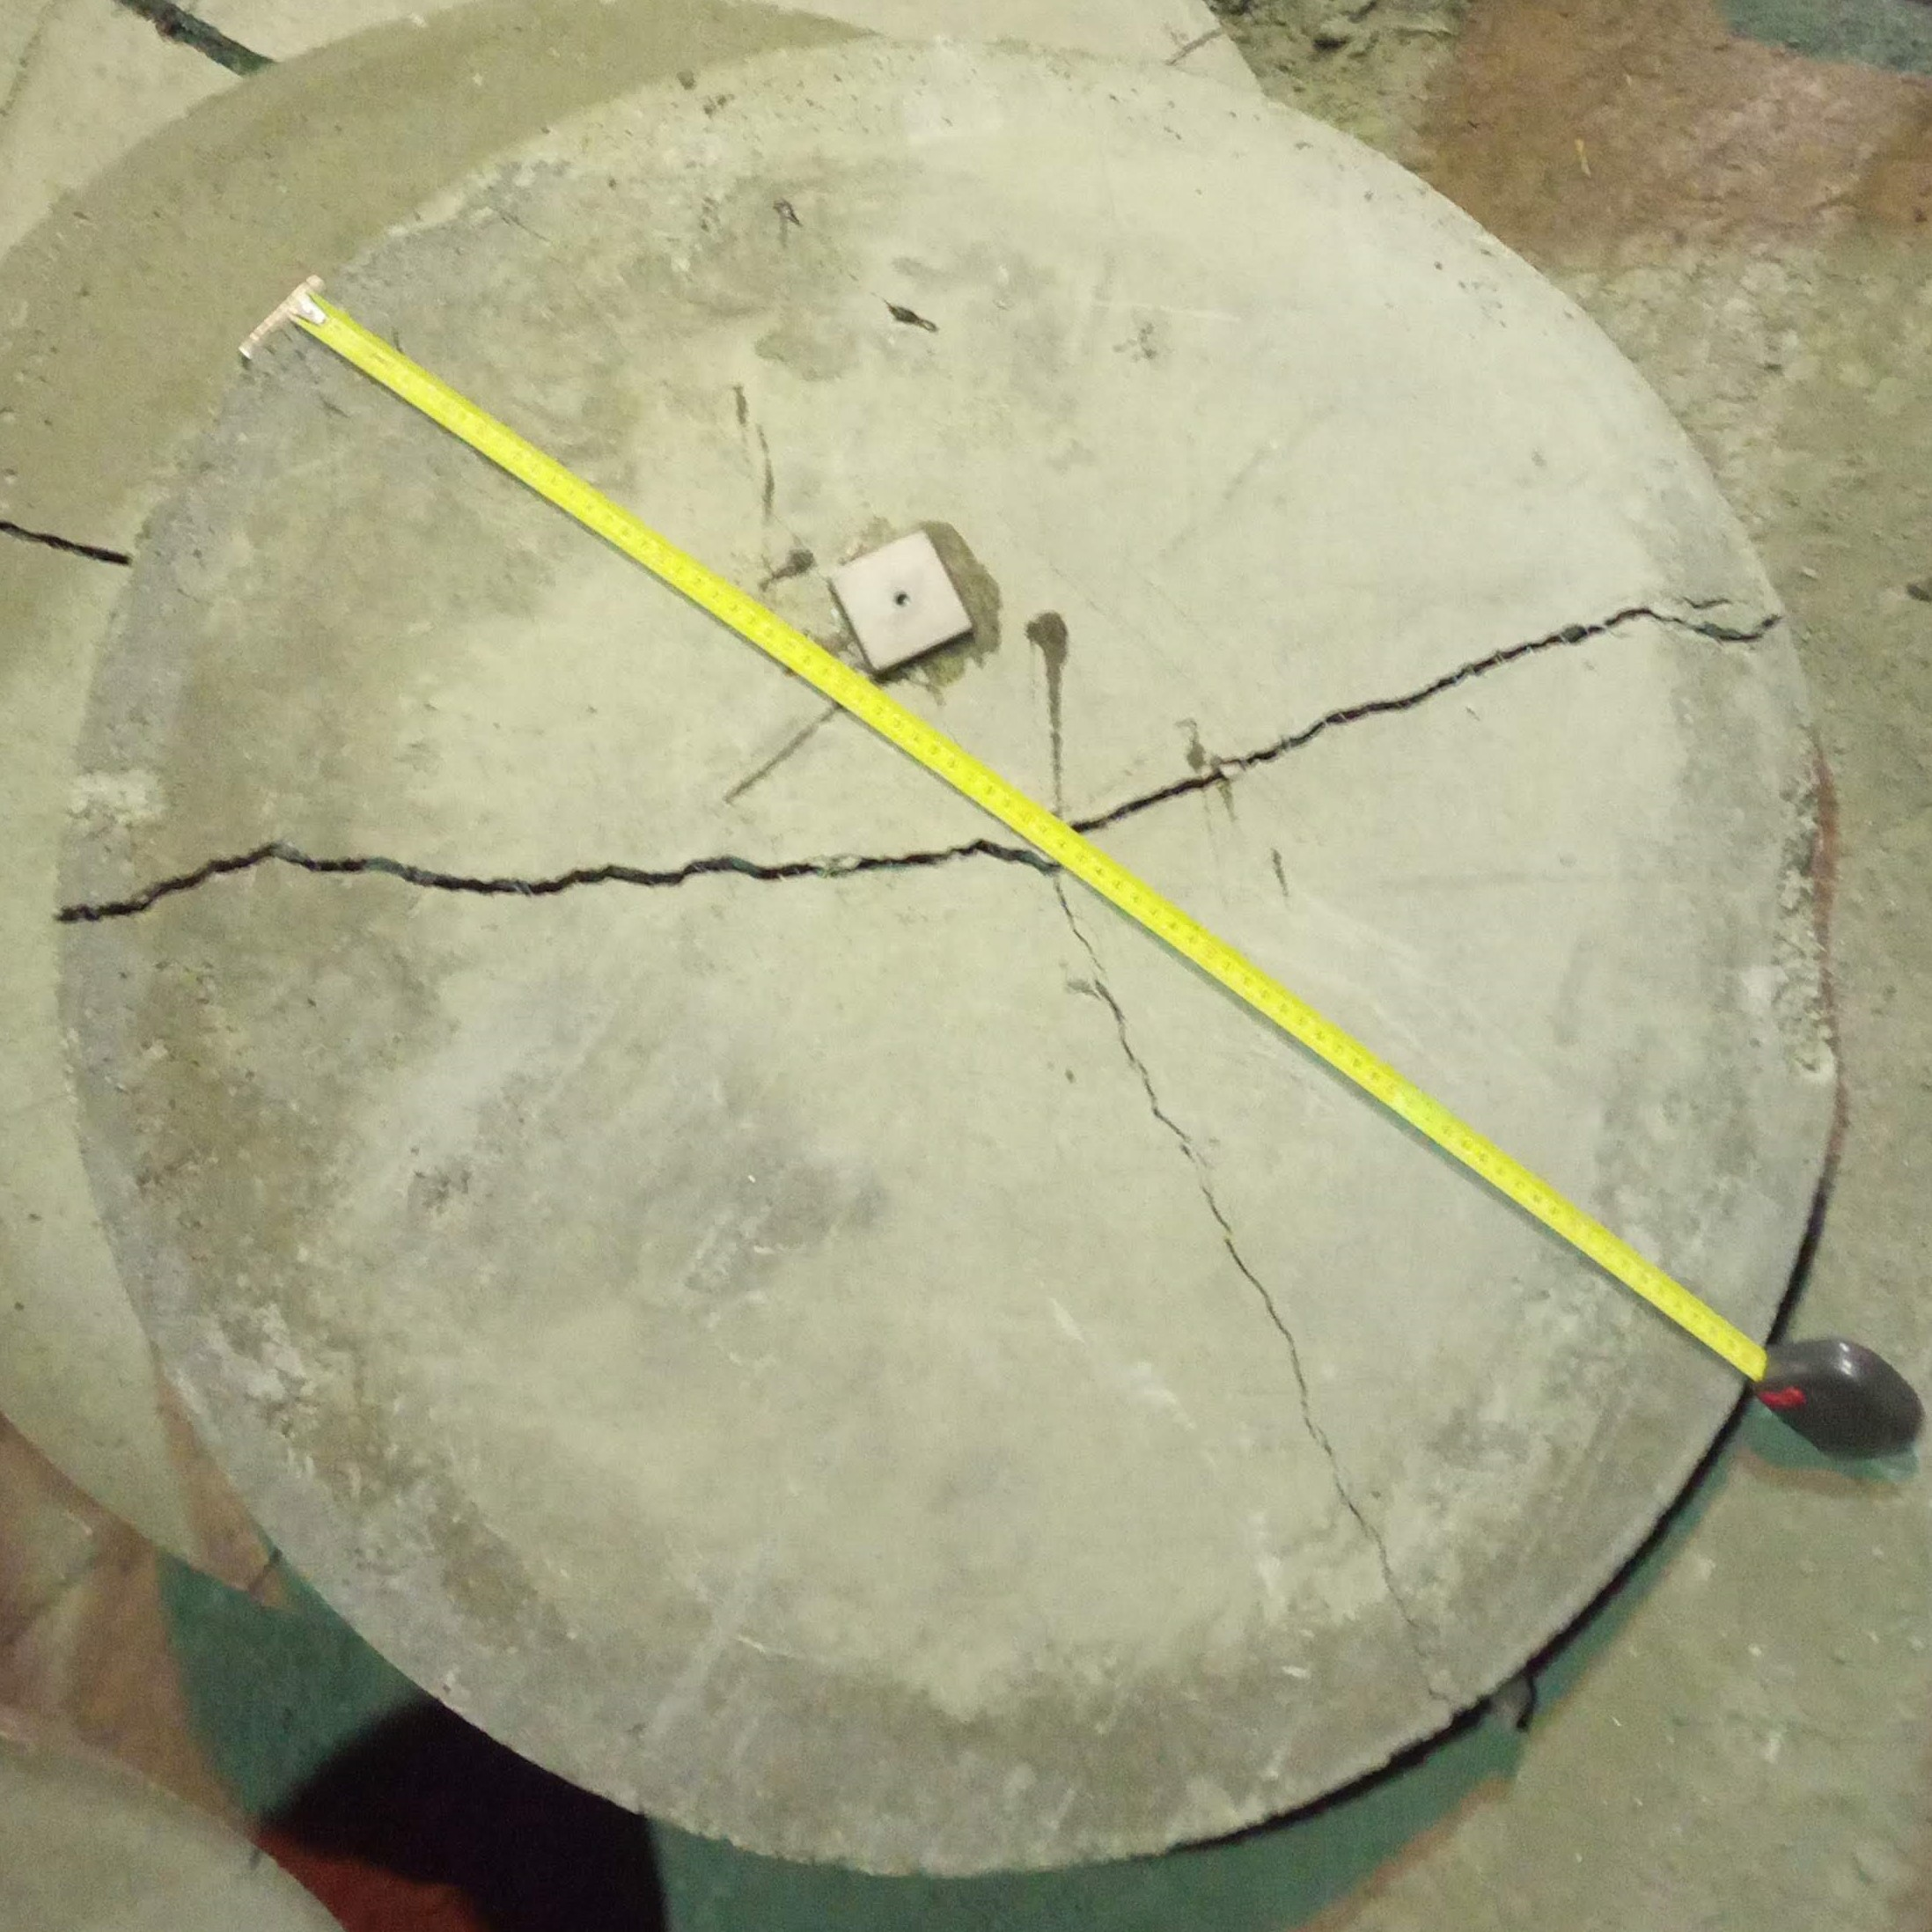
\includegraphics[width = 0.45\linewidth]{appendix/2019-04-16_Rfrs_75_0,5.jpg}}

    \subcaptionbox{sample 2019-05-06\_Rfrs\_75\_0,8}{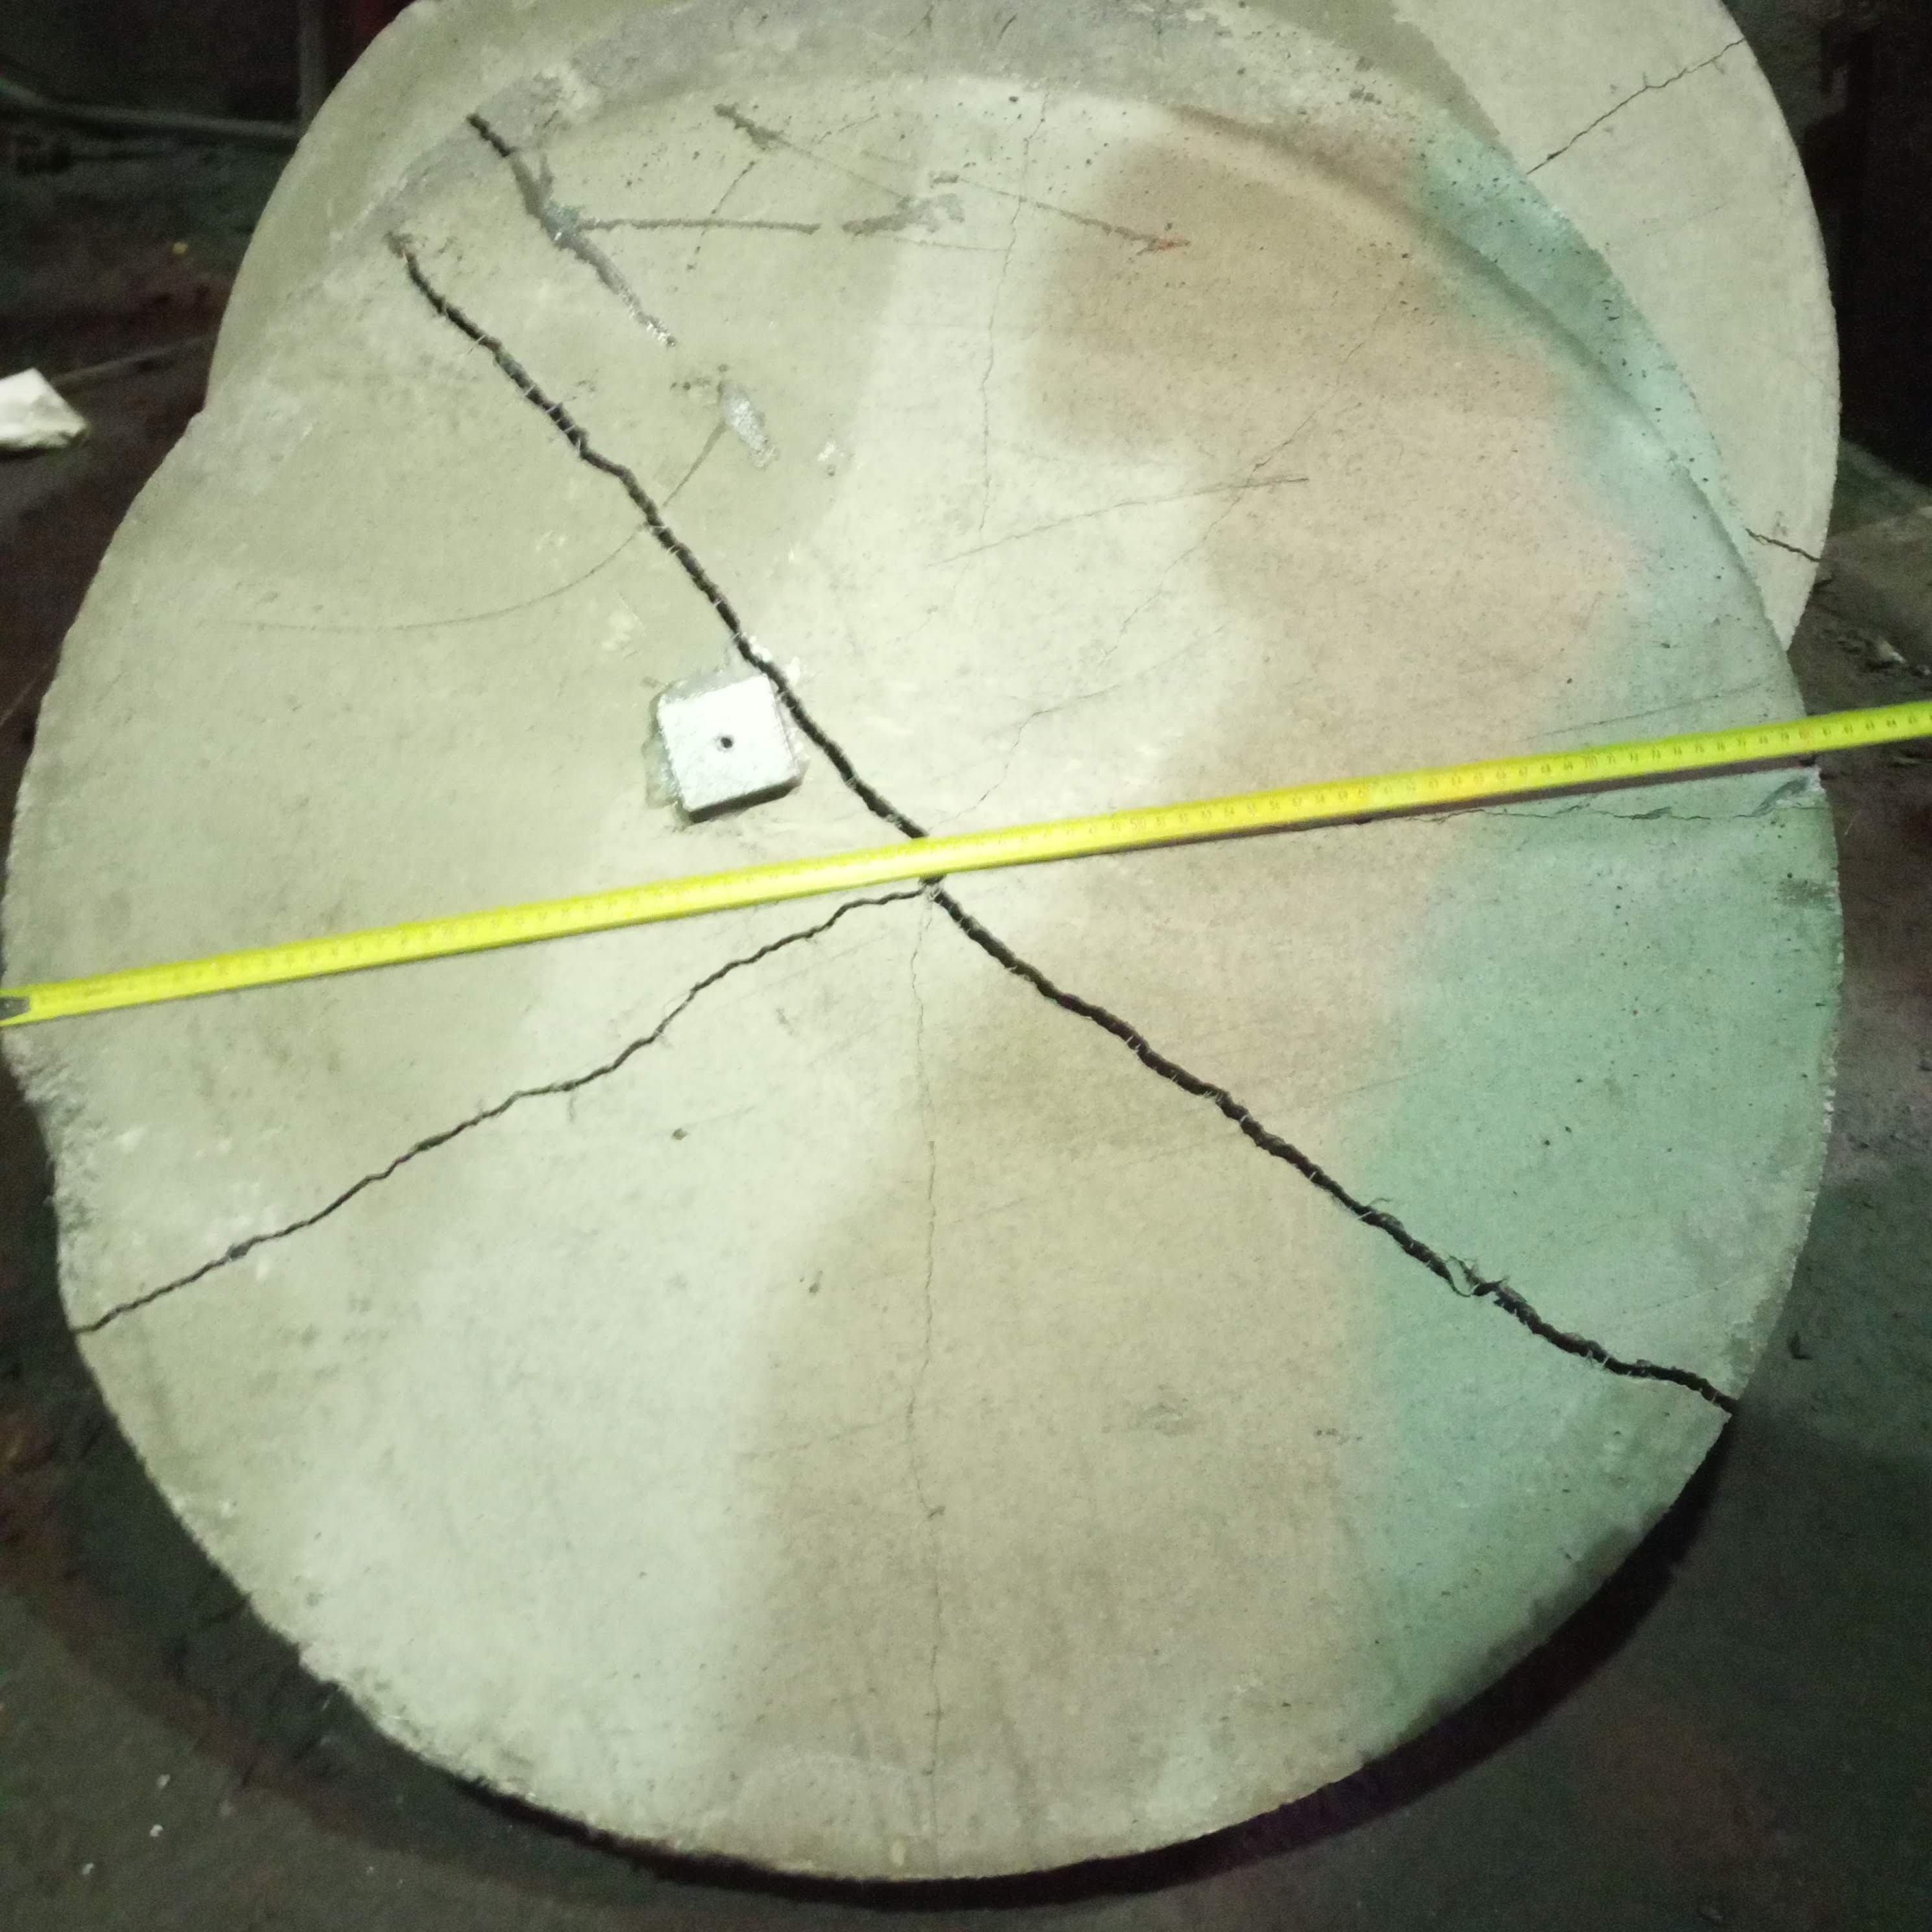
\includegraphics[width = 0.45 \linewidth]{appendix/2019-05-06_Rfrs_75_0,8.jpg}}
    \caption{Crack pattern of samples with additional accelerometers}
    \label{fig:crack_accel}
\end{figure}

\begin{figure}
    \centering
    \begin{tikzpicture}
%sensor array of second campaign under view


%sample
\draw(4,4) circle [radius=4];

%load cells
\draw [fill = blue] (90:3.75) ++ (4,4) circle [radius=.25]
 (210:3.75) ++ (4,4) circle [radius=.25]
 (-30:3.75) ++ (4,4) circle [radius=.25];
\draw (-30:5) ++ (4,4) node (load) {load cell}
(3,6) node [align=center] {expected cracks};

%accelerometers
\draw (4,4) ++ (210:1.5) coordinate (accel);
\draw[rotate=120] (accel) -| ++ (0.25,-0.5) coordinate [pos=0] (that)  -| ++ (-0.5,0.5)  -- cycle;
\draw[fill = red] (4,4) ++ (210:1.25) circle [radius=.1];
\path (4,4) -- ++ (-110:4) coordinate (side);
\draw[rotate=-20] (side) -| ++ (0.25,-.1)  -|  ++ (-0.5,0.1) -- cycle;
\draw[rotate=-20, fill=red] (side) ++ (0.1,-0.1) -- ++ (0,-.2) arc (0:-180:0.1) coordinate [pos=0.7] (here) -- ++ (0,.2);
\draw (0,-1) node (this) {accelerometer};
\draw [-{Latex[length=3mm, width=1mm]}] (this) -- (that);
\draw [-{Latex[length=3mm, width=1mm]}] (this) -- (here);

%cracks
%\path[clip] (4,4) -- ++ (25:4) arc (25:35:4) -- 
%(4,4) -- ++ (145:4) arc (145:155:4) -- 
%(4,4) -- ++ (265:4) arc (265:275:4) -- cycle;

%\path[clip] (4,4) -| ++ (0.2,-5) -| ++ (-0.4,5) -- (4,4) -- ++ (-60:0.2) -- ++ (30:5) -- ++ (120:0.4) -- ++ (-150:5) -- (4,4) -- ++ (60:0.2) -- ++ (150:5) -- ++ (240:0.4) -- ++ (330:5) --cycle;

%\path[fill = lightgray] (4,4) circle [radius = 0.23];
\begin{scope}


\path[clip] (4,4) -| ++ (0.2,-5) -| ++ (-0.4,5) -- cycle
(4,4) -- ++ (-60:0.2) -- ++ (30:5) -- ++ (120:0.4) -- ++ (-150:5) -- cycle 
(4,4) -- ++ (60:0.2) -- ++ (150:5) -- ++ (240:0.4) -- ++ (330:5) --cycle;


\draw [fill=lightgray] (4,4) circle [radius=4];
\end{scope}
\draw[fill=red] (3.5,3.5) rectangle (4.5,4.5);
\draw
(4,5) node {tape};

\end{tikzpicture}
    \caption{Expect crack pattern relative to position of additional accelerometers and loadcells}
    \label{fig:senunder}
\end{figure}

It is possible that the metal plates for the additional accelerometers affected the formation of cracks. When studying \autoref{fig:crack_accel} it becomes obvious that there is one large crack almost straight through the sample. In two cases it went between the two accelerometers. This failure mode was not expected. The samples were supposed to have 3 similarly large cracks with the accelerometer approximately in the middle between two of them, see \autoref{fig:senunder}, the expected failure pattern is shaded in gray. These areas are the ones under tension when the panel is loaded and \autocite{c1550} describes this as the typical failure pattern. 

It was also observed that the samples with additional accelerometers broke at lower energy levels. There are 11 samples with a thickness of 75 mm. Additional accelerometers were used on 5 of them. Without additional accelerometers no sample broke below a 1 kJ impact. The highest impact survived by a sample with additional accelerometers was 0,74 kJ, two samples broke at 1 kJ. Together with the marked change in crack pattern the accelerometers appear to weaken the samples.


\subsection{Load - Displacement Curves}

\begin{figure}
    \centering
    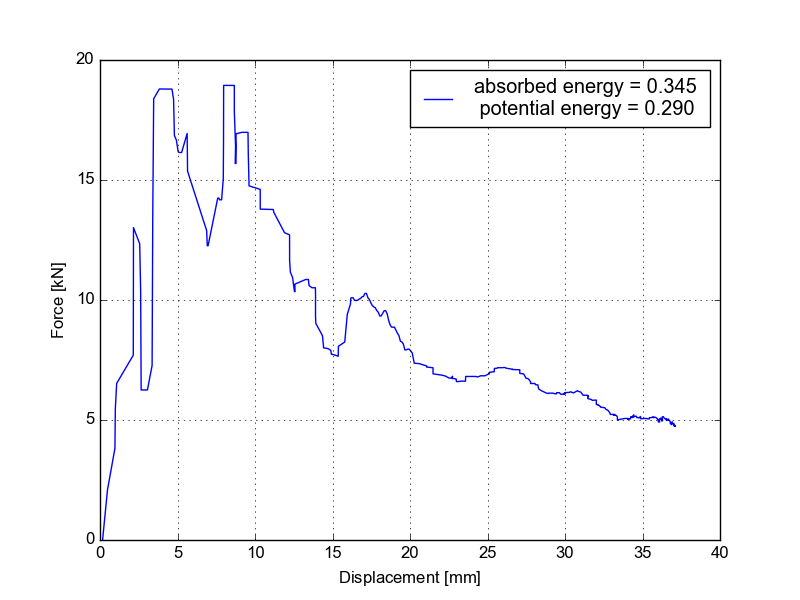
\includegraphics[width=0.95 \linewidth]{pics/2018-12-04_Rfrs_50_0,3_2_energy.png}
    \caption{Energy absorbed during test 2018-12-04\_Rfrs\_50\_0,3\_2}
    \label{fig:energy1}
\end{figure}

\begin{figure}
    \centering
    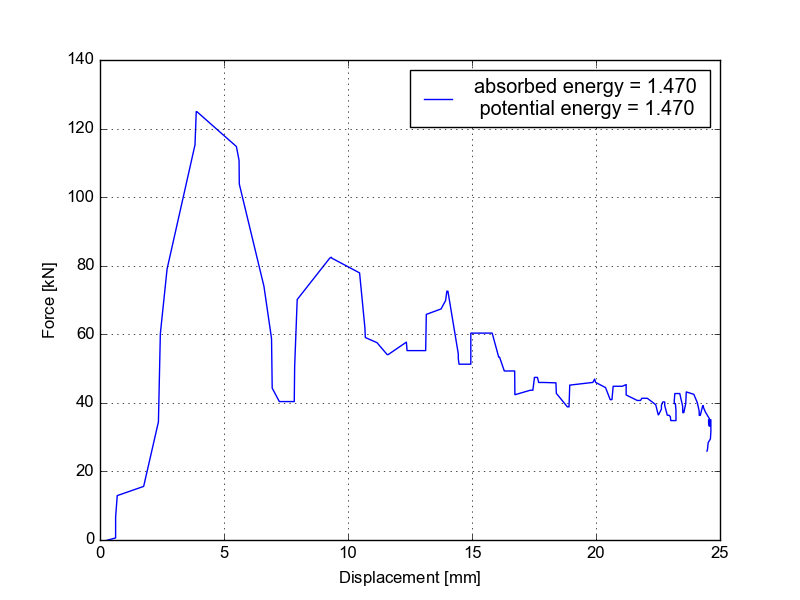
\includegraphics[width=0.95 \linewidth]{pics/2018-12-10_Rfrs_100_1,5_energy.png}
    \caption{Energy absorbed during test 2018-12-10\_Rfrs\_100\_1,5}
    \label{fig:energy2}
\end{figure}

\begin{figure}
    \centering
    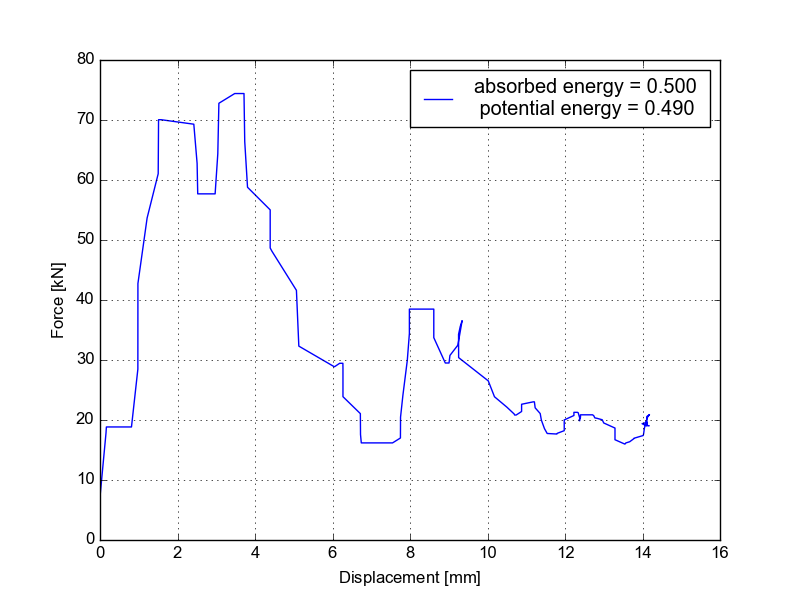
\includegraphics[width = 0.95\linewidth]{pics/2019-02-20_Rfrs_75_0,5_energy.png}
    \caption{Energy absorbed during test 2019-02-20\_Rfs\_100\_0,5}
    \label{fig:energy3}
\end{figure}

\begin{figure}
    \centering
    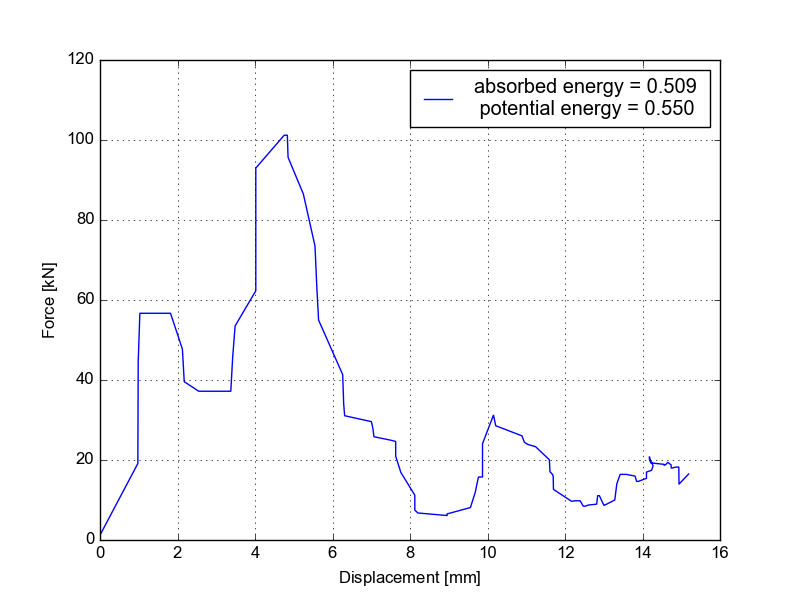
\includegraphics[width=0.95 \linewidth]{pics/2019-04-16_Rfrs_75_0,5_energy.png}
    \caption{Energy absorbed during test 2019-04-16\_Rfrs\_75\_0,5}
    \label{fig:energy4}
\end{figure}

\begin{figure}
    \centering
    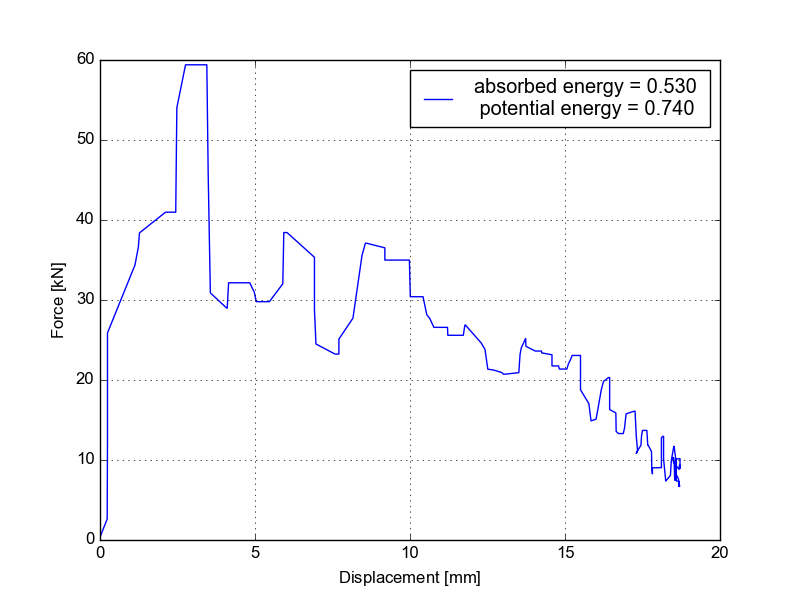
\includegraphics[width=0.95 \linewidth]{pics/2019-05-06_Rfrs_75_0,8_energy.png}
    \caption{Energy absorbed during test 2019-05-06\_Rfrs\_75\_0,8}
    \label{fig:energy5}
\end{figure}

The energy levels used in the analysis of the experiments are the calculated potential energy.
Of course it would be more accurate to calculated the absorbed energy through the load/displacement curve.
As the laser sensor readings were a bit erratic before the tape was applied drawing load/displacement curves and analysing the amount of absorbed energy is only possible for a few tests. 
See \autoref{fig:energy1}, \autoref{fig:energy2}, \autoref{fig:energy3}, \autoref{fig:energy4} and \autoref{fig:energy5}. 
The displacement measurement and the load measurements were synchronised to start at the same time. The initial dip in load was discarded to not interfere with the measurement. 
Some of the displacement curves were cleaned up significantly to be usable. 
The displacement has two parts: the elastic peak deformations and the plastic post peak deformations. 
The curves were drawn until the maximum deformation was reached. 
For two samples the energy absorbed that way was higher or equal to the the potential energy of the drop weight. 
This is of course impossible. 
Energy is dissipated through friction, bouncing, crushing and other factors. 
Therefore the energy measured by the load displacement curves should be lower than the potential energy. 
Some of the energy calculated from the load displacement curves would be released again if the curves had been drawn until the sample deformations had stabilised. 
For the sample 2018-12-04\_Rfrs\_50\_0,3\_2 the very large deformations led to a excessive large energy absorption capacity. It is not clear how the samples managed to derform so much.
For sample 2019-05-06\_Rfrs\_75\_0,8 a lot less energy was absorbed than the drop weight had. It is not clear what caused this discrepancy. There is a strong fluctuation in the displacement curve.
See appendix.
It is not easy to draw load displacement curves with the current sensor data and the energy derived from load displacement curves appears to be questionable at best.
When considering all load curves, see appendix, it is obvious that the thicker panels transfer the force much more quickly than the thinner panels

Overall it seems like using the potential energy to estimate the impact energy is good enough for the round panels. But how are the other parameters affected by the impact energy?



%%%%%%%%%%%%% LINEAR REGRESSION
\subsection{Linear Regression}
\label{ssec:linear}

The results of all tests are summarized in \autoref{tab:leg}. Each test is assigned a number to make them more easily accessible in the following figures. In the text samples will be referred to by (\textit{Number}) \textit{Name}. 
For example: (1) 2017-12-20\_Rfrs\_75\_1,8. The samples were numbered in the order they were tested in.
In \autoref{fig:heat} the coefficient of determination (\(R^2\)) of each parameter pair is displayed in a heat map. \(R^2\) is the normalized mean squared distance of each data point to the linear regression curve. \(R^2\) is a value between 1 and 0. \(R^2~=~1\) signifies perfect linear correlation, with all data points forming a perfect line.
\(R^2~=~0\) signifies a random distribution.
Values that correlate well are dark. Values that do not correlate are light.

\begin{figure}[h]
    \centering
    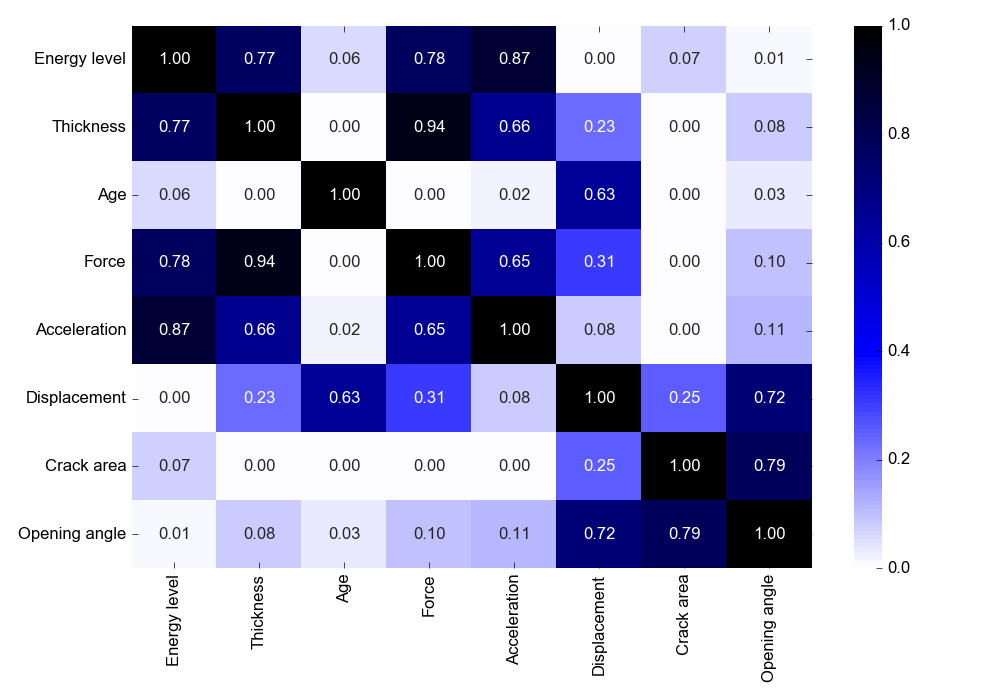
\includegraphics[width = 0.95\linewidth]{diagram/heatmap.png}
    \caption{Heat map of the correlation of various parameters}
    \label{fig:heat}
\end{figure}

\begin{landscape}
\begin{table}
    \centering
\begin{tabular}{l l l l l l l}
\toprule
Name & Number &   Force & Acceleration & Displacement & Crack area & Opening angle \\
&        &         &              &              &            &               \\
\midrule
2017-12-20\_Rfrs\_75\_1,8       &      1 &    3.24 &       278.03 &         -376 &            &               \\
2017-12-20\_Rfrs\_75\_3,5       &      2 &    2.22 &       765.97 &       -168.7 &            &               \\
2018-02-14\_Rfrs\_75\_1,0       &      3 &   75.32 &      1550.01 &         -0.3 &     25.000 &          17.1 \\
2018-02-14\_Rfrs\_75\_0,5       &      4 &   81.38 &      1119.83 &         -0.3 &      4.200 &           1.9 \\
2018-11-09\_Rfrs\_75\_0,5       &      5 &   60.56 &       504.77 &          0.1 &     16.400 &           9.1 \\
2018-11-29\_Rfrs\_75\_1,0       &      6 &   66.97 &      2482.96 &         12.1 &      8.360 &           1.6 \\
2018-12-04\_Rfrs\_50\_0,7       &      7 &   32.31 &       286.95 &          0.3 &            &               \\
2018-12-04\_Rfrs\_50\_0,3       &      8 &   16.91 &       267.72 &          0.1 &     12.860 &          10.6 \\
2018-12-04\_Rfrs\_50\_0,3\_2     &      9 &   18.94 &       368.64 &          0.1 &      7.800 &           5.7 \\
2018-12-10\_Rfrs\_100\_2,0      &     10 &   68.51 &      1983.01 &          0.3 &            &               \\
2018-12-10\_Rfrs\_100\_1,5      &     11 &  128.82 &      2365.65 &          0.3 &     13.600 &           4.9 \\
2018-12-10\_Rfrs\_100\_1,5\_2    &     12 &  161.13 &      2583.81 &          0.2 &      9.400 &           3.2 \\
2019-02-20\_Rfrs\_75\_1,0       &     13 &   70.21 &       1335.8 &          0.2 &            &               \\
2019-02-20\_Rfrs\_75\_0,5       &     14 &   75.47 &       857.11 &              &      4.800 &           3.8 \\
2019-04-03\_Rfrs\_75\_1,0       &     15 &   57.22 &       1457.5 &        -42.1 &            &               \\
2019-04-16\_Rfrs\_75\_0,5       &     16 &  107.47 &      3963.18 &          0.1 &      4.400 &           3.8 \\
2019-05-06\_Rfrs\_75\_0,8       &     17 &   59.66 &      1424.72 &          0.2 &      5.332 &           4.1 \\
2019-08-19\_Rfrs+t\_75\_1,0     &     18 &  113.71 &      1079.74 &          0.1 &      1.400 &           0.8 \\
2019-08-19\_Rfrs+t\_75\_1,0m2,0 &     19 &   60.78 &       358.48 &              &            &               \\
\bottomrule
\end{tabular}

\caption{Summary of results}
              \label{tab:leg}
              \end{table}
\end{landscape}



%As the velocity is calculated directly from drop height, these two parameters should correlate perfectly. They do not, the reason is a rounding error. 
The most important value pairs will be discussed in depth. For this purpose the corresponding graphs are drawn. Broken samples are coloured red and cracked samples are coloured blue, samples that were excluded from the analysis for various reasons are colored gray. 
Some outliers are quite extreme and make the important part of the diagram hard to read. To keep the diagrams readable, these extreme outliers had to be removed from some diagrams. So not every diagram contains every data point. The influence of the drop weight is very obvious when considering the sample (16) 2019-04-16\_Rfrs\_75\_0,5. It is always an obvious outlier.

A linear regression was drawn for the cracked samples with a dashed blue line. \(R^2\) is given in the legend. The intersection with the y-Axis (y) and the slope of the curve (x) are also displayed to allow for fast interpolation of data points.

\begin{figure}[p]
    \centering
    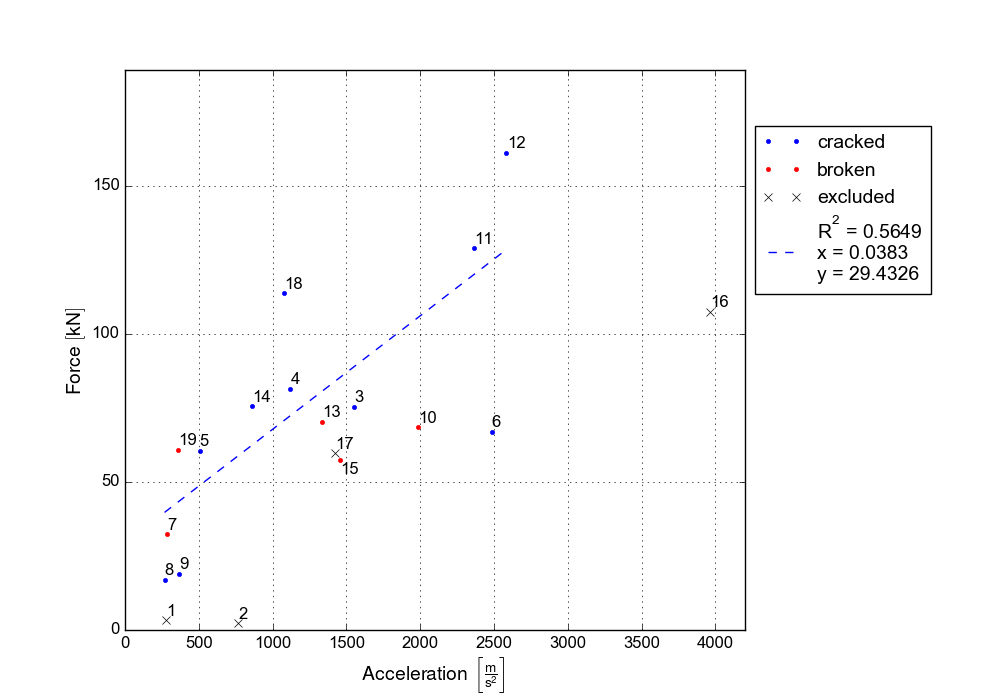
\includegraphics[width=0.95 \linewidth]{./diagram/Force_Acceleration}
    \caption{Force over acceleration}
    \label{fig:Acceleration_Force}
\end{figure}

\begin{figure}[p]
    \centering
    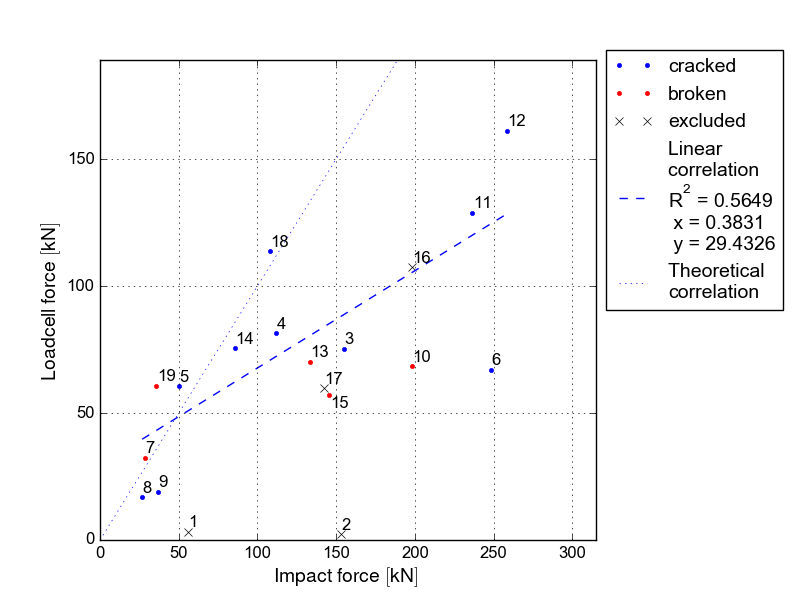
\includegraphics[width=0.95 \linewidth]{diagram/compare_impact_loadcell_force.png}
    \caption{Comparing the force of the impact to the force measured by the loadcells}
    \label{fig:compare_force}
\end{figure}

Force and acceleration correlate well. See \autoref{fig:Acceleration_Force}. Here broken and cracked samples both are very close to the curve. (10) 2018-11-29\_Rfrs\_75\_1,0 is the most obvious outlier because of the high acceleration. 
It was expected that force and acceleration would correlate slightly differently. The force of the impact of the drop weight can be calculated by multiplying the peak acceleration with the weight of the drop weight. According to basic physics: \(F = m * a\).  
As most test were conducted with the 100 kg drop weight the difference between drawing the impact force over the loadcell force and drawing the acceleration over the loadcell force is very small. See \autoref{fig:compare_force} and \autoref{fig:Acceleration_Force}.

Quite noticeable is that (16) 2019-04-16\_Rfrs\_75\_0,5 shifts from being an outlier to fitting very well with the other data. This sample was tested using the 50 kg drop weight. When using several different weights it appears that using the impact force instead of the acceleration might increase the comparability of results. More data is be needed to strength this assumption.

Theoretically  the impact force of the drop weight should be equal to the force measured by the loadcells. In \autoref{fig:compare_force} this theoretical line is presented by a blue dotted line.
In most cases the impact force is lower than the than the force measured by the load cells, the corresponding data points are below the line. %The reason is the energy that is dissipated by the formation of cracks. 
A possible short and simplified explanation would be that the sample starts vibrating when after the impact of the drop weight and these vibrations travel as waves through the sample to the load cells. If the sample forms cracks, some energy of the energy of these waves is absorbed. Therefore the waves are dampened by the time they reach the load cells. This model does not explain the samples where the load cells measure a higher force than the accelerometer does. The effect behind this is not yet understood and could be studied further. Examining the sample that are above or close to the line might yield clues. Sample (5) 2018-11-09\_Rfrs\_75\_0,5 is well above the line. The energy of the impact was 0,5 kJ which is below the critical energy. Probably little energy was lost to forming cracks as the sample was not very stressed.
Samples (7) 2018-12-04\_Rfrs\_50\_0,7, (8) 2018-12-04\_Rfrs\_50\_0,3 and (9) 2018-12-04\_Rfrs\_50\_0,3\_2 were all 50 mm thick. As previously noted, the thinner samples take a longer time to transfer the acceleration from the drop weight to the sample. This reduces the peak acceleration and therefore the impact force. This puts these samples closer to the line. The samples with a thickness of 100 mm, (10) 2018-12-10\_Rfrs\_100\_2,0, (11) 2018-12-10\_Rfrs\_100\_1,5	 and (12) 2018-12-10\_Rfrs\_100\_1,5\_2  are at a distance from the theoretical line still within the normal range. It appears that the thickness has limited influence on the acceleration experienced by the sample. See \autoref{fig:Acceleration_Thickness}.
Samples 	(18) 2019-08-19\_Rfrs+t\_75\_1,0 and (19) 2019-08-19\_Rfrs+t\_75\_1,0m2,0  were the sample. After the initial drop it was tested again. The TSL coat on the sample probably affected its behaviour. 
It appears that there is no simple explanation and that this behavior is dependant on several of parameters.


\begin{figure}
    \centering
    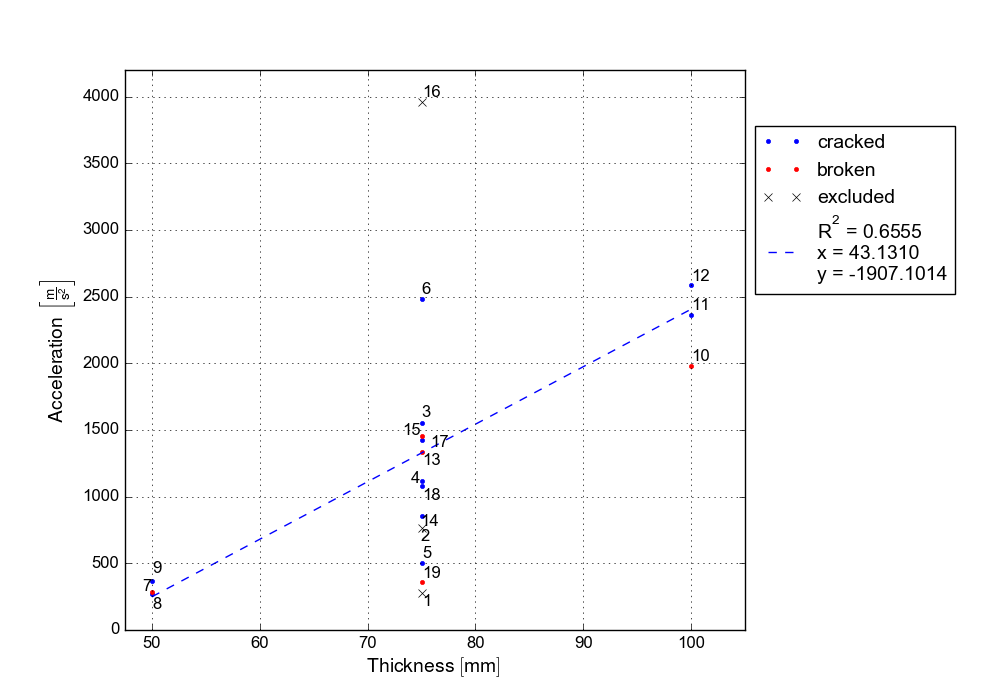
\includegraphics[width=0.95 \linewidth]{./diagram/Acceleration_Thickness}
    \caption{Acceleration over thickness}
    \label{fig:Acceleration_Thickness}
\end{figure}



%The force of the impact of the drop weight can be calculated from the acceleration measured by the accelerometer on the drop weight. 
 

\begin{figure}
    \centering
    \includegraphics[width=0.95 \linewidth]{./diagram/Acceleration_Energy-level}
    \caption{Acceleration over energy levels}
    \label{fig:Acceleration_Energy-level}
\end{figure}

\begin{figure}
    \centering
    \includegraphics[width=0.95 \linewidth]{./diagram/Force_Energy-level}
    \caption{Force over energy level}
    \label{fig:Force_Energy-level}
\end{figure}

The accelerometer on the drop weight and the load cells correlate well with the energy level. See \autoref{fig:Acceleration_Energy-level} and \autoref{fig:Force_Energy-level}. These sensors are both indirect and measure what is going on inside of the sample. In both cases the broken samples mostly fit to the linear interpolated curve.  (4) 2018-12-10\_Rfrs\_100\_2,0 appears to be an outlier. Maybe because of the very high energy level. As long as the sample is not heavily overloaded it does not seem to influence the peak acceleration and the peak force if the sample breaks or cracks.




\begin{figure}
    \centering
    \includegraphics[width=0.95 \linewidth]{./diagram/Energy-level_Thickness}
    \caption{Energy level over thickness}
    \label{fig:Energy-level_Thickness}
\end{figure}

\begin{figure}
    \centering
    \includegraphics[width=0.95 \linewidth]{./diagram/Force_Thickness}
    \caption{Force over thickness}
    \label{fig:Force_Thickness}
\end{figure}

The sample thickness correlates well with the energy level and the acceleration of the drop weight. See \autoref{fig:Acceleration_Thickness} and \autoref{fig:Energy-level_Thickness}. When considering the curves, it seems the linear curve does fit but a poly nominal curve might fit better. There are not enough data points to draw such a curve satisfactorily. The acceleration again seems mostly unaffected by the outcome of the test. Both broken and cracked samples are grouped tightly together.

The thickness correlates extremely well with the force, see \autoref{fig:Force_Thickness}. Most of the broken samples fit quite well with the curve, again (4) 2018-12-10\_Rfrs\_100\_2,0  appears to be an outlier.

\begin{figure}
    \centering
    \includegraphics[width=0.95 \linewidth]{./diagram/Displacement_Opening-angle}
    \caption{Displacement over opening angle}
    \label{fig:Displacement_Opening-angle}
\end{figure}

\begin{figure}
    \centering
    \includegraphics[width=0.95 \linewidth]{./diagram/Displacement_Crack-area}
    \caption{Displacement over crack area}
    \label{fig:Displacement_Crack-area}
\end{figure}

\begin{figure}
    \centering
    \includegraphics[width=0.95 \linewidth]{diagram/Crack-area_Opening-angle.png}
    \caption{Crack area over opening angle}
    \label{fig:Crack-area_Opening-angle}
\end{figure}

\begin{figure}
    \centering
    \includegraphics[width=0.95 \linewidth]{./diagram/Displacement_Age}
    \caption{Displacement over age of concrete}
    \label{fig:Displacement_Age}
\end{figure}

The displacement correlates well with the opening angle of the samples, see \autoref{fig:Displacement_Opening-angle}. Much better than with the crack area, see \autoref{fig:Displacement_Crack-area}. This is somewhat surprising as the opening angle is calculated from the crack area and correlates well with it. See \autoref{fig:Crack-area_Opening-angle}.

The displacement correlates very well with the age of the samples. See \autoref{fig:Displacement_Age}
It is likely that this correlation is just a coincidence due to the small number of data points.
The displacement correlates badly with the thickness of the samples and the peak force. With the energy level and the acceleration it does not correlate at all. This is surprising. It was expected that the amount of damage done to a sample is connected to the impact energy. Perhaps the actual cracking of a sample is more dependant on other factors. For example the crack might start at impurities or micro cracks. It´s outside of the scope of this thesis to make detailed observations of the formations of cracks. In order to be able to make such observations a high speed camera, with a very high frame rate would need to be set up underneath the sample, pointing upwards. At 5000 fps the formation of cracks appears to happen within one frame. A even higher frame rate would be necessary. Pointing the camera upwards at the sample would mean that the camera would have to be protected from debris somehow. Also such observations would face the same problem as the laser sensor readings: debris and dust obscuring the view. It might be worth considering after the impact table has been lifted and more space for equipment is available. 

%The strong correlation between energy level and shotcrete thickness is interesting. If arbitrarily deciding  all parameter pairs with R - values above 0,75 appear to be dependent on each other, the necessary sensor array shrinks significantly. Force and Acceleration both become redundant. Describing both crack area and crack opening angle is also not necessary.

%As long as the drop weight is kept consistent this assumption holds true. As described in %%%%REF 
%had to be removed, as the lighter drop weight changed the measured acceleration significantly. The impact velocity is directly dependent on the drop height.
%The weight of the drop weight appears to have more influence on the response of the sample than the actual energy input. This calls the test setup into question. It is theoretically possible that a sample performs very well when tested using a specific drop weight but poorly under another. Maybe this effect is less pronounced when testing large samples because the load will be distributed by a foam cushion.

%More tests with several drop tests are recommended to study this phenomenon. Perhaps it would be interesting to control the impact velocity.
%When controlling for drop weight the testing process can be streamlined significantly.

As long as the drop weight is held consistent many sensors correlate very strongly.

%%%%%%%%%%%%%%%%%%%%%%%%%%%%%%%%%%%%%%%%%%%%%%%%%%%%%%%%


\subsection{Streamlining the Testing Process}

A very aggressive approach to stream lining the testing process would be to cut the sensor array significantly. As shown in \autoref{fig:heat} all indirect sensors (loadcells, accelerometer on the drop weight and the drop height) correlate extremely well and the direct measurements (displacement and crack pattern) correlate only with each other. The displacement and other ways of mapping the damage of the sample appear to no correlate with the impact energy.

Therefore removing all sensors but the rotary encoder would be a way to reduce both preparatory work and post processing. The drop height is sufficient to estimate of the impact velocity, the force and the acceleration of the drop weight with an \(R^2\) value of > 0,70.

The high speed camera footage is aesthetically pleasing. But data collection is very failure prone, as became obvious when running the experiments. If it does work it is time intensive to evaluate. The results it yields are not very exact, as discussed previously. Therefore it appears redundant.

The accelerometers on the sample are also very vulnerable to failure and require a lot of preparation. They appear to influence the behaviour of the sample significantly. Either a different way of attaching them would be needed or they should be removed.

Tthe malfunctions of both the high speed camera and the accelerometers on the sample were both mostly caused by human error. A check list was implemented to help with this. Further measures to reduce human error would be to synchronise the accelerometers on the sample and the high speed camera with the data collection system. The question that poses itself is, if the data is worth the associated cost.

It was good to test with the full sensor array. Now there is data available that backs up the decision to reduce the sensor array.

When removing all the before mentioned sensors only two parameters still remain to be analysed. The drop height and the thickness of the panel.

\subsection{Correlation Between Thickness and Energy Absorption Capacity}
\label{ssec:energy}

When controlling for the drop weight, the survivable impact energy and the thickness of the panel appear to be linearly dependant. The parameters necessary to estimate the thickness at which a sample is sure to survive at a certain energy input are given in \autoref{fig:Energy-level_Thickness}. They can be summarised in a equation to enhance understanding. The round panels have a surface area of approximately 0,5 m. These equations are using rounded factor and have been modified to work per square meter of concrete.

See \autoref{equ:energy}.

%The slope is \(32,6203~\frac{\text{mm}}{\text{kJ}}\)  and the intercept is \(50,5644\) mm.  

\begin{equation}\label{equ:energy}
    \text{Necessary concrete thickness [mm]} = 16,5 ~\frac{\text{mm}}{\text{kJ}} * \text{Energy input [kJ]} + 25 ~\text{mm}
\end{equation}

 Through simple arithmetic the reverse equation can be deduced. See \autoref{equ:thickness}

\begin{equation} \label{equ:thickness}
    \text{Survivable energy [kJ]} = 0,047 ~\frac{\text{kJ}}{\text{mm}} * \text{Sample thickness [mm]} - 2,02 ~\text{kJ}
\end{equation}

The limitations of these equations are quite strict. They only apply for the type of concrete used in Kirunavaara mine with a thickness between 50 and 100 mm, when using a 100 kg as drop weight and using round panels. It should be mentioned that this is the linear interpolation of all samples that only cracked. Some samples broke at lower energy levels and some samples survived higher impacts.

\begin{table}
    \centering
    \begin{tabular}{ll}
    \toprule
    Thickness [mm]  & Energy [kJ]\\
    \midrule
    50             &   0,3 \\
    60              &   0,8 \\
    70             &   1,3 \\
    80              &   1,7 \\
    90             &   2,2 \\
    100              &   2,7 \\
    \bottomrule
    \end{tabular}
    \caption{Concrete thickness necessary to survive certain impact energy}
    \label{tab:estimate}
\end{table}

Using these equations it is possible to estimate the thickness of shotcrete required to survive various impacts. See \autoref{tab:estimate}. The current shotcrete thickness is 100 mm. This appears to be able to survive impact energies of 2,7 \(\frac{\text{kJ}}{\text{m}^\text{2}}\). %\textcite{Heal10} stated that FRS without mesh support fails at 1,5 to 2 \(\frac{\text{kJ}}{\text{m}^\text{2}}\) \textit{in - situ}.

%This design load appears to be significantly too high. 
Large sample tests are recommended to confirm these equations. \textcite{Potvin10} stated that 100 mm of FRS in drop tests usually achieve energy absorption capacities of between 5 - 10 \(\frac{\text{kJ}}{\text{m}^\text{2}}\). 
The results of the Kirunavaara test rig using round samples are significantly are lower than those of other test rigs. This should be taken into consideration when comparing results with other test rigs. A reason might be the shape of the drop weight.

\chapter{Next Steps}

%In this chapter I will describe the best possible support elements in detail and will elaborate on their weaknesses and strengths and what further tests should be done to confirm my findings.
%As well as possible alterations to the rig in order to conduct further tests.

Drop tests can only judge the mechanical properties of support components. When designing a support system other factors are also at play. The usability of a support component is not just dependent on its mechanical properties such as energy absorption capacity or displacement capacity. Economical factors are also at play.
The potential to mechanise or automate the installation is an important factor when considering the usability of a support element. Especially in countries with high labor cost, such as Sweden.
The longevity of a component should match the lifespan of the excavation it's supporting. Excessive moisture and acid mine drainage can destroy support elements prematurely. \autocite[2]{player04} \autocite[8]{Simser07} Corrosion plays a part in bolt failures during rock falls. \autocite[8]{villa13} When following up with the research done in this thesis such factors will have to be taken into account. 

The testing method has not been exhaustively optimised. The drop test rig in its current form still has a lot of untapped potential. For example the sensor array could still be improved.
%There are a lot of possible chances to enhance the rig. In its current state only a fraction of its potential is realized.


\section{High Speed Camera}
%A better highspeed camera than the Casio Exilim Pro Ex-F1 might 
The high speed camera footage allows for visual inspection of the data and provides a secondary way to measure displacement. %As of yet no tests have been run using the Phantom Miro LC110 therefore no comment can be made on how it improves the test results. 
So far the high speed camera is very failure prone. By integrating it in the data logger some handling mistakes could be avoided. Then the measurements could also be synchronized. 
Measurements could also be synchronized without integration. For example by turning on an LED at known point in time.

The high speed camera needs high ambient light for best results. Sourcing this light can be difficult. LEDs are known to flicker but at the frame rates that were used so far (up to 5000 fps) this did not impact the quality of the measurements.
Finding enough power outlets is another problem. The test rig only has 5 electrical outlets and when deploying a high speed camera with corresponding laptop needed to control it and several light sources this amount of outlets is insufficient. The resulting amount of drawn power triggered the breakers several times during testing.

\section{Laser Sensor}

%The laser sensor works by measuring the change in the intensity of the laser beam. When the object that the laser is pointed at moves towards the laser the light intensity increases. When the ambient light is bright enough the sensor does not register this change anymore. Therefore low ambient light is favorable when using a laser sensor. Using both high speed camera and laser sensor at the same time would require a compromise in both of their effectiveness. Or a conscious choice for one over the other. The laser sensor is more precise and allows drawing of load displacement curves but it is much more failure prone than the high speed camera. The high speed camera creates visually pleasing videos that can be used for qualitative analysis and representative purposes.

The laser sensor is sensitive to dust or debris falling through the laser beam. Applying the reflective tape to the sample appears to have increased the usability. Still some post processing is required to draw load displacement graphs. Maybe with a different sensor even the need for this could be removed and the data processing could be automated entirely. It would then only require an operator to run the tests and an engineer to look over the graphs. %Especially since the laser sensor and the high speed camera do not work well together. The laser sensor requires low ambient light.

%does not provide reliable data and therefore can not be used in a meaningful way. Therefore our top priority should be to find an alternate way of measuring displacement. Perhaps with an ultrasound sensor, LED sensor or inductive sensors. 

\section{Measuring Velocity}

It would be cautious to measure the impact velocity of the weight somehow in order to confirm the calculated values. Perhaps using two light gates or a line reading camera. Either the variation of impact velocity used in the tests should be minimized or the effects of different velocities would have to be studied. \autocite[25]{Erik15} specifically talks about punching. A failure mode that occurs at high impact velocity, where sample get concentrical cracks in addition to the usual radial ones.

%It would make sense to synchronize the high speed camera with the sensor measurements somehow. Either through integration in the data logger or an LED switching on at a known point in time. It might also be worthwhile considering to trigger the camera together with the other equipment. Currently the highspeed camera has to be triggered manually, which is very failure prone and has already lead to the loss of data from one test.%Also a different camera would probably have to be triggered remotely just before the impact, because of limited data storage capacity.

\section{Load Cells}

Currently the load cells are located at the corners of the concrete slab which imposed the static load. There is no real world equivalent for this force. As such it would make more sense to instead have load cells at the bolt points, to capture the stresses which would be inflicted on the bolts in the given scenario. Such load cells exist and are called force rings.

\section{Drop Weight}

To ascertain the influence the weight pf the drop weight has on the outcome of a test all drop weight should be tested. One option would be to try every drop weight at the same energy level and then at the same impact speed. 
Like this the influence of the impact speed could be determined.

\section{Direct Sensors}

More direct sensors would reveal more about how the sample behaves under load. But these sensors can influence the result positively or negatively. In case of the additional accelerometers the influence was obviously negative. The reasons would need more investigation. The use of the current system is discouraged. The accelerometers could alternatively be screwed directly into the sample.

\section{Testing Surface Support}
\label{sec:mesh}

In the current setup there is very little space for displacement. Too little for the testing of mesh, especially chain-link or textile mesh, which are known for their capacity to deform heavily. Lifting the impact table should be considered in order to increase the testability of different mesh types. Additionally to mesh, different types of straps or lacing should be tested as well. The only type of strap currently in use at Kiirunavaara mine is called %Fjällband, which is currently only used in a very specific use case, will also be tested.
 Fjällband. It is currently only applied laterally between crosscuts in order to  hold the pillars together. %This usecase is generally refered to as a "bull nose". 
 %Fjällband might have a lot of potential or could be entirely cosmetic but there is simply no possible way to know it is tested. 
 There is very little to no documentation on Fjällband so additional tests such as pull strength or shear strength tests, are advisable. Also it might give interesting results to test Fjällband not just singly but also crossed. It has never been applied in such a fashion in the mine but there might be a positive effect.

%There are plans to test lacing. But only one type of steel rope. 
Lacing is a very undefined concept. There are no defined diameters or rope types. Therefore it would make sense to test a lot of different ropes. Lacing is usually steel rope. Synthetic rope could prove to be and interesting alternative.
%Maybe synthetic rope could be an interesting alternative.

%In order to be able to test lacing as well a contraption to attach lacing cables to the frame will be build. 
\section{Sample Preparation and Post Processing}

%Sample preparation is a very important factor. %A quick fix might seem attractive but will carry a host of difficulties. It might make more sense to make a more complicated modification now, that requires less work in sample production later. 

There are four key attributes a test can have.
It can be realistic or abstract, lean or extensive.

Realistic means that the testing conditions are as close to the \textit{in - situ} conditions as possible. %This means that the test has low repeatability, needs more preparation than a more abstract test and is more cost and time intensive.

Abstract tests take the \textit{in - situ} conditions and try to simplify them as far as possible and make the result test procedure more repeatable and cheaper. 

Extensive tests try to gather as much data as possible and decide in post-processing what is useless and what is useful. This kind of tests takes a lot of time in preparatory work and in post processing. If there is not much experience with the testing method extensive tests are a good first step. The results can be surprising and entirely unexpected.

Lean tests are reduced to the bare minimum of preparatory work, sensors array and post-processing. This makes them cheap and fast to run. But a lot of decisions have to made beforehand. It is much harder to have unexpected results or discover new things with a lean test. Lean tests work best if there is already experience with the subject matter and the goal of the experiments is very well defined.

Drop tests are more abstract than blast tests. Repeatability, low running cost and high test frequency are their strong suit. The round panel tests are very abstract, the square tests try to be more realistic. The current sensor array is quite extensive and includes a few redundancies. It could be probably be shrunk without decreasing the quality of the analysis. 

%The question poses itself how in-depth the future analysis of results has to be. 

In this thesis it has been proven that the impact velocity and the impact energy can be estimated with good precision using the mass of the drop weight and the drop height. 

For each parameter that is being measured or could be measured the following questions should be asked.

In the best case scenario, what can we learn from measuring this parameter? Is it important to know the exact value? Is an estimation good enough? Does it correlate or depend on other parameters? How would the analysis of test results be influenced if it was neither measured nor estimated?

If the knowledge of a parameter in the best possible scenario is not interesting or relevant it does not make sense to measure it at all. 
Exact values are more expensive than estimations. The price of sensors increases with their precision. Therefore more exact values are more expensive. Precise values require additional time in both preparation and post processing when compared to estimations. If a parameter correlates with or is dependant on other parameters or if it does not influence the analysis of the test results it might redundant and could perhaps be removed. If it has little influence on the analysis of the test results it does not need to be measured redundantly. If a value has a strong influence on the analysis of the test results it should be to measured redundantly. 

%The additional accelerometers require a lot of preparatory work. The metal plates to which they are attached need to be manufactured and can not be reused. The metal plates need to be glued on at least a day in advance so that the glue can harden sufficiently. The data gathered from the additional accelerometers, the built-in sensors and the high speed camera has to be synchronised in post processing. The data from the laser sensor needs to be cleaned up to be usable. All of which requires valuable time. 

%This thesis tries to provide the reader with the knowledge to necessary to decide which of these sensors are redundant and which are vital. %This poses the question: is all this data really necessary?

%The strong point of impact tests is their repeatability, their low running cost and the high volumes of tests that can be run in a short time frame. All of which would suffer greatly from a high overhead as would be imposed by elaborate preparatory work. The additional accelerometers already require additional work. The metal plates to which they are attached need to be manufactured and can according to our current knowledge not be reused. The metal plates need to be glued on at least a day in advance so that the glue can harden sufficiently. The data gathered from these sensors and the high speed camera has to be synchronised in post-processing. The data from the laser sensor needs to be cleaned up to be usable. All of which requires valuable time. This poses the question: is all this data really necessary? %Is it even possible to turn it into information without being overwhelmed? 
Maybe it would be easier to just find a quick way of measuring post peak capabilities of the system and then present those together with the energy level of the impact and ignoring all the other values. It´s simply a question if running a few very well monitored tests or a lot of simpler tests with a leaner sensor array is preferable. The round sample tests are easier to conduct than the large sample tests and round samples can be produced quicker and are cheaper. Maybe a two step system would be best. First round sample tests could be run with little instrumentation and used for pre-selection. The remaining sample types could then tested in a larger scale with more instrumentation and more careful analysis. Before having such considerations about the testing paradigm it might be worth considering what could be changed about the samples.

\begin{comment}
%Outer confinement changes the behaviour of mesh significantly. Therefore it might be interesting to be able to confine ductile materials such as mesh with varying stiffness or not at all edges.
\begin{figure}
    \centering
    \begin{tikzpicture}
%top view clover leaf mesh

%draw the clip path
\path[clip, draw] (1,0) -- (1,1) -- 
(0,1) -- (0,4) -- (1,4) -- 
(1,5) -- (4,5) -- (4,4) -- (5,4) 
-- (5,1) -- (4,1) -- (4,0) --cycle ;

%draw the mesh
\draw [help lines, step = .1cm] (0,0) grid (6,6);



\end{tikzpicture}
    \caption{Necessary shape of mesh to create the right boundary conditions} 
    \label{fig:meshBound}
\end{figure}
\end{comment}
\begin{comment}
\begin{figure}
    \centering
    
    \subcaptionbox{Sideview of a possible way to produce stiff boundary conditions \label{fig:sideBound}}{
    \begin{tikzpicture}
%TOP VIEW OF MESH BOUNDARY

%concrete slab
\filldraw[fill=lightgray] (0,0) rectangle (6,2)
node[pos=.5] {concrete slab};

%sample
\filldraw[fill=gray] (0.5,0) rectangle (5.5,-0.5)
node[pos=.5] {specimen};

%mesh
\draw[thick,rounded corners = 8pt, dashed] (-0.2,2) -- (-0.2,-0.7) -- (6.2,-0.7) node [midway, below] {mesh} -- (6.2,2);

% bolts
\draw[thick]
(1.5,2.3) -- (1.5,-1)
coordinate [pos=0.05] (bolt1)
(4.5,2.3) -- (4.5,-1)
coordinate [pos=0.05] (bolt2);

%sidebolts
\draw[thick] (-0.5,1.5) -- (1,1.5)
coordinate [pos = 0.5] (sbolt1)
(5,1.5) -- (6.5,1.5)
coordinate [pos = 0.5] (sbolt2);

%BOLTS
\draw (3,3) node (bolts) {bolts}
[->] (bolts) .. controls ++ (-0.5,-0.75) .. (bolt1);
\draw [->] (bolts) .. controls ++ (0.5,-0.75) .. (bolt2);

%SIDEBOLTS
\draw (3,4) node (sbolts) {sidebolts}
[->] (sbolts) .. controls ++ (-2,0) .. (sbolt1);
\draw [->] (sbolts) .. controls ++ (2,0) .. (sbolt2);



%what else do I want in here??
%the side bolts
%maybe a sketch of the loom
%pretty graphics anyway

\end{tikzpicture}
    }
    \subcaptionbox{Necessary shape of mesh for this set up \label{fig:meshBound}}
    {
    \begin{tikzpicture}
%top view clover leaf mesh

%draw the clip path
\path[clip, draw] (1,0) -- (1,1) -- 
(0,1) -- (0,4) -- (1,4) -- 
(1,5) -- (4,5) -- (4,4) -- (5,4) 
-- (5,1) -- (4,1) -- (4,0) --cycle ;

%draw the mesh
\draw [help lines, step = .1cm] (0,0) grid (6,6);



\end{tikzpicture}
    }

\caption{One possibility of creating stiff boundary conditions}
\label{fig:stiffBound}
\end{figure}

Especially chain-link mesh´s strength lies in its ability to transfer load across a large area which is very hard to replicate. There are a few ideas floating around, some of which are more complicated to manufacture than others. In \autoref{fig:stiffBound} one idea is displayed. In \autoref{fig:sideBound} a side view of the idea is given. The basic principle would be to pull up and attach the mesh to the sides of a concrete slab. Possible ways of attachment would be addition bolts for example. The drawbacks of this method lie in the very difficult sample preparation, firstly the corners would need to be cut from each sample to give it a clover leaf shape as displayed in \autoref{fig:meshBound}.% additionally the "leaves" would have to be bend at a 90 degree angle without breaking any of the wires or welds. Another idea was to built a sort of comb / loom which would not require any bending of the mesh, but this topic will require further discussion in order to solve. 
\end{comment}




%Especially because of the boundary conditions \textit{in - situ}, the the welded mesh panels currently in use have a size of 2,3 on 2,2 m and a bolt spacing of 1 bolts per meter. See \autoref{fig:insituMesh}. Which means that a 1 x 1 m square of mesh has two open boundaries and two flexible boundaries (illustrated in \autoref{fig:insituMesh} with red dashed lines). At least welded mesh panels should be tested in such a way, that these boundary conditions are properly reflected. Which means that two ends of the mesh should be free and two should be constrained somehow. 
 
\section{Concrete and Shotcrete}

According to the current plan, all specimens made from concrete will be cast instead of sprayed. Therefore they are likely to exhibit better properties than could be expected in the field. Spraying the samples would be additional work but the test results would gain credibility. At least  a few tests should be run with shotcrete in order to give some guidance on the reduction in strength that could be expected if such a specimen production regime had been implemented.

\section{Adhesion Between Sample and Concrete Slab}

All currently planned samples will use the adhesion between sample and concrete block. It might be interesting to see how large this adhesion is and therefore a few sample without it should be tested.

The concrete slab is costs a lot of material, makes the samples much harder to handle and increases the sample production time. The value it adds to the experiments has to be worth this cost. Until this worth is not proven, using the concrete slabs is questionable.

\section{Thickness of the Concrete}

It is hard to judge the effect the thickness of the concrete has on its energy adsorptions capabilities. The force measured by the load cells and the acceleration of the drop weight appear to be independent of the thickness of the sample. Just the deformations (which were problematic to measure in the past) and the crack patterns appear to be affected by the thickness. Maybe the accelerometers attached directly to the sample would be affected as well, but as there were no tests conducted with additional accelerometers and a thickness other than 75 mm it is impossible to say.
%are no more tests planned with a thickness other than 75 mm it will be impossible to find out.

%It might be interesting to look into TSL as an alternative to shotcrete. 

\section{Degree of Destruction}

To quantify to the degree of destruction of the samples after a test the displacement and the size of the resulting cracks was measured. These did not correlate with the energy level at all. It appears that the formation of cracks is much more dependant on the sample composition than on the impact energy. 
Maybe a different way of measuring the destruction of a sample should be considered. The very simple division into the two categories "broken" and "cracked" is not quantitative. 
One way could be conducting a quasi-static test after a dynamic test on the same sample. This way  the post-peak capabilities of the sample could be determined. 

\section{Quasi-Static Test Rig}

In order to understand the properties of the tested samples better it would be interesting to know their static load capabilities. Therefore adding a quasi static test facility to the existing rig might be worthwhile. The most important factor when considering this is the magnitude of the required precision. A basic idea, which is to say a margin of error of a few percent or more, should be sufficient. It seems better to have some idea about this than none whatsoever. If it turns out that the static capabilities are more interesting that previously thought the rig can always be upgraded further. 

As the formation of cracks is quite random, the quasi static capabilities might be too. Therefore knowledge of the static capabilities might add little value to the analysis of the test results. %it does not make sense to waste too many resources on it.

%It might be interesting to not just test the static capabilities alone but to test the static capabilities that remain after an impact test. This would give an idea about the post peak capabilities of the tested surface support.

%\section{Post peak capabilities}

%With the current rig the post peak capabilities are hard to assess. Some thought should be put into how this could be done in a qualitative way. 

\section{Bolt Test Rig}

The current rig cannot tests bolts. It might be interesting to tests bolts both dynamically and statically. Something to consider would be to not just test the tensile strength but to also consider ways to test the shear strength. Often the shear strength of bolts is not considered when designing a support system but it often leads to failure during rockbursts. \autocite[17]{guler01} When the rig has the ability to test bolts it's not a very large step to testing bolts and surface support together as a support system.

\section{Support System}

 It might be very interesting in the future to inspect the interplay of different surface support concepts with different bolts. To achieve this, the threaded bars that serve as bolts would need to be replaced with real bolts. The samples would need to be suspended by the bolts instead of resting on the load cells and instead forces would need to be measured using for example force ring located between bolt plate and concrete.
 
%This list does not claim to be exhaustive but merely a collection of suggestions. With all these possible enhancement and modifications in mind it is crucial to prioritize and focus on what is really important.







\chapter{Discussion}
\label{ch:con}

%Why was it necessary to write this thesis?
%What were the results?
%What are the next steps?
%In brevity.

With increasing depth, stresses inside the rock mass surrounding the stope increase. When these stresses surpass the strength of the rock, it is bound to fail. In case of strong, brittle rock, which shows little ductile behaviour, tensions cannot be reduced through continuous deformations. These tensions build up and can be released explosively. %, rocks might get ejected from the walls and ceiling into the cavity.
Such an event is called a rockburst. They are often connected to seismic events of natural or artificial origin. An example for a seismic event of artificial origin is blasting. As blasting is a regular occurrence in most underground mines and developments in technology allow for economical exploitation of ore bodies located deeper than ever before, rockburst are an extremely relevant topic.

Rockburst occurrence and severity can be reduced through various methods, for example: changing or modifying production sequence, mining geometry, mining method, excavation shape, location of drifts and ore passes, and stope size. These measures can reduce the stress on the rockmass in advance. Destress drill and blasting can be used to actively reduce the likelihood of a rockburst in a limited area. \autocite[219]{Kaiser12}

The last line of defence against rockbursts is rock support. There are two kinds: reinforcement support and structural support. 
Reinforcement support is usually realized through rock bolts. There are several kinds with some being especially designed to take the dynamic loads caused by rockbursts. Reinforcement support aims to increase the strength of the rock mass to the point at which it can support itself. 
Surface support is more varied than reinforcement support: shotcrete (not reinforced, fibre reinforced, mesh reinforced), steel mesh, lacing, straps and combinations of these all function as structural support. Surface support together with reinforcement support forms a safety net that reduces the risk of rock falls by capturing loose rock or securing wedges which would be prone to fall by anchoring them to unbroken rock. As the weakest link of a support system will fail first, a support system must be considered holistically.

Without the danger of rockbursts, such rock support systems are designed to withstand static load. The change in pressure of the rock is slow, resulting in quasi-static loading conditions. In burstprone ground  sudden high energy bursts must be absorbed by the support system as well. %This is usually achieved by allowing deformations, channeling energy into friction or other ways of turning the destructive energy into less harmful effects. 
A system cannot be designed for the sole purpose of absorbing energy. It must also withstand the static load imposed by the surrounding rock mass. \autocite[233, 234]{Heal10} 

Developing fitting rock support systems is difficult as they must be adjusted to local conditions and few practical test methods are available, even fewer of them standardized. Taking data from past rockbursts and gathering data about energy levels of past seismic events, their locations and how the rock support reacted to them is one important source of information. The limitation of this information is, that only the current support system can be evaluated. If a new support system would be tested this way it would have to be deployed in the mine at least partially.
%%% REPLACE
%But unless new rock support systems are deployed in the mine no data on them can be had that way.
%%%SUGGESTIONS
%Only data about the current rock support system is gathered when using this system. A new system would have to be deployed at least in parts of the mine to be able to test it this way.
%%%%
But just using a new support system without knowing anything about it and to get data through observation of its reaction to real events could lead to significant damage to excavation, material and most importantly: humans.
That is why a rock support system should be tested before it is used. For this purpose it's possible to host \textit{in - situ} tests, where the support system is deployed and through controlled blasting its energy absorption potential is studied. Such tests are extremely costly and time intensive and cannot easily be replicated. Another approach therefore is the construction of rigs which allow for easily replicable test of large amounts of different support systems quickly and cheaply. Most of them work by dropping a weight on the sample that is to be tested, and then studying the reaction.


Rockbursts are a growing problem at the Kiirunavaara Mine. The support concept implemented in burst prone areas consists mostly of fibre reinforced shotcrete, covered with mesh and dynamic bolts, with a type of strap called Fjällband being deployed in some special cases. 
To be ready for the future and the increasing rock stresses at deeper levels a drop test rig was constructed to quickly and cheaply run large amounts of tests on many different combinations and have comparable results.

With the current test rig, it was possible to run a few tests in within an hour when using minimal instrumentation. Therefore, the bottleneck when testing large sets of specimen is the sample production time. Especially concrete specimens require a long lead time to cure. Another strength of the test rig built in Kiirunavaara Mine is the ability to quickly test large batches of small samples that are easy and cheap to manufacture to gain some basic insights into the material. The most promising candidates of those tests can then be followed up with more comprehensive and realistic tests on significantly larger samples on the same rig.
A high test rate is positive, as \textcite[14]{Crompton18} puts it: "The ability to conduct a large number of tests provides the opportunity to rapidly increase the knowledge base on the dynamic performance of support elements." and was of high priority during the design process of the conducted experiments.
The tests on large samples on the other hand allow the user to make more realistic predictions of the \textit{in - situ} behaviour of the rock support.

This first tests were run mostly to gain practise in using the test rig, to stream line the testing process and to gain some understand of the influence of shotcrete thickness to energy absorption capabilities. FRS thickness and energy absorption appeared to be linearly dependant when controlling for various variables. Equations were formulated to quickly estimate the FRS thickness necessary to survive a given impact energy.

One of the first challenges that poses itself when conducting dynamic tests is defining a failure criteria. With the current test rig the deformations are very restricted. If the rig is changed the failure criteria will have to be reevaluated.

The sensors chosen for this test rig were chosen based on their resolution and their usability. The rig appears to work as planned, the measured values correlate well with each other. There a very few measurements taken directly from the sample which means that there is little information about the sample itself behaves. %The thickness of the sample does not appear to correlate in a linear fashion with any other parameter. It seems like thicker concrete can take high impact energy. 
For some tests additional accelerometers were applied and they showed that the sample experiences significantly larger acceleration than the drop weight and appears to move horizontally. The additional accelerometers had a negative effect on the test results. Therefore they should not be used for any more tests.
The drop weight appears to bounce after the impact while the sample appears to settle quickly into its new position. The problems with the laser sensor can be ameliorated by using reflective tape on the sample. The displacement and the formation of cracks appears not to correlate with the absorbed energy. Samples can only be divided into the categories "broken" and "cracked" with any certainty. 
The test rig at Kiirunavaara yields very conservative results for FRS. The reason for this is unclear.

It is difficult to estimate the post peak capabilities of a support system. Maybe quasi-static tests could help with this or at least compliment the information gained from dynamic tests.

%The sensor array should large enough to gather the important data but not bulky or bloated. The decision which data is important is difficult one. There are two basic design paradigms.

%Either a few very well instrumented tests that as realistic as possible 

The tests run for this thesis had the aim of setting a baseline and determining what are the important factors at play. Follow up test can use this knowledge to decide which data to exclude from the measurements to stream line preparatory work and post processing. 

%Each sensor already in the array should be questioned as well.
%Is it possible to turn the data it yields into information? Can we use this information to create knowledge?


%A larger amount of simpler tests could yield more interesting results than a few heavily instrumented ones. 
%It is simply a question of what the aim of these tests is. 
%Is it important to run a few very well instrumented test and gather a lot of information about how each individual sample reacts and behaves and analyse them in depth. Or is it more important to run a lot of lean tests with minimal instrumentation and superficial analysis and try to build a statistical model of the most important factors. 

%Is it important to know exactly how the support system behaves or is an approximation good enough.

%The test results were difficult to interpret as vital measurements were missing. Before further tests are run it is of critical importance that a reliable way of measuring displacement is found. Otherwise the time and capital invested in specimen production is wasted.

More drop tests will be necessary to find a support system that is optimised for the Kiirunavaara Mine use case and be adapted for the other large underground mine that LKAB owns: Malmberget.

The next step after sufficient amounts of drop tests will be \textit{in - situ} tests that study both the usability and the behaviour and properties under real conditions, lastly the new system will be deployed and back calculations will reveal how much it has improved mine safety. 


\small

\printbibliography

\listoffigures

\listoftables

\chapter{List of Abbreviations}
\vspace{15pt}
\centering
\begin{tabular}{  l l  }
\toprule
Abbreviation & Meaning \\
\midrule

\(\dot{\varepsilon}\) & strain rate \\
HEA mesh & high energy absorbing mesh \\
FoS & factor of safety \\
fps & frames per second \\
FRS & fibre reinforced shotcrete \\
LKAB & Luossavaara Kiirunavaara AB\\
PPV & peak particle velocity \\
\(R^2\) & coefficient of determination \\
TLS & thin spray on liner \\
UCS & Uniaxial (or unconfined) compressive strength \\
WASM & Western Australian School of Mines \\
\bottomrule
\end{tabular}
\newpage

\pagenumbering{Roman}

\setcounter{page}{1}

\chapter*{Appendix table of contents}
\addcontentsline{toc}{chapter}{Appendix Table of Contents}

\stopcontents[main]

\startcontents[appendix]

\printcontents[appendix]{}{-1}{}

\clearpage

\stopcontents[appendix]

\resumecontents[main]

\addcontentsline{toc}{chapter}{Appendix}

\stopcontents[main]

\resumecontents[appendix]

\part*{Appendix}

\setcounter{chapter}{0}
\renewcommand*{\theHsection}{chX.\the\value{chapter}} %so the chaptercounter works and hyperref is happy

\normalsize

\raggedright
FILL ME!

\end{document}